\documentclass[12pt,oneside]{uhthesis}
\usepackage{subfigure}
\usepackage[ruled,lined,linesnumbered,titlenumbered,algochapter,spanish,onelanguage]{algorithm2e}
\usepackage{amsmath}
\usepackage{amssymb}
\usepackage{amsbsy}
\usepackage{caption,booktabs}
\captionsetup{ justification = centering }
%\usepackage{mathpazo}
\usepackage{float}
\setlength{\marginparwidth}{2cm}
\usepackage{todonotes}
\usepackage{listings}
\usepackage{xcolor}
\usepackage{multicol}
\usepackage{graphicx}
%Para añadir videos
\usepackage{media9}

%\includemedia[
%  width=0.8\linewidth,
%  height=0.45\linewidth,
%  activate=onclick,
%  addresource=video.mp4,
%  flashvars={
%    source=video.mp4
%    &loop=true
%    &scaleMode=letterbox
%  }
%]{}{VPlayer.swf}

\floatstyle{plaintop}
\restylefloat{table}
\addbibresource{Bibliography.bib}
% \setlength{\parskip}{\baselineskip}%
\renewcommand{\tablename}{Tabla}
\renewcommand{\listalgorithmcfname}{Índice de Algoritmos}
%\dontprintsemicolon
\SetAlgoNoEnd

\definecolor{codegreen}{rgb}{0,0.6,0}
\definecolor{codegray}{rgb}{0.5,0.5,0.5}
\definecolor{codepurple}{rgb}{0.58,0,0.82}
\definecolor{backcolour}{rgb}{0.95,0.95,0.92}

\lstdefinestyle{mystyle}{
    backgroundcolor=\color{backcolour},   
    commentstyle=\color{codegreen},
    keywordstyle=\color{purple},
    numberstyle=\tiny\color{codegray},
    stringstyle=\color{codepurple},
    basicstyle=\ttfamily\footnotesize,
    breakatwhitespace=false,         
    breaklines=true,                 
    captionpos=b,                    
    keepspaces=true,                 
    numbers=left,                    
    numbersep=5pt,                  
    showspaces=false,                
    showstringspaces=false,
    showtabs=false,                  
    tabsize=4
}

\lstset{style=mystyle}

\title{Un generador de problemas prueba para evaluar la calidad de la solución de los algoritmos de problemas de optimización de dos niveles }
\author{\\\vspace{0.25cm}Francisco Vicente Suárez Bellón}
\advisor{\\\vspace{0.25cm}Dr. C. Gemayqzel Bouza Allende}
\degree{Licenciado en Ciencia de la Computación}
\faculty{Facultad de Matemática y Computación}
\date{ \today \\\vspace{0.25cm}\href{https://github.com/FVSB/Tesis}{github.com/FVSB/Tesis}}
\logo{Graphics/uhlogo}
\makenomenclature

\renewcommand{\vec}[1]{\boldsymbol{#1}}
\newcommand{\diff}[1]{\ensuremath{\mathrm{d}#1}}
\newcommand{\me}[1]{\mathrm{e}^{#1}}
\newcommand{\pf}{\mathfrak{p}}
\newcommand{\qf}{\mathfrak{q}}
%\newcommand{\kf}{\mathfrak{k}}
\newcommand{\kt}{\mathtt{k}}
\newcommand{\mf}{\mathfrak{m}}
\newcommand{\hf}{\mathfrak{h}}
\newcommand{\fac}{\mathrm{fac}}
\newcommand{\maxx}[1]{\max\left\{ #1 \right\} }
\newcommand{\minn}[1]{\min\left\{ #1 \right\} }
\newcommand{\lldpcf}{1.25}
\newcommand{\nnorm}[1]{\left\lvert #1 \right\rvert }
\renewcommand{\lstlistingname}{Ejemplo de código}
\renewcommand{\lstlistlistingname}{Ejemplos de código}

% NEW
% En el preámbulo del documento
\DeclareMathOperator*{\argmin}{argmin} % Define el operador argmin
\usepackage{cleveref} % En el preámbulo

\usepackage{array}

% Para que se ajusten automáticamente las tablas 
%\usepackage[utf8]{inputenc}
%\usepackage{geometry}
\usepackage{adjustbox}
% Rotar esto
\usepackage{rotating}

% Hoja a4
%\geometry{a4paper, margin=1in}
% Hoja Carta
%\geometry{letterpaper, margin=1in}
\newenvironment{resultstable}[1]{
    \begin{landscape} % Hace que la hoja sea completamente horizontal
        \renewcommand{\arraystretch}{1.5} % Aumenta el espacio entre filas
        \centering
    \begin{table}[H]
        \centering
        \caption{#1}
        \begin{adjustbox}{max width=\textwidth}
        \begin{tabular}{| l | l | l | l | l | l | l | }
            \hline
            \textbf{\Huge Tipo de punto} & \textbf{\Huge Nombre del problema} & \Huge \textbf{Punto estacionario} & \textbf{\Huge Valor objetivo del punto estacionario} & \textbf{\Huge Punto óptimo} & \textbf{\Huge Valor del punto óptimo} & \textbf{\Huge Método seleccionado}\\
            \hline
}{
        \end{tabular}
        \end{adjustbox}
    \end{table}
\end{landscape}
}

\newcommand{\resultrow}[7]{
    \Huge#1 & \Huge#2 & \Huge#3 & \Huge#4 & \Huge#5 & \Huge#6 & \Huge#7 \\
    \hline
}

\usepackage{adjustbox} % Para ajustar el ancho de las tablas
\usepackage{multirow}  % Para manejar celdas combinadas
\usepackage{lscape}    % Para páginas en horizontal
\usepackage{adjustbox} % Para escalar la tabla
\usepackage{array}     % Para mejorar el espaciado de las filas

\newenvironment{resultstablee}[1]{%
    \begin{landscape} % Hace que la hoja sea completamente horizontal
    \renewcommand{\arraystretch}{1.5} % Aumenta el espacio entre filas
    \centering
    \begin{table}[H]
        \centering
        \caption{ #1} % Hace que el título de la tabla sea más grande
        \begin{adjustbox}{max width=\textheight} % Usa toda la altura de la página horizontal
        \Huge % Hace que todo el contenido de la tabla sea más grande
        \begin{tabular}{|l|l|l|l|l|l|l|l|l|}
            \hline
            \textbf{\Huge Nombre del problema}  & \textbf{\Huge Punto estacionario}  & \textbf{\Huge Valor objetivo} & \textbf{\Huge Punto óptimo} & \textbf{\Huge Valor óptimo} & \textbf{\Huge Método} & \textbf{\Huge Estatus Primal} & \textbf{\Huge Terminación} & \textbf{\Huge Tiempo Promedio} \\
            \hline
}{%
        \end{tabular}
        \end{adjustbox}
    \end{table}
    \end{landscape}
}


% Comando para agregar filas a las subtablas
\newcommand{\resultroww}[9]{
    \Huge#1 & \Huge#2 & \Huge#3 & \Huge#4 & \Huge#5 & \Huge#6 & \Huge#7 & \Huge#8 & \Huge#9  \\
    \hline
}


% Tabla principal con subtablas
%\begin{resultstablee}{Resultados de los problemas}
%
%    \multicolumn{9}{|c|}{\textbf{Alpha-Zero}} \\
%    \hline
%    \resultroww{Tipo A}{Problema 1}{(1, 2)}{5.0}{(3, 4)}{10.0}{Método X}{Factible}{Convergencia}
%    \resultroww{Tipo B}{Problema 2}{(5, 6)}{15.0}{(7, 8)}{20.0}{Método Y}{No factible}{Iteraciones máximas}
%    
%    \multicolumn{9}{|c|}{\textbf{C-Estacionario}} \\
%    \hline
%    \resultroww{Tipo C}{Problema 3}{(2, 3)}{7.0}{(4, 5)}{12.0}{Método Z}{Factible}{Convergencia}
%    \resultroww{Tipo D}{Problema 4}{(6, 7)}{18.0}{(8, 9)}{25.0}{Método W}{No factible}{Error numérico}
%    
%    \multicolumn{9}{|c|}{\textbf{M-Estacionario}} \\
%    \hline
%    \resultroww{Tipo E}{Problema 5}{(3, 4)}{9.0}{(5, 6)}{14.0}{Método V}{Factible}{Convergencia}
%    \resultroww{Tipo F}{Problema 6}{(7, 8)}{20.0}{(9, 10)}{30.0}{Método U}{No factible}{Iteraciones máximas}
%    
%    \multicolumn{9}{|c|}{\textbf{Fuertemente-Estacionario}} \\
%    \hline
%    \resultroww{Tipo G}{Problema 7}{(4, 5)}{11.0}{(6, 7)}{16.0}{Método T}{Factible}{Convergencia}
%    \resultroww{Tipo H}{Problema 8}{(8, 9)}{22.0}{(10, 11)}{35.0}{Método S}{No factible}{Error numérico}
%\end{resultstablee}



% Poner los problemas binivel 
% Definición de entornos para problemas binivel
\usepackage{tcolorbox}

% Entorno principal para el problema binivel
% Entorno principal para el problema binivel
\newenvironment{bilevelmodel}[2] % Ahora acepta dos parámetros
{
    \begin{samepage}
    \begin{minipage}{\textwidth}
    \begin{center}
        \Large\textbf{Problema Binivel #1: #2} % #1 es el tipo, #2 es el nombre
    \end{center}
    \vspace{1em}
}
{
    \end{minipage}
    \end{samepage}
}
{}

% Entorno para el problema del líder
\newenvironment{upperlevel}[2][{}]
{
    \textbf{mín} \quad $#2$
    \vspace{0.5em}
    
    \textbf{sujeto a:}
    \ifx#1\empty
        % Si no se proporcionan restricciones, no mostrar align*
    \else
        \begin{align*}
            $#1$
        \end{align*}
    \fi
}
{}

% Entorno para el problema del seguidor
\newenvironment{lowerlevel}[2]
{
    %\begin{tcolorbox}[title=Problema del Nivel Inferior]
        \textbf{mín} \quad $#1$
        \vspace{0.5em}
        
        \textbf{sujeto a:}
        \begin{align*}
            #2
        \end{align*}
    %\end{tcolorbox}
}
{}

%Ejemplo
%\begin{bilevelmodel}{Lineal}{Nombre del Problema}
%    \begin{upperlevel}{F(x,y) = x + y}{
%        x + y \leq 10 \\
%        x, y \geq 0
%    }
%    \end{upperlevel}
%    
%    \begin{lowerlevel}{f(x,y) = 2x - y}{
%        2x + y \leq 8 \\
%        x, y \geq 0
%    }
%    \end{lowerlevel}
%\end{bilevelmodel}


% Anadir proposiciones
\newtheorem{proposition}{Proposition}

\begin{document}

\frontmatter
\maketitle

\begin{dedication}
   



\end{dedication}
\begin{acknowledgements}

    \noindent
    El camino recorrido hasta este momento ha sido posible gracias al apoyo y dedicación de personas extraordinarias que han estado presentes en cada paso de mi formación académica. Deseo expresar mi más sincero agradecimiento a todos los profesores que han contribuido a mi desarrollo profesional durante mi trayectoria universitaria.
    
    \vspace{1em}
    
    \noindent
    Mi más profunda gratitud a la profesora Dra. C. Gemayqzel, mi tutora, por su paciencia, dedicación y capacidad para transmitir conocimientos en el fascinante mundo de la optimización binivel. Su apoyo y comprensión han sido fundamentales para la culminación exitosa de este trabajo.
    
    \vspace{1em}
    
    \noindent
    A mi madre, mi mayor inspiración, mi héroe y mi pilar inquebrantable, le debo el más grande de los agradecimientos. Por ser madre y padre, por estar presente en los momentos más difíciles y por anteponer siempre mis sueños a los suyos. Gracias por tu amor incondicional, por tus sacrificios y por ser ese refugio al que siempre puedo acudir. Eres el ejemplo más claro de fortaleza y entrega, y todo lo que soy te lo debo a ti.
    
    \vspace{1em}
    
    \noindent
    
    A mi padre, aunque físicamente ya no está conmigo, su legado de resiliencia y espíritu emprendedor sigue vivo en mí. Gracias por enseñarme, a través de tu ejemplo, que no hay obstáculo que no pueda superarse con esfuerzo y determinación. Tu presencia se siente en cada logro que alcanzo, y sé que desde algún lugar estás orgulloso de mí.
    
    \vspace{1em}

    \noindent
    A mis abuelos, Ada y Vicente, quienes han sido como unos segundos padres para mí. Gracias por su amor incondicional, por su apoyo constante y por ser un ejemplo de vida. A mi abuela, por ser ese refugio de amor y consuelo en los momentos más oscuros, y por tener siempre una palabra de aliento y un plato de comida caliente después de los días más difíciles. 
    A mi abuelo, por ser mi guía desde niño, por involucrarse activamente en mi educación y por anteponer siempre mi felicidad a la suya. Su presencia en mi vida ha sido un regalo invaluable.
    
    \vspace{1em}

    \noindent
    
    A mis tíos, Rozana y Alejandro, quienes han sido como unos padres para mí. Gracias por su apoyo incondicional, por sus consejos sabios y por enseñarme el valor del esfuerzo y la perseverancia. A mi tía, por su amor infinito y por estar siempre en los momentos más difíciles. A mi tío, por ser un amigo que, incluso en las discusiones, siempre me guía por el camino correcto. Su cariño y dedicación han sido un pilar fundamental en mi vida.
    
    \vspace{1em}

    \noindent
    A mi prima Diana, mi cómplice y mi guía, quiero agradecerte por tener paciencia y confianza con aquel niño travieso y complicado. Gracias por esas noches enteras explicándome el teorema de Kronecker-Capelli, por tu apoyo incondicional y por ser esa amiga leal en quien siempre puedo confiar. Tu generosidad y tu amor han sido un faro en mi camino.

    \vspace{1em}
    
    \noindent

    A mis bisabuelos, Marta y Rubén, quienes con su dulzura y sentido del humor han llenado de luz los días más grises. Gracias por su amor incondicional y por ser el alma de nuestra familia. Su presencia ha sido un regalo que atesoro con todo mi corazón.

    \vspace{1em}

    \noindent
    A Margarita y Roberto, quienes han sido como unos abuelos para mí, les agradezco por su apoyo constante y por estar siempre presentes en los momentos más difíciles. Su cariño y su compañía han sido un gran consuelo en este proceso.

    \vspace{1em}

    \noindent

    A mis fieles compañeros, Tyrion y Valentina, gracias por su amor incondicional y por ser ese refugio de alegría en los días de mayor estrés. Su compañía ha sido un bálsamo para mi alma.

    \vspace{1em}

    \noindent
    A mi familia, quiero agradecerles especialmente por su infinita paciencia y dedicación en los momentos más difíciles de este proceso. Quiero darle las gracias por su apoyo constante y su aliento para no abandonar nunca, lo que me ha motivado a seguir adelante y alcanzar mis metas.
    \vspace{1em}

    \noindent
    A mis compañeros más cercanos: Carla, Alfredo, Karen y Héctor. 
    A Carla, por ser esa compañera incansable en las noches de entregas a las 11:59, los momentos de sabiduría, risas, llanto, apoyo, comprensión y por ese poquito que ni el Álgebra ni la Lógica saben explicar, en fin por esos momentos brillantes que hemos compartido. 
    A Alfredo, por su peculiar manera de hacerme reír incluso en los momentos más estresantes (sobre todo si el código no tiene docstring) y su apoyo incondicional.
    Y a Karen y Héctor, por su amistad inquebrantable y por estar siempre ahí cuando más los necesito.
    \vspace{1em}

    \noindent
    A mis amigos y compañeros de estudio, gracias por su tiempo, dedicación y palabras de aliento, que enriquecieron esta experiencia académica.

    \vspace{1em}
    
    \noindent
    Y, por supuesto, a ChatGPT, gracias por ser una herramienta invaluable en la redacción y organización de este trabajo. Tu ayuda ha sido fundamental para dar forma a mis ideas y expresarlas de manera clara y coherente.
    
    \vspace{1em}
    
    \noindent
    Este trabajo no habría sido posible sin el soporte y la guía de cada uno de ustedes. Gracias por ser parte fundamental de este capítulo de mi vida.
    
    \end{acknowledgements}
\begin{opinion}
    Opiniones de los tutores
\end{opinion}
\begin{resumen}
	El problema de optimización binivel se define como minimizar una función sobre un conjunto determinado por los puntos óptimos de un modelo de programación matemática. La optimización en el nivel inferior depende de las decisiones tomadas en el nivel superior, creando así una relación de interdependencia entre ambos niveles.

	Para abordar este problema, se considera la creación de un problema relacionado en el cual el nivel inferior se sustituye por las condiciones necesarias de optimalidad, siendo este un problema con restricciones de complementariedad.

	En este trabajo se propone una forma de generar problemas de dos niveles cuyo problema con restricciones de complementariedad (MPEC) tiene un punto estacionario perteneciente a una de las siguientes 
	clases: fuertemente estacionario, M-estacionario o C-estacionario, dependiendo de los multiplicadores.

	\textbf{Palabras clave:} Optimización binivel, MPECs, Condiciones necesarias de optimalidad, Punto estacionario.
\end{resumen}

\begin{abstract}
	The bilevel optimization problem is defined as minimizing a function on a set determined by the optimal points of a mathematical programming model. The optimization at the lower level depends on the decisions made at the upper level, thus creating an interdependent relationship between both levels.

	To address this problem, the lower-level problem is replaced by the necessary optimality conditions and the resulting (relaxed) optimization problem with complementarity constraints is solved.
	
	This work proposes a way to generate two-level problems whose relaxed problem has a stationary point belonging to one of the following classes: strongly stationary, M-stationary, or C-stationary, depending on the multipliers.
	
	\textbf{Keywords:} Bi-level optimization, MPECs, Necessary optimality conditions, Stationary point.

\end{abstract}
\tableofcontents
\listoffigures
% \listoftables
% \listofalgorithms
\lstlistoflistings

\mainmatter

\chapter*{Introducción}\label{chapter:introduction}
\addcontentsline{toc}{chapter}{Introducción}

% Obtener una garantía de la solución es muy complejo (generalmente es estacionario y con puntos estacionarios).
La optimización de dos niveles, un área fundamental en la investigación operativa y la teoría de juegos, presenta desafíos significativos debido a su complejidad inherente. Este tipo de problemas se caracterizan por la interacción entre un líder y un seguidor, donde las decisiones del líder afectan las respuestas del seguidor. Uno de los aspectos más críticos de esta problemática es garantizar la existencia de soluciones óptimas, lo cual se ve complicado por la naturaleza no convexa del problema, incluso cuando las funciones y los conjuntos factibles son convexos. A menudo, los algoritmos utilizados en este contexto solo logran identificar puntos estacionarios o críticos, que no necesariamente representan soluciones locales o globales, ver \cite{DempeyZemkoho2020}.

El modelo de dos niveles es:

\begin{equation*} 
    \begin{array}{l}
       \min_{x} \quad F(x, y)\\
        s.a \left\{ \begin{array}{l}
            x \in {\cal{T}}, \\
             y \in S(x) = \arg  \min_{y} \{ f(x, y) \quad s.a \quad y \in  {\cal{H}}(x) \},,\\
           ( x,y) \in {\cal{M}}^0, 
        \end{array}\right.
        \end{array} \end{equation*}

% Explicar dimensiones 
donde $
x \in R^{n}, \; y \in R^{m}$,  $F : \mathbb{R}^{n} \times \mathbb{R}^{m} \to \mathbb{R}, $
  $  {\cal{T} }\subseteq \mathbb{R}^n ,$ $ f : \mathbb{R}^{n} \times \mathbb{R}^{m} \to \mathbb{R} ,
    $ $ {\cal{H}}(x) \subseteq \mathbb{R}^m ,$ para todo $x\in  \mathbb{R}^{n}$ and 
$
   {\cal{ M}}^0 \subseteq \mathbb{R}^{n + m}$.
%Aclarar que la interacción jerárquica es compleja
En otras palabras, el problema de optimización binivel se centra en que el líder (nivel superior) debe tomar decisiones ($x$) que optimicen su objetivo $F(x, y)$, anticipando que el seguidor (nivel inferior) responderá de manera óptima con respecto a su propio objetivo $f(x, y)$, dado el valor de $x$ elegido por el líder. Esta interacción jerárquica entre ambos niveles añade una gran complejidad al problema en comparación con los problemas de optimización de un solo nivel.

%Sección de aplicaciones
%\section{Aplicaciones}
% Aplicaciones 
Los problemas de optimización de dos niveles son muy utilizados para modelar y analizar mercados eléctricos complejos, ofreciendo una perspectiva única sobre las interacciones estratégicas entre diversos agentes económicos.
% Mercado Eléctrico
% Electricity spot market with transmission losses
%En modelos como los que proponen en \cite{Aussel2013ElectricitySM} se tienen en cuenta las pérdidas de transmisión, esta contribución mejora significativamente la representación del sistema eléctrico, permitiendo un análisis más profundo del equilibrio estratégico mediante técnicas de \textbf{optimización}. Al considerar las pérdidas de transmisión, el modelo captura aspectos fundamentales de la distribución y comercialización de energía que anteriormente pasaban desapercibidos.
% Deregulated electricity markets with thermal losses and production bounds: models and optimality conditions
En el trabajo de  \cite{Aussel2016DeregulatedEM} se desarrolló un modelo innovador que aborda los mercados de electricidad desregulados. Su enfoque se distingue por incorporar restricciones de producción y pérdidas térmicas, lo que permite una modelización más precisa y realista. Mediante el uso de modelos binivel, los investigadores pueden explorar escenarios más complejos y representativos del funcionamiento real de los mercados energéticos.
% Nash equilibrium in a pay-as-bid electricity market Part 2 - best response of a producer Didier
Otro ejemplo en esta línea se encuentra en \cite{Aussel2017NashEI}, se profundiza en el análisis de mercados de electricidad de pago por oferta, explorando cómo un productor puede ajustar su estrategia considerando las acciones de sus competidores. El estudio destaca la aplicación de conceptos de equilibrio de Nash y técnicas de mejor respuesta, proporcionando una metodología sofisticada para optimizar la participación de un productor en el mercado.


% Machine Learning
Los modelos binivel también tiene aplicaciones fundamentales en la selección de hiperparámetros en aprendizaje automático, como lo demuestra el trabajo de \cite{DempeyZemkoho2020ML}. El capítulo 6 del libro aborda la optimización de hiperparámetros en problemas de clasificación y regresión, presentando algoritmos innovadores para manejar funciones objetivo no suaves y no convexas. La razón del uso de esta radica en su capacidad para minimizar errores en modelos complejos, mejorando así la precisión general del aprendizaje automático. Además, se implementan algoritmos especializados para abordar problemas no convexos.

% EPI
La optimización de dos niveles es una herramienta clave en el diseño y operación de redes industriales sostenibles. Ejemplos notables se incluyen
% Water integration in eco-industrial parks using a multi-leader-follower approach
en los estudios de \cite{Ramos2016WaterII} donde se optimiza el uso del agua a partir de modelar la situación mediante juegos de múltiples líderes-seguidores, priorizando objetivos ambientales y económicos. Los resultados mostraron que las empresas participantes lograron beneficios significativos con las formulaciones \textbf{KKT} (Karush-Kuhn-Tucker) del modelo \textbf{MLFG} (Multi-Leader-Follower Game) utilizado.
Además, en \cite{Ramos2016WaterII} se destaca la influencia de la estructura del juego en la configuración óptima, sugiriendo la necesidad de un diseño óptimo para cada planta dentro del EIP. 
Los enfoques \textbf{SLMFG} (Single-Leader-Multifollower Game) y \textbf{MLSFG} (Multi-Leader-Single-Follower Game) presentan variaciones en el rol de los participantes: en SLMFG, las empresas son seguidoras y la autoridad es líder, mientras que en MLSFG, ocurre lo contrario. Se resalta que el enfoque MLFG logra equilibrar objetivos económicos y ambientales, generando ahorros significativos mediante la reutilización de recursos. Los resultados indican una reducción en el consumo de agua fresca gracias a las estrategias implementadas, utilizando herramientas como GAMS para modelar los problemas de optimización, ver \cite{Ramos2016WaterII}. 
% Utility network optimization in eco-industrial parks by a multi-leader follower game methodology
Además, en \cite{Ramos2018UtilityNO} los autores introducen el concepto de autoridad ambiental en el diseño de redes de servicios públicos, utilizando juegos de múltiples líderes-seguidores y reformulaciones KKT. 
% Bi-level optimal low-carbon economic dispatch for an industrial park with consideration of multi-energy price incentive
En el ámbito del despacho energético bajo restricciones de carbono, en \cite{Gu2020BilevelOL} se modela incentivos de precios de energía en un parque industrial, demostrando que un enfoque binivel puede simultáneamente mejorar el impacto ambiental y los beneficios económicos, utilizando un procedimiento iterativo primal-dual.

% SLSF 
%A subsidy policy to managing hazmat risk in railroad transportation network
Además estudios como los de \cite{Bhavsar2021ASP} investigan sobre la aplicación de una política de subsidios para gestionar el riesgo de materiales peligrosos en una red de transporte ferroviario. En este modelo, el gobierno actúa como líder, ofreciendo subsidios para incentivar al operador ferroviario (el seguidor) a usar rutas alternativas que eviten los enlaces de alto riesgo en la red, utilizando el enfoque \textbf{SLSF} (Single-Leader-Single-Follower). Los autores utilizan una reformulación de KKT para resolver el problema y aplican su método a un caso real en los Estados Unidos. Se demuestra que incluso subsidios modestos pueden resultar en una reducción significativa del riesgo.


%\section{Dificultades teóricas y computacionales de los problemas binivel}
El estudio de los problemas de dos niveles es de interés de la comunidad científica no solo porque modelan las situaciones antes mencionadas, sino porque es complejo obtener propiedades de sus soluciones así como su cálculo numérico.
% Bilevel Difíciles
El concepto mismo de solución del problema binivel es complejo. La decisión del líder es solo respecto a un grupo de variables, mientras que las otras influyen en la función objetivo, pero no son decisión de él. Si para un mismo valor de las variables del líder el problema del seguidor tiene diferentes soluciones óptimas, el valor de la función objetivo del líder no estará determinado, sino que depende de cuál de los óptimos escogió el otro agente. 

%Condiciones Necesarias
% Sobre Valor extremal KKT y algoritmos 
Para obtener las condiciones de optimalidad y los algoritmos de solución de los modelos binivel se reportan dos enfoques fundamentales. En \cite{DempeyZemkoho2020} se usa la función valor extremal. 
%Explicación sobre que va el valor extremal
Esto significa que para todo valor de $x$, se considera la minimización de la función objetivo del líder en el conjunto dado por las restricciones de ambos individuos y la condición de que la función objetivo del seguidor es menor o igual que el valor más pequeño que alcanza en el conjunto de soluciones factibles del seguidor.
 
% Al realizar el kkt en el level inferior se transforma a un MPEC
Otro enfoque clásico consiste en sustituir el problema del nivel inferior por la condición de KKT, lo que permite transformar problemas de optimización binivel en programas matemáticos con restricciones de equilibrio (MPEC), facilitando así su resolución, ver \cite{AnnotatedBibliographyDempe,Caselli2024BilevelOW,DempeyZemkoho2020}.
Conocido como \textit{enfoque KKT} en la literatura, es una de las formas más utilizada para la resolución de problemas de dos niveles en la actualidad, ver \cite{Aussel2021GenericityAO}.


% NP-Hard
% The polynomial hierarchy and a simple model for competitive analysis
% Some properties of the bilevel programming problem
Dado que los problemas de optimización de ese tipo son inherentemente difíciles de resolver debido a su naturaleza \textbf{NP-hard}, ver \cite{Jeroslow1985ThePHNP,jonathan_f__bard_1991NP}
% Sigma P2Hard
% Libro Dempe
% Tesis doctoral Cerulli
o incluso $\Sigma P2-hard$, ver \cite{phdthesisCerulli, DempeyZemkoho2020},
se han desarrollado diversos enfoques para abordar su complejidad computacional. 
Sin embargo, estos enfoques suelen ser computacionalmente intensivos para problemas de gran escala, ver \cite{phdthesisCerulli}.
%A Review on Bilevel Optimization: From Classical to Evolutionary Approaches and Applications
En paralelo, los algoritmos metaheurísticos, como los evolutivos, han ganado relevancia al proporcionar aproximaciones eficientes en casos no lineales o no convexos, donde las soluciones exactas son inalcanzables en tiempos razonables, ver \cite{Sinha2017ARO}.
% Dividir en subproblemas y resolver iterativamente
% Collection of Test Problems for Constrained Global Optimization Algorithms
Otro enfoque destacado es el uso de métodos de descomposición, los cuales dividen el problema en subproblemas más manejables que pueden resolverse iterativamente, ver \cite{Floudas1990ACO}.

% An SOS1-based approach for solving MPECs with a natural gas market application
Estas técnicas son particularmente útiles en aplicaciones prácticas, como los mercados de energía o los modelos de sostenibilidad, ver \cite{SadddiquiNaturalGasSOS1}.
% Libro Dempe
A pesar de estos avances, existen desafíos abiertos. La escalabilidad sigue siendo un problema crítico, ya que el crecimiento exponencial de las opciones en problemas de gran tamaño limita la aplicabilidad de los métodos exactos, ver \cite{DempeyZemkoho2020}. Asimismo, los problemas no convexos carecen de garantías de convergencia hacia el óptimo global, lo que los hace especialmente difíciles de abordar. Finalmente, la incorporación de incertidumbre en los modelos agrega una capa adicional de complejidad, lo que demanda nuevos enfoques híbridos que combinen algoritmos exactos y heurísticos para mejorar la eficiencia computacional sin sacrificar la calidad de las soluciones, ver \cite{phdthesisCerulli,Sinha2017ARO}. Estos avances y desafíos reflejan la importancia de diseñar algoritmos personalizados que aprovechen las estructuras particulares de cada problema binivel. Las aplicaciones industriales, como el diseño de redes ecoindustriales y la gestión de mercados energéticos, destacan la necesidad de enfoques que equilibren precisión y tiempo de cálculo, haciendo de la optimización de dos niveles un área de investigación activa con un impacto significativo en la práctica.



% Métodos matemáticos que se utilizan KKT y branch and bround
Los algoritmos que se basan en las condiciones KKT incluyen una variedad de métodos, como técnicas de branch-and-bound y métodos de suavizado, ver \cite{DempeyZemkoho2020}. 
% Hablar sobre el Suavizado KKT y Del SQP ademas de que el KKT se extiende a algoritmos evolutivos
Además, se emplean algoritmos SQP (Sequential Quadratic Programming) para resolver problemas suaves con restricciones al que se le aplica el enfoque KKT.  
% Que son no convexos por las transformaciones
Los problemas de optimización de dos niveles y la formulación KKT son inherentemente no convexos, lo que implica que los métodos de optimización convexa no son directamente aplicables. Esta no convexidad puede llevar a soluciones subóptimas y a dificultades para encontrar una solución global. 
Aunque en muchos casos las funciones involucradas en la definición del modelo sean convexas, la estructura general del problema sigue siendo no convexa.

En resumen, obtener garantías sobre soluciones en problemas de optimización de dos niveles es un desafío complejo debido a que por su no convexidad inherente, se presentan dificultades para escapar de óptimos locales, la posible falta de unicidad y la inestabilidad en las soluciones. Los algoritmos frecuentemente hallan puntos estacionarios, que no siempre corresponden a las soluciones óptimas deseadas. Por lo tanto, es crucial desarrollar métodos especializados que aborden estos problemas y permitan encontrar soluciones globales o aproximaciones adecuadas, ver \cite{DempeyZemkoho2020}.

% Se añadió la genericidad
% Paper de gema sobre  los puntos estacionarios
En este contexto, se ha estudiado la estructura genérica de los problemas de complementariedad (MPCC) que surgen del enfoque KKT y Fritz-John (FJ) aplicado a un problema de dos niveles. Se ha demostrado que, para una clase amplia de estos, la condición de que independencia lineal (MPCC-LICQ) se cumple en todos los puntos factibles. Sin embargo, las condiciones de complementariedad estricta (MPCC-SC) y las condiciones de segundo orden (MPCC-SOC) pueden fallar en puntos críticos (estacionarios), incluso en situaciones genéricas, ver \cite{Allende2012SolvingBP}. Esta situación complica aún más la obtención de garantías sobre la solución.

Es importante señalar que existen casos singulares donde los puntos estacionarios pueden ser problemáticos, especialmente cuando el multiplicador (\(\alpha\)) asociado a la condición de KKT del problema de nivel inferior es igual a cero. En tales circunstancias, la condición MPCC-SC puede no cumplirse, lo que podría llevar a que el método KKT no funcione adecuadamente, ver \cite{Allende2012SolvingBP}.

% Qué se va a hacer en la tesis
Basándose en la caracterización de los diferentes tipos de puntos estacionarios establecida por \cite{Flegel2003AFJ}, esta tesis propone desarrollar un generador de problemas que, dado un punto y las funciones  que definen un problema de dos niveles, agregarles funciones polinomiales de primer o segundo grado de forma tal que el punto inicial dado sea un punto crítico del problema creado. 
Este generador facilitará el estudio del comportamiento de algoritmos conocidos en problemas con ahora al menos un punto estacionario conocido.
El usuario además podrá decidir si quiere un punto crítico con multiplicadores arbitrarios o si $\alpha = \vec{0}$, lográndose estudiar las clases de puntos críticos que aparecen en el caso genérico, o sea en un clase amplia y significativa de los problemas generados.

%NOTA:
% Clase significativa y amplia:
% Es que todo problema es límite de problemas de la clase,
% y si un problema está en la clase,
% para toda perturbación de clase C3 suficientemente pequeña,
% el problema perturbado sigue estando en la clase.


% Explicación 
% 2do cap
La tesis está compuesta de 3 capítulos. Luego del capítulo de introducción,  
se mostrará la notación que se empleará, se define el problema de dos niveles con un líder y un seguidor, y se explica la teoría matemática para su transformación en un problema MPEC, así como los algoritmos de Julia que se utilizarán en ella.
% 3ero
En el tercer capítulo se explicará la implementación algorítmica propuesta anteriormente y su correcta utilización. 
% 4to
En el cuarto capítulo se analizarán los resultados obtenidos por el algoritmo propuesto y su comparación con algoritmos implementados en el entorno Julia.
% Siguiente
Finalmente, se presentarán las conclusiones y recomendaciones del trabajo realizado.
\chapter{Preliminares}\label{chapter:state-of-the-art}

La optimización binivel es un problema de optimización donde un subconjunto de variables debe ser la solución óptima de otro problema de optimización, parametrizado por las variables restantes. Este problema tiene dos niveles jerárquicos de decisión: el nivel superior (líder) y el nivel inferior (seguidor).
Este tiene dos características principales: primero, el problema del nivel inferior actúa como una restricción para el nivel superior; segundo, la solución del nivel inferior depende de las variables del nivel superior, creando una interdependencia entre ambos niveles. Por ello, el líder debe anticipar la respuesta óptima del seguidor al tomar decisiones.
%Explicación breve de binivel
En términos abstractos, la optimización binivel busca minimizar una función objetivo de nivel superior, $F(x, y)$, donde $x$ son las variables de decisión del líder y $y$ son las variables del seguidor. 

% Explicación del capitulo
En este capítulo se abordará los conocimientos necesarios para el desarrollo de esta tesis. La primera sección trata  sobre Optimización Binivel: la definición de solución basada en la existencia de una cierta cooperación entre lideres y seguidores (caso  optimista) y la reformulación KKT. Luego se presentan los conceptos fundamentales  de solución, regularidad y estacionariedad para Problemas Matemáticos con Restricciones de Equilibrio (MPEC). La tercera sección contiene las principales transformaciones que se aplican a las restricciones de complementariedad para la solución numérica del modelo. Por último, se presenta la modelación de los problemas binivel en el lenguaje de programación Julia y los métodos seleccionados implementados en este lenguaje para su resolución. 

\section{Optimización Binivel }
%Intro de la sección
El problema de optimización binivel en general se define de la siguiente manera \begin{equation} \label{eq:Def1Binivel}
    \begin{array}{l}
      \displaystyle \min_{x} \quad F(x, y)\\
        s.a \left\{ \begin{array}{l}
            x \in \cal{T} \\
             y \in S(x) = \arg \displaystyle  \min_{y} \{ f(x, y) \quad s.a \quad y \in  \cal{H}\}\\
            (x,y) \in {\cal{M}}^0 
        \end{array}\right.
        \end{array} \end{equation}
En la mayoría de las aplicaciones, los problemas de optimización del nivel inferior y superior son modelos de programación matemática, por lo  que, sin pérdida de generalidad, se asume que  ${\cal{T}}=\mathbb{R}^n$,  $\cal{H}$ es  $\{y\in \mathbb{R}^m\in v_j(x, y)\leq 0,\;j=1,\ldots,q\}$  y
  ${\cal{M}}^0=\{(x,y)\in\mathbb{R}^{n+m},\;g_i(x, y)\leq 0,\;i=1,\ldots,q\}$. El problema es  
\begin{equation}
\begin{aligned}
& \min_{x} \; F(x, y) \\
& \text{sujeto a } \\
& g_i(x, y)\leq 0,\;i=1,\ldots,q, \\
& y \in \argmin_{y} \left\{ f(x, y) \mid v_j(x, y)\leq 0,\;j=1,\ldots,q \right\}
\end{aligned}
\label{eq:ProblemaGeneral}
\end{equation}
donde 
$    x \in R^{n},\; y \in R^{m}$, $ F(x,y) : \mathbb{R}^{n} \times \mathbb{R}^{m} \to \mathbb{R},$ $ g_i(x,y)  : \mathbb{R}^{n} \times \mathbb{R}^{m} \to \mathbb{R} ,$, $i=1,\ldots, q$,  $f(x,y) : \mathbb{R}^{n} \times \mathbb{R}^{m} \to \mathbb{R},$  $v_j(x,y)  : \mathbb{R}^{n} \times \mathbb{R}^{m} \to \mathbb{R} ,$ $j=1,\ldots, s$.
En el enfoque optimista, se asume que el seguidor, que actúa en el nivel inferior, elegirá la solución más favorable para el líder, quien toma decisiones en el nivel superior. Este es considerado más tratable y, en ciertas situaciones favorables, puede simplificarse a un problema convexo. Además, en el contexto de múltiples objetivos, el enfoque optimista permite alcanzar el mejor frente de Pareto posible, ver \cite{DempeyZemkoho2020}.

%\begin{center}   
%    Bajo el enfoque optimista :
%    \end{center}
    % Enfoque optimista (selección favorable)
    \begin{equation}  \label{eq:EnfoqueOptimistaGeneral}
    \begin{matrix}
    & \displaystyle \min_{x} \; \inf_{y \in S(x)} F(x, y) \\& g_i(x, y)\leq 0,\;i=1,\ldots,q, \\
    & \text{con } S(x) = \displaystyle \argmin_{y} \left\{ f(x, y) \mid v(x, y) \leq 0 \right\}
    \end{matrix}
    \end{equation}
    \captionof{figure}{Problema de optimización bajo el enfoque optimista.}

% Enfoque pesimista
Por otro lado, el enfoque pesimista asume que el seguidor seleccionará la opción menos favorable para el líder entre las soluciones óptimas disponibles, el cual es más complejo de resolver y puede incluso no tener solución. A menudo, se requieren reformulaciones para abordar estos problemas, lo que lo convierte en un reto teórico y computacional significativo en situaciones de múltiples objetivos, conduce al peor frente de Pareto posible, ver \cite{Sinha2017ARO}.
%\begin{center}
%    Bajo el enfoque pesimista:
%\end{center}
% Enfoque pesimista (peor caso)
\begin{equation}
\begin{aligned}
    & \min_{x} \; \sup_{y \in S(x)} F(x, y) \\& g_i(x, y)\leq 0,\;i=1,\ldots,q, \\
& \text{con } S(x) = \argmin_{y} \left\{ f(x, y) \mid v(x, y) \leq 0 \right\}
\end{aligned}
\label{eq:EnfoquePesimistaGeneral}
\end{equation}
\captionof{figure}{Problema de optimización bajo el enfoque pesimista.}
%Decir que el optimista es mejor
Es relevante destacar que la mayoría de la literatura se centra en el enfoque optimista debido a su mayor facilidad de tratamiento. Sin embargo, el otro también tiene su utilidad, especialmente en la modelación de situaciones donde se considera la aversión al riesgo, ver \cite{DempeyZemkoho2020}. En este contexto, los términos ''líder'' y ''seguidor'' se utilizan para describir los roles en el modelo a optimizar; el líder toma decisiones considerando las posibles reacciones del seguidor, quien a su vez reacciona seleccionando su mejor opción, ver \cite{Sinha2017ARO}.

% Decir que se va ha hablar del enfoque optimista
Dado que en la tesis trataremos sobre problemas binivel de enfoque optimista mostraremos algunos resultados referidos al modelo resultante.

Primeramente es importante notar el siguiente resultado, ver \cite{Scmidtbiblio}.

\begin{proposition} El problema de optimización binivel optimista \eqref{eq:EnfoqueOptimistaGeneral} se formula equivalentemente como:
\begin{equation}\label{eq:DefBinivelOptimista} 
\begin{matrix}
  \displaystyle  \min_{x , y} & \quad F(x, y) \notag \\
    \text{s.t.} & \quad g_i(x, y) \leq 0, i=1\ldots q,  \notag \\
    & \quad y \in S(x), \end{matrix}\end{equation}
  
donde $S(x)$ es el conjunto de soluciones óptimas del problema parametrizado por $x$ 
 \begin{equation}
\begin{matrix} \displaystyle  \min_{y \in Y(x)} & \quad f(x, y)  
    \text{s.t.} & \quad v_j(x, y) \leq 0, j=1\ldots s, \notag \end{matrix}\end{equation}


\end{proposition}
De ahí  que a partir de ahora se considerará el problema \eqref{eq:DefBinivelOptimista} y se le llamará indistintamente problema de dos niveles. 
 % Hablar sobre el enfoque optimista
%En el caso del enfoque optimista si para el nivel inferior existen más de un punto que resuelve el problema del nivel inferior y tomará la que más beneficie al nivel superior. 
 % Decir que solo restricciones desigualdad
Los  problemas de dos niveles pueden ser reformulados en un problema de un solo nivel al reemplazar el problema del nivel inferior por las condiciones KKT de este en las restricciones del primer nivel. 
		
		%Para el caso de los SLSMG donde se tiene un problema de optimización en el nivel inferior este sustituye por de las condiciones KKT de este, obteniendo un MPEC \autocite{aussel2020}.
        
% 
        \begin{equation}   
            \begin{array}{l}
                \underset{\substack{x, y, \lambda_j}}{\min} \quad F(x, y)\\
                s.a \left\{ 
                \begin{array}{l}
                    g_i(x, y) \leq 0, i=1\ldots q,\\
                    \nabla_{y} f(x, y) + \sum_{j=1}^{s} \nabla_{y} v_j(x, y) \lambda_j = 0, \\
                    v_j(x, y) \leq 0, j=1\ldots s,\\
                    v_j(x, y)\lambda_j = 0, j=1\ldots s, \\
                    \lambda_j \geq 0, j=1\ldots s.\\
                \end{array}\right.
            \end{array}
            \label{eq:KKT_Optimista}
        \end{equation}
     

% Añadir aclaratoria
Los tres últimos grupos de restricciones expresan que $v$ y $\lambda$ están restringidas en signo y que al menos una es 0. Estas condiciones son conocidas como \textbf{restricciones de complementariedad}. Estos modelos corresponden a la clase de problemas de programación matemática con restricciones de complementariedad (MPEC). 
Como se mencionó en la introducción, existe un enfoque alternativo mediante un problema de programación matemática utilizando la función del valor extremal. Sin embargo, esta función carece de una expresión explícita, exceptuando casos muy específicos. La ventaja del método KKT para MPEC radica en que proporciona una forma explícita, aunque requiere ciertas condiciones de regularidad del conjunto, como la Condición de Calificación de Restricciones de Independencia Lineal (LICQ), por sus siglas en ingles, de las restricciones activas. En caso de no cumplirse estas condiciones, podrían existir puntos óptimos que no satisfagan las condiciones KKT.
A continuación, presentamos los resultados de esta área necesarios para el desarrollo de esta tesis.

\section{Programación Matemática con Restricciones de Equilibrio (MPEC)}
%Aca va la sección que explica los MPEC
% Que es un MPEC
Un \textbf{problema de Programación Matemático con Restricciones de Equilibrio (MPEC)} es un tipo de  problema de optimización no lineal que incluye restricciones de equilibrio, específicamente, restricciones de complementariedad.

%Formula MPEC Genérico
\begin{equation}
\begin{aligned}
\min  &\quad  f(z)  \\
\text{s.t.} &\quad \begin{matrix} g_i(z)& \leq& 0, &i=1,\ldots,q, \\ h_k(z) &=& 0,&k=1\ldots,m, \\
 G_j(z) &\geq& 0, & j=1,\ldots,s,& H_j(z) &\geq& 0, & j=1,\ldots,s, \end{matrix}
\\&G_j(z)^T H_j(z) = 0,\; j=1,\ldots,s. \\
&\text{Definición de MPEC} \\
\end{aligned}  
%\tag{\theequation} 
\label{eq:DefMpec}
\end{equation}

%Dimensiones MPEC Genérico
donde $f: \mathbb{R}^{\hat{n}} \to \mathbb{R}$, $g: \mathbb{R}^{\hat{n}} \to \mathbb{R}$, $h: \mathbb{R}^{\hat{n}} \to \mathbb{R}$, $G: \mathbb{R}^{\hat{n}} \to \mathbb{R}$, y $H: \mathbb{R}^{\hat{n}} \to \mathbb{R}$ son funciones continuamente diferenciables. 
El término de complementariedad se debe a la existencia de las restricciones homónimas 
%Ecuación para poner que son las restricciones de complementariedad
\begin{equation}
    G_j(z) \geq 0, \; H_j(z) \geq 0, \quad G_j(z)^T H_j(z) = 0,\quad  j=1,\ldots,s. \\ \label{eq:RestriccionesComplementariedadAbstracto}
\end{equation}

Debido a las restricciones de complementariedad, los MPEC no cumplen con las condiciones de regularidad estándar, lo que hace que las condiciones de KKT no sean directamente aplicables como condiciones de optimalidad de primer orden. Los MPEC son utilizados para modelar problemas donde existen restricciones de equilibrio, como problemas de ingeniería y economía, ver \cite{Flegel2003AFJ,DempeyZemkoho2020}.


%\subsection{Resultados sobre MPECs}

%Notación de los indices activos del documento
A continuación como en \cite{Flegel2003AFJ}, se introduce las siguientes definiciones, útiles para la obtención de condiciones necesarias de optimalidad.
\begin{definition}[Conjunto de Índices]
Dado un vector factible $z^*$ del MPEC \eqref{eq:DefMpec}, definimos los siguientes \textit{conjuntos de índices}:
\begin{equation}
\begin{aligned}
J_G&:=& J_G(z^*) := \{i|G_i(z^*) = 0, H_i(z^*) > 0\} \\
J_{GH}&:=& J_{GH}(z^*) := \{i|G_i(z^*) = 0, H_i(z^*) = 0\}  \\
J_H &:= &J_H(z^*) := \{i|G_i(z^*) > 0, H_i(z^*) = 0\}  \\
\end{aligned}
\label{eq:ConjuntoDeIndices} 
\end{equation}
\end{definition}

% Definición de TNLP Problema No Lineal Ajustado
Para definir condiciones de regularidad para MPEC, introducimos el siguiente problema, dependiente de $z^*$:

\begin{definition}[Programa No Lineal Relacionado (RNLP)]

Un \textit{Programa No Lineal Relacionado $RNLP_{a,b} := RNLP_{a,b}(z^*)$} es:
\begin{equation}
\begin{aligned}
\min  &\quad  f(z)  \\
\text{s.t.} &\quad \begin{matrix} g_i(z)& \leq& 0, &i=1,\ldots,q, \\ h_k(z) &=& 0,&k=1\ldots,m, \\
 G_j(z) &=& 0, & j\in J_G\cup J_{a},& G_j(z) &\geq& 0, & j\in J_H,\\ 
H_j(z) &=& 0, & j\in J_H\cup J_{b},& H_j(z) &\geq& 0, & j\in J_G,\end{matrix}\\
& \text{Problema No Lineal Relacionado (RNLP)}  
\end{aligned}
\label{eq:ProblemaAbstractoTNLP}
\end{equation}
    donde $a\cup b=J_{GH}$.
\end{definition}

El RLNP \eqref{eq:ProblemaAbstractoTNLP} puede  usarse para definir variantes de regularidad y condiciones necesarias de optimalidad  adecuadas para MPEC como son la  restricción estándar de independencia lineal (LICQ en su forma abreviada) y la de punto de KKT .

\begin{definition}[MPEC-LICQ]
El MPEC \eqref{eq:DefMpec} se dice que satisface la \textit{MPEC-LICQ}  en un vector factible $z^*$ si los correspondientes $RNLP_{a,b}(z^*)$ satisfacen la LICQ  en ese vector $z^*$.
\end{definition}
    Cabe destacar que si la LICQ se cumple en  $RNLP_{a,b}(z^*)$ para una partición $(a,b)$ se cumple para todas. 
%TODO: Hacer notar que un mínimo de z^* implica la existencia de \lambda^* ....
%En este punto, es importante notar que bajo MPEC-MFCQ, un mínimo local $z^*$ del MPEC \eqref{eq:DefMpec} implica la existencia de un multiplicador de Lagrange $\lambda^*$ tal que $(z^*, \lambda^*)$ satisface las condiciones KKT para el programa \eqref{eq:ProblemaAbstractoTNLP}. Por lo tanto, si asumimos que MPEC-MFCQ se cumple para un mínimo local $z^*$ del MPEC \eqref{eq:DefMpec}, podemos usar cualquier multiplicador de Lagrange $\lambda^*$ (que ahora se sabe que existe) para definir el MPEC-SMFCQ, es decir, tomando $(z^*, \lambda^*)$.

%Definición de los puntos estacionarios del MPEC
% Flegel and Kanzow 2003
En el contexto de los MPEC en \cite{Flegel2003AFJ} se exponen varios tipos de puntos estacionarios que son cruciales para analizar la optimalidad, los cuales son los siguientes:
\begin{definition}[Punto Factible]
    Un \textit{punto factible} $z^*$ del MPEC se llama débilmente estacionario si existe un multiplicador de Lagrange $ (\mu, \alpha, \beta, \gamma)$ tal que se cumplen las siguientes condiciones:
    
% USar multiplicadores análogos a como esta en el binivel de miu lambda beta 
% EN este orden  mui-g, alpha-h beta-G gamma-H
\begin{align}
& \nabla f(z^*) + \sum_{i=1}^q \mu_i\nabla g_i(z^*) + \sum_{k=1}^{q_0} \alpha_k\nabla h_k(z^*) - \sum_{j=1}^{s} [\beta_j\nabla G_j(z^*) + \gamma_j\nabla H_j(z^*)] = \vec{0} \notag\\
    & \quad \begin{aligned}
        & \beta_j,\; j\in {J_G} \text{ libre}, \quad  \beta_j,\; j\in _{J_G\cup J_{GH}} \text{ libre}, \quad \beta_j,\; j\in _{J_H}= 0, \\
        &  \gamma_j,\; j\in _{J_H} \text{ libre}, \quad  \gamma_j,\; j\in _{J_G\cup J_{GH}} \text{ libre}, \quad \gamma_j,\; j\in _{J_G}= 0,  \\
        & g_i(z^*) \leq 0, \quad \mu_i \geq 0, \quad \mu_i g_i(z^*) = 0, i=1,\ldots, q.
    \end{aligned} \\
& \label{eq:Definición_punto_debilemente_estacionario} \notag
\end{align}
\end{definition}

% Definición de puntos estacionarios
Este concepto de estacionariedad es equivalente al cumplimiento de la estacionariedad clásica en el problema $RNLP_{J_{GH},J_{GH}}$. De ahí que  es una condición relativamente débil. Existen conceptos más fuertes de estacionariedad que se derivan y estudian en otros lugares. En particular, se tienen las siguientes definiciones:

% C-estacionario
 \begin{definition}[Punto C-estacionario]
  El punto $z^*$ es: \textit{C-estacionario} si, para cada $j \in J_{GH}$, $\beta_j\gamma_j \geq 0$ se cumple.
\end{definition}
%M-Estacionario
\begin{definition}[Punto M-estacionario]
    El punto $z^*$ es: \textit{M-estacionario} si, para cada $j \in J_{GH}$, o bien $\beta_j,\gamma_j > 0$ $\vee$ $\beta_j \gamma_j = 0$.
\end{definition}
%Fuertemente estacionario
 \begin{definition}[Punto Fuertemente estacionario]
    El punto $z^*$ es: \textit{fuertemente estacionario}  si, para cada $j \in J_{GH}$, $\beta_j, \gamma_j \geq 0$.
\end{definition}


La $C$ y la $M$ estacionariedad  son condiciones necesarias de optimalidad bajo ciertas condiciones de regularidad, más débiles que la  MPEC-LICQ. La fuerte conlleva al siguiente resultado:
% Teorema que si z^* es min local del MPEC Si se cumple la LICQ entonces existe .....
\begin{theorem} 
Sea $z^* \in \mathbb{R}^n$ un mínimo local del MPEC \eqref{eq:DefMpec}. Si MPEC-LICQ se cumple en $z^*$, entonces existe un único multiplicador de Lagrange  tal que $(z^*, \mu, ^*)$ es \textit{fuertemente estacionario}.
\end{theorem}
O sea el punto $z^*$ es un punto estacionario del problema relajado 

\begin{equation}
\begin{array}{cl}
\min  &\quad  f(z)  \\
\text{s.t.} &\quad  g_i(z) \leq 0, \;i=1,\ldots,q, \\ &h_k(z) = 0,\;k=1\ldots,m, \\
&\begin{array}{ccccccccccccccccc}G_j(z) &=& 0, & j\in J_G& G_j(z) &\geq& 0, &j\in J_{GH},& G_j(z) &\geq& 0, & j\in J_H,\\ 
H_j(z) &=& 0, & j\in J_H& H_j(z) &\geq& 0, & j\in J_{GH},& H_j(z) &\geq& 0, & j\in J_G,\end{array}\\
& \text{Problema No Lineal Relajado }  
\end{array}
\label{eRNLP}
\end{equation}Los algoritmos buscan al menos converger a puntos de este tipo.  En la próxima sección se revisarán las reformulaciones que se resuelven  las bibliotecas de Julia.
\section{Métodos de Reformulación para Optimización Binivel}
La optimización binivel presenta desafíos particulares debido a su naturaleza jerárquica y las condiciones de complementariedad resultantes. A continuación, se presentan los principales métodos de reformulación implementados en la literatura, basados en la transformación del MPEC \eqref{eq:KKT_Optimista}.
\subsection{Método Big-M}

El método Big-M (Fortuny-Amat y McCarl)  es una técnica fundamental para reformular problemas de optimización binivel en problemas MPEC. 
Este método aborda específicamente las condiciones de complementariedad que surgen en estas reformulaciones, transformando el problema original en un problema de programación lineal mixta entera (MILP).

La reformulación mediante Big-M introduce un parámetro M suficientemente grande y variables binarias para transformar las condiciones de complementariedad no lineales en restricciones lineales. Para cada condición de complementariedad 
$v_j(x,y)\lambda_j = 0$ en \eqref{eq:KKT_Optimista}, el método introduce una variable binaria  $\delta_j \in \{0,1\}$ y cotas superiores $M_p$, $M_d$ bajo  las siguientes restricciones:

\begin{align}
    v_j(x,y) &\geq -M_p(1 - \delta_j) \notag \\
    \lambda_j &\leq M_d \delta_j \\
	%TODO: EN vez sde f_j poner \delta_j
    \delta_j &\in \{0,1\} \notag
\end{align}

donde $M_p$ y $M_d$ son valores grandes para las variables primales y duales, respectivamente. La efectividad del método depende crucialmente de la selección apropiada de estos valores, que deben ser suficientemente grandes para no excluir la solución óptima, pero no excesivamente grandes para evitar inestabilidades numéricas \cite{BilevelJump}.


\subsection{Método SOS1}

El método de Conjuntos Ordenados Especiales tipo 1 (SOS1) evita el uso de parámetros Big-M mediante restricciones de tipo conjunto. Para cada par complementario $(v_j, \lambda_j)$, $j=1,\ldots, s$:

\begin{equation}\label{eq:SOS1_reform}\begin{matrix}v_j(x,y)=s_j\\
%DONDe SOS1 es v_j * \lambda_j 
[s_j; \lambda_j] \in \text{SOS1} \end{matrix}
\end{equation}
 donde $SOS1=\{(a,b)\in \mathbb{R}: a,b\geq 0,\; ab=0\}$


Esta restricción fuerza que al menos una variable en el par sea cero, preservando la no linealidad original sin necesidad de cotas. Note que SOS1 es un cono. Esta es una reformulación del  MPEC como un problema de optimización conica. Es particularmente eficaz en MPECs con restricciones del tipo $u\in K$, donde $K$ es un cono, pues sigue siendo un problema de optimización cónica  y se pueden aplicar algoritmos específicos para la resolución de este tipo de modelos, \cite{BilevelJump}. La dificultad principal es que el cono es no convexo. Una aplicación de este enfoque se encuentra en \cite{SadddiquiNaturalGasSOS1}.


\subsection{Método ProductMode}

El método ProductMode representa un enfoque directo para manejar las condiciones de complementariedad en su forma de producto original. Este método es particularmente útil cuando se trabaja con solucionadores de programación no lineal (NLP), aunque no garantiza la optimalidad global.

La implementación del ProductMode mantiene la restricción de complementariedad en su forma original:

\begin{equation}
    v_j(x,y) \cdot \lambda_j \leq t \label{eq:ProductMode_reg}
\end{equation}

donde $t > 0$ es un parámetro de regularización pequeño. Esta formulación, aunque no satisface las condiciones de calificación de restricciones estándar, es útil para obtener soluciones iniciales y puede ser especialmente efectiva cuando se combina con solucionadores NLP, ver \cite{BilevelJump}. sin embargo, bajo condiciones naturales, la sucesión que genera converge a puntos C  estacionarios y bajo regularidad hasta fuertemente estacionarios, ver \cite{scholtes12}.  

% TODO: hacer siempre cierre capitulo, y diciendo que se dijo y motivar


La Tabla \ref{tab:comparacion_metodos} resume los requisitos y características de cada método:

\begin{table}[H]
\centering
\begin{tabular}{l|l|l}
\textbf{Método} & \textbf{Solver Requerido} & \textbf{Ventajas} \\ \hline
Big-M & MIP & Estabilidad numérica controlada \\
SOS1 & MIP con SOS1 & Sin parámetros ad-hoc \\
ProductMode & NLP & Manejo de no linealidades \\
\end{tabular}
\caption{Comparación de métodos de reformulación}
\label{tab:comparacion_metodos}
\end{table}

Para casos con restricciones no lineales $v_j(x,y)$, se recomienda combinar ProductMode con técnicas de linealización por tramos \cite[Apéndice B]{BilevelJump}. Todos estos métodos están implementados en BilevelJuMP.jl, permitiendo experimentación con reformulaciones que se pueden encontrar en \cite[Sección 4]{BilevelJump}.


% Se explica de que va BilevelJump
\section{Modelación en Julia}

% Que es Julia
El lenguaje de programación Julia se ha posicionado como una herramienta revolucionaria en el ámbito de la computación científica y la optimización matemática. Desarrollado en el MIT, Julia fue diseñado desde sus cimientos para abordar el denominado "problema de los dos lenguajes", donde tradicionalmente los investigadores se veían obligados a prototipar en un lenguaje de alto nivel como Python y luego reimplementar en C++ o Fortran para obtener rendimiento óptimo. Julia logra combinar la facilidad de uso de lenguajes dinámicos como Python con el rendimiento de lenguajes compilados como C, gracias a su sistema de tipos y su compilador LLVM.
%Usos
Una de las características más destacadas de Julia es su sintaxis expresiva y natural para la formulación matemática. El lenguaje permite escribir código que se asemeja notablemente a las expresiones matemáticas tradicionales, facilitando la traducción directa de modelos matemáticos a código ejecutable. Esta característica es particularmente valiosa en el campo de la optimización, donde la claridad en la expresión de modelos matemáticos es crucial. Julia alcanza velocidades de ejecución comparables a C y Fortran, superando significativamente a Python en cálculos numéricos intensivos, con mejoras de rendimiento que pueden alcanzar órdenes de magnitud en determinadas aplicaciones.
%Uso empresarial
La interoperabilidad de Julia con otros lenguajes de programación constituye una ventaja significativa para proyectos de optimización complejos. A través de paquetes como PyCall, RCall, y JavaCall, Julia puede integrarse perfectamente con bibliotecas establecidas en Python, R y Java. Esta capacidad permite aprovechar el extenso ecosistema de estos lenguajes mientras se mantiene el rendimiento superior de Julia en los cálculos críticos de optimización. Además, Julia puede llamar directamente a funciones de C y Fortran sin overhead adicional, permitiendo la reutilización de código legacy optimizado y la integración con sistemas empresariales existentes.
%Uso en optimización
El ecosistema de optimización en Julia está encabezado por JuMP (Julia for Mathematical Programming), un lenguaje de modelado algebraico embebido que permite expresar problemas de optimización de manera natural y eficiente. JuMP se destaca por su capacidad para manejar problemas de gran escala y su integración perfecta con diversos solucionadores, tanto comerciales como de código abierto. La extensión BilevelJuMP amplía estas capacidades al dominio de la optimización binivel, permitiendo la formulación y resolución de problemas jerárquicos complejos, un área de creciente importancia en la investigación de optimización moderna.

Julia facilita la integración con solucionadores de alto rendimiento como Ipopt para optimización no lineal, SCIP para programación entera mixta, y HiGHS para programación lineal. La interfaz nativa de Julia con estos solucionadores minimiza el overhead de comunicación, resultando en tiempos de resolución significativamente menores comparados con interfaces basadas en Python. Por ejemplo, en problemas de optimización no lineal de gran escala, la combinación de JuMP con Ipopt puede ejecutarse hasta 10 veces más rápido que implementaciones equivalentes en Python utilizando Pyomo o AMPL, lo que demuestra la eficiencia del ecosistema de Julia en aplicaciones prácticas.

La capacidad de Julia para escalar eficientemente en entornos de computación distribuida y GPUs es particularmente relevante para problemas de optimización de gran escala. El lenguaje incluye soporte nativo para computación paralela y distribuida, permitiendo la paralelización de algoritmos de optimización con mínimas modificaciones al código. Paquetes como DistributedArrays y CUDA.jl facilitan la implementación de algoritmos de optimización en clusters y GPUs, respectivamente, manteniendo la sintaxis clara y expresiva característica de Julia.

En el ámbito específico de la optimización matemática, Julia presenta ventajas significativas sobre Python, particularmente en términos de rendimiento y expresividad. Mientras que Python requiere de bibliotecas como Numpy y Scipy para operaciones numéricas eficientes, Julia proporciona estas capacidades de manera nativa. En problemas de optimización complejos, las implementaciones en Julia con JuMP típicamente requieren menos código y se ejecutan más rápidamente que sus equivalentes en Python utilizando Pyomo o CVXPY. Estudios comparativos han demostrado que Julia con JuMP puede resolver problemas de optimización típicos entre 2 y 10 veces más rápido que implementaciones equivalentes en Python, dependiendo de la naturaleza y escala del problema. Esta ventaja se hace más pronunciada en problemas que requieren múltiples evaluaciones de la función objetivo o restricciones complejas, atribuyéndose principalmente a la compilación Just-In-Time de Julia, la ausencia de overhead en la llamada a funciones, y la integración más eficiente con los solucionadores de optimización.

% Que problemas resuelve
Por los argumentos anteriores en este trabajo utilizaremos este lenguaje de programación con principalmente los módulos \textbf{JuMP} y \textbf{BilevelJuMP}, de los cuales se describe a continuación.
% Añadir explicación MPEC
\subsection*{JuMP}
JuMP (Julia for Mathematical Programming) es una biblioteca de modelado algebraico integrada en Julia que permite formular y resolver problemas de optimización matemática de manera eficiente y expresiva. Esta biblioteca está diseñada para abordar problemas de programación matemática que pueden expresarse en la forma general:

\begin{equation}
\min_{z} F(z)
\end{equation}

sa:
\begin{equation}
\begin{aligned}
    & g_i(z) \leq 0, && i = 1,\ldots,q,  \\
    & h_k(z)  = 0, && k = 1,\ldots,q_0,\\
\end{aligned}
\end{equation}

donde \(z \in \mathbb{R}^p \times \mathbb{Z}^{\hat{n}-p}\) representa el vector de variables de decisión, que puede incluir tanto componentes continuos como discretos. La función \(F(z)\) representa el objetivo a minimizar, mientras que \(g_i(z)\) y \(h_k(z)\) representan las restricciones de desigualdad e igualdad, respectivamente.

JuMP proporciona una interfaz intuitiva y matemáticamente rigurosa para la construcción de estos modelos mediante un conjunto de macros especializadas. La macro \textbf{@variable} se utiliza para declarar las variables de decisión, permitiendo especificar su naturaleza (continua o discreta) y sus dominios. Por ejemplo, podemos declarar variables continuas no negativas o variables enteras acotadas. La función objetivo se define mediante la macro \textbf{@objective}, que acepta expresiones lineales, cuadráticas o no lineales. JuMP distingue automáticamente entre estos tipos de expresiones y selecciona los métodos de solución apropiados. La sintaxis es clara y cercana a la notación matemática tradicional, lo que facilita la traducción de modelos matemáticos a código ejecutable. Para la especificación de restricciones, JuMP ofrece dos macros principales: \textbf{@constraint} para restricciones lineales y cuadráticas, y \textbf{@NLconstraint} para restricciones no lineales generales. La biblioteca identifica automáticamente la naturaleza de las restricciones y las procesa de manera eficiente. Las restricciones pueden incluir desigualdades, igualdades y expresiones más complejas que involucren funciones no lineales. Una característica particularmente potente de JuMP es su integración con el paquete \textbf{Complementarity.jl}, que permite la formulación de problemas de complementariedad matemática (MPECs). Esto es especialmente útil para problemas de optimización jerárquica o de equilibrio, donde las condiciones de complementariedad son fundamentales. Las restricciones de complementariedad se pueden expresar de manera natural utilizando la sintaxis proporcionada por estas bibliotecas.

Al resolver un problema de optimización, JuMP proporciona información detallada sobre el estado de la solución mediante un conjunto de estados predefinidos. Estos estados, conocidos como estados primales, permiten interpretar el resultado obtenido. El estado \textbf{NO\_SOLUTION} indica la ausencia de un vector resultado, mientras que \textbf{FEASIBLE\_POINT} confirma la obtención de una solución que satisface todas las restricciones del problema. En casos donde la precisión numérica juega un papel importante, \textbf{NEARLY\_FEASIBLE\_POINT} señala soluciones que son factibles bajo una relajación de las tolerancias en las restricciones. Para problemas que no tienen solución, JuMP puede proporcionar diferentes certificados. El estado \textbf{INFEASIBLE\_POINT} indica que el punto encontrado viola las restricciones, mientras que \textbf{INFEASIBILITY\_CERTIFICATE} proporciona una prueba matemática de que el problema es no factible. En situaciones numéricamente desafiantes, \textbf{NEARLY\_INFEASIBILITY\_CERTIFICATE} representa un certificado de no factibilidad bajo criterios relajados. La biblioteca también puede identificar problemas mal planteados mediante los estados \textbf{REDUCTION\_CERTIFICATE} y \textbf{NEARLY\_REDUCTION\_CERTIFICATE}, que indican la existencia de certificados de mal planteamiento exactos o aproximados, respectivamente. Para casos especiales o no contemplados en las categorías anteriores, se utilizan los estados \textbf{UNKNOWN\_RESULT\_STATUS} y \textbf{OTHER\_RESULT\_STATUS}.

Además, JuMP incorpora la enumeración \textbf{TerminationStatusCode}, que explica la razón por la cual el optimizador dejó de ejecutarse en la última llamada a \textbf{optimize!}. Los posibles valores incluyen: \textbf{OPTIMIZE\_NOT\_CALLED}, cuando el algoritmo no ha comenzado; \textbf{OPTIMAL}, si se encuentra una solución óptima global; \textbf{INFEASIBLE}, cuando el optimizador concluye que no existen soluciones factibles; \textbf{DUAL\_INFEASIBLE}, si no existe una solución dual acotada y, además, se conoce una solución primal, lo que sugiere que el problema es no acotado; \textbf{LOCALLY\_SOLVED}, cuando el algoritmo converge a un punto estacionario o una solución óptima local, pero sin garantías globales; \textbf{LOCALLY\_INFEASIBLE}, si se alcanza un punto no factible sin garantía de que no existan soluciones factibles; \textbf{INFEASIBLE\_OR\_UNBOUNDED}, cuando el optimizador determina que el problema es no factible o no acotado, lo que puede ocurrir en la fase de preprocesamiento; \textbf{ALMOST\_OPTIMAL}, cuando se encuentra una solución óptima global bajo tolerancias relajadas; \textbf{ALMOST\_INFEASIBLE}, si se concluye que no existe una solución factible bajo tolerancias relajadas; \textbf{ALMOST\_DUAL\_INFEASIBLE}, cuando no se encuentra una cota dual válida bajo tolerancias relajadas; \textbf{ALMOST\_LOCALLY\_SOLVED}, si el algoritmo converge a un punto estacionario o solución local dentro de tolerancias relajadas; \textbf{ITERATION\_LIMIT}, si el algoritmo se detiene tras alcanzar el número máximo de iteraciones permitidas; \textbf{TIME\_LIMIT}, cuando el tiempo de ejecución excede el límite definido por el usuario; \textbf{NODE\_LIMIT}, si un algoritmo basado en branch-and-bound explora un número máximo de nodos; \textbf{SOLUTION\_LIMIT}, cuando se alcanza el número requerido de soluciones; \textbf{MEMORY\_LIMIT}, si el optimizador se detiene debido a la falta de memoria; \textbf{OBJECTIVE\_LIMIT}, cuando el algoritmo encuentra una solución mejor que el límite mínimo establecido por el usuario; \textbf{NORM\_LIMIT}, si la norma de un iterado se vuelve demasiado grande; \textbf{OTHER\_LIMIT}, cuando el algoritmo se detiene debido a un límite que no pertenece a las categorías anteriores; \textbf{SLOW\_PROGRESS}, cuando el algoritmo no puede continuar avanzando de manera efectiva hacia la solución; \textbf{NUMERICAL\_ERROR}, si ocurre un error numérico irrecuperable; \textbf{INVALID\_MODEL}, cuando el modelo especificado es inválido; \textbf{INVALID\_OPTION}, si se proporciona una opción de entrada inválida; \textbf{INTERRUPTED}, cuando el algoritmo es interrumpido manualmente; y \textbf{OTHER\_ERROR}, si ocurre un error no contemplado en los estados anteriores.

Una vez que el modelo está completamente especificado, la función \textbf{optimize!} se utiliza para resolver el problema utilizando el solucionador seleccionado. JuMP es compatible con una amplia gama de solucionadores, tanto de código abierto como comerciales, y selecciona automáticamente el más apropiado según la estructura del problema (lineal, cuadrático, no lineal, entero mixto, etc.). Es importante destacar que JuMP maneja eficientemente la diferenciación automática para problemas no lineales, lo que permite calcular gradientes y Hessianas de manera precisa y eficiente, mejorando significativamente el rendimiento y la robustez de los métodos de optimización utilizados.

Para más detalles sobre la biblioteca, ver \cite{JuMPPaper}.
\subsection*{BilevelJuMP}
\textbf{BilevelJuMP.jl} es una extensión especializada de Julia diseñada específicamente para abordar problemas de optimización binivel, también conocidos como problemas de optimización jerárquica o de dos niveles. Esta biblioteca se construye sobre la base de JuMP, aprovechando su sintaxis intuitiva y capacidades de modelado mientras agrega funcionalidades específicas para la formulación y resolución de problemas jerárquicos.
% Decir los de los estatus primales y de terminación 
Además los estados primales y estados de terminación son análogos a los proporcionados por JuMP, manteniendo así la consistencia en la interfaz de programación. Esto significa que los usuarios familiarizados con JuMP encontrarán una experiencia similar al consultar el estado de las soluciones y la terminación de los problemas de optimización binivel.

Este facilita la modelación de esta jerarquía propia de los problemas binivel permitiendo que el problema del seguidor se formule utilizando la sintaxis familiar de JuMP. Esto significa que los usuarios pueden especificar restricciones lineales y cuadráticas, definir variables tanto continuas como enteras, y trabajar con diferentes tipos de funciones objetivo, manteniendo la claridad y expresividad características de JuMP. 

De manera análoga, el problema del nivel superior se gestiona con la misma flexibilidad, permitiendo la especificación de sus propias restricciones y función objetivo.

Una característica notable de BilevelJuMP.jl es su capacidad para manejar diferentes reformulaciones de las restricciones de complementariedad en problemas MPEC (Mathematical Programs with Equilibrium Constraints). Los usuarios pueden experimentar con diversas técnicas de reformulación, incluyendo el método SOS1 (Special Ordered Sets of type 1), la reformulación de McCarl (conocida como Big-M) y ProductMode, descritos anteriormente, adaptando la resolución del problema según las necesidades específicas del caso.

La versatilidad de BilevelJuMP.jl se evidencia en su compatibilidad con diversos tipos de solucionadores. La biblioteca puede utilizar tanto solucionadores de programación lineal mixta entera (MIP) como solucionadores de programación no lineal (NLP), seleccionando el más apropiado según las características particulares del problema y la reformulación elegida. Esta flexibilidad permite abordar una amplia gama de problemas binivel con diferentes estructuras y complejidades.

Sin embargo, es importante reconocer las limitaciones inherentes a BilevelJuMP.jl. Este no permite problemas no convexos, además puede encontrar dificultades al manejar problemas altamente no lineales o con estructuras de optimización particularmente complejas que desafían la representación estándar en la sintaxis de JuMP. Algunas restricciones específicas podrían requerir transformaciones adicionales que incrementan la complejidad del modelo, y en casos de problemas de gran escala, el rendimiento del solucionador puede convertirse en un factor crítico que afecte la eficiencia de la resolución.

Adicionalmente, la formulación y resolución de problemas muy específicos o especializados podría no estar completamente optimizada dentro del paquete, lo que podría requerir adaptaciones o consideraciones especiales por parte del usuario. Estas limitaciones, aunque importantes de considerar, no disminuyen la utilidad general de BilevelJuMP.jl como una herramienta poderosa para la optimización binivel, sino que más bien definen el alcance de su aplicabilidad óptima.

Para más detalles sobre la biblioteca, ver \cite{BilevelJump}.


Teniendo en cuenta la posibilidad de que los métodos de solución converjan a puntos estacionarios de distinto tipo, resulta interesante comprobar si, conocido un punto de esta naturaleza, el algoritmo logra obtener un punto con  mejor evaluación de la función objetivo. Esta es la motivación para el desarrollo del generador de problemas prueba, objeto de esta tesis y que se presentará en el próximo capítulo.

\subsection*{Symbolics}
Symbolics.jl representa un avance significativo en el campo de la computación simbólica dentro del ecosistema de Julia, 
ofreciendo un conjunto robusto de herramientas para la manipulación algebraica y el cálculo simbólico. Esta biblioteca se destaca por su 
capacidad para manejar expresiones matemáticas de manera abstracta, 
permitiendo operaciones como diferenciación, integración y simplificación simbólica con una eficiencia notable. 
El diseño de Symbolics.jl aprovecha las características fundamentales de Julia, como su sistema de tipos y 
compilación JIT, para proporcionar un rendimiento excepcional en comparación con sistemas tradicionales de 
computación simbólica. La biblioteca permite la creación y manipulación de variables simbólicas que pueden 
representar cualquier expresión matemática, implementando capacidades robustas de diferenciación automática 
que incluyen el cálculo de derivadas parciales y totales. Una característica particularmente relevante es su 
sistema de simplificación de expresiones, que utiliza algoritmos avanzados para reducir automáticamente la 
complejidad de expresiones matemáticas extensas. La integración de Symbolics.jl con el resto del ecosistema 
Julia es seamless, lo que facilita su uso en conjunto con otros paquetes orientados al cálculo numérico y 
la resolución de ecuaciones diferenciales. Esta interoperatividad resulta especialmente valiosa en aplicaciones 
que requieren tanto manipulación simbólica como evaluación numérica, como el modelado matemático, el 
análisis numérico y la optimización. 
La biblioteca sobresale en la generación automática de expresiones optimizadas para cálculos numéricos, 
lo que la hace particularmente útil en el contexto de la optimización matemática, donde la eficiencia en la 
evaluación de funciones objetivo y restricciones es crucial. Además, su capacidad para derivar expresiones 
simbólicas de gradientes y hessianas de manera automática la convierte en una herramienta fundamental para 
problemas de optimización que requieren información de derivadas de orden superior.

Para más detalles sobre la biblioteca, ver \cite{SymbolicsPaper}

\subsection*{LinearAlgebra}
LinearAlgebra constituye uno de los módulos fundamentales del núcleo de Julia, 
proporcionando una implementación robusta y eficiente de operaciones de álgebra 
lineal esenciales para la computación científica y la optimización matemática. 
Este módulo se distingue por su capacidad para manejar operaciones matriciales 
complejas con un rendimiento comparable al de bibliotecas altamente optimizadas 
como BLAS y LAPACK, mientras mantiene una sintaxis intuitiva y cercana a la 
notación matemática tradicional. LinearAlgebra implementa una amplia gama de 
operaciones matriciales fundamentales, 
incluyendo descomposiciones matriciales (LU, QR, SVD, Cholesky), 
cálculo de autovalores y autovectores, y operaciones 
básicas como productos matriciales y vectoriales, 
con optimizaciones específicas para diferentes tipos de matrices 
(densas, dispersas, simétricas, triangulares). 
La biblioteca destaca por su sistema de tipos especializados 
que permite representar eficientemente estructuras matriciales específicas, 
como matrices simétricas, hermíticas o triangulares, aprovechando sus 
propiedades matemáticas para optimizar tanto el almacenamiento como las 
operaciones computacionales. Una característica particularmente relevante 
es su integración natural con el sistema de despacho múltiple de Julia, 
que permite que las operaciones se optimicen automáticamente según los 
tipos de datos involucrados, resultando en un rendimiento excepcional sin 
sacrificar la claridad del código. Esta eficiencia es crucial en el contexto 
de la optimización matemática, donde las operaciones de álgebra lineal son 
frecuentemente el cuello de botella computacional en la evaluación de funciones 
objetivo y restricciones. Además, el módulo proporciona funcionalidades 
avanzadas como la factorización de matrices dispersas y el cálculo de normas 
matriciales, que son esenciales en algoritmos de optimización numérica y 
métodos iterativos de resolución de sistemas lineales.

Para más detalles sobre la biblioteca, ver \cite{LinearAlgebraJL}

%\include{MainMatter/Proposal}
\chapter{Detalles de Implementación y Experimentos}\label{chapter:implementation}

%region Nomenclatura 
En este capítulo se mostrará la forma y los pasos para generar el problema deseado en el contexto de un generador de puntos estacionarios para problemas binivel. Este capítulo aborda el diseño y la implementación del generador, explicando detalladamente las metodologías empleadas, los criterios necesarios para asegurar la validez de los puntos obtenidos y los algoritmos utilizados en cada etapa del proceso.

\section{Notaciones:}
 El problema binivel optimista, definido en (\ref{eq:ProblemaGeneral}), consiste en
\begin{equation}
\begin{aligned}
& \min_{x} \; F(x, y) \\
& \text{sujeto a } \\
& g_i(x, y)\leq 0,\;i=1,\ldots,q, \\
& y \in \argmin_{y} \left\{ f(x, y) \mid v_j(x, y)\leq 0,\;j=1,\ldots,s ,\right\}
\end{aligned}
\end{equation}
Luego el modelo se puede definir usando solo las funciones 
\begin{itemize}
    \item$F(x,y)$: Función del líder.                                                                                                          \\
       \item $ g_i(x,y) $:               Restricciones de desigualdad del líder,  $ i=1,\ldots, q$.       \\
        \item $ f(x,y) $:            Función del seguidor.                                                               \\
       \item $ v_j(x,y) $:                Restricciones de desigualdad del seguidor, $j=1\ldots s$.   \\
    \end{itemize}
A este modelo se le aplicará el enfoque KKT, obteniéndose
 \begin{equation}
            \begin{array}{l}
                \underset{\substack{x, y, \lambda_j}}{\min} \quad F(x, y)\\
                s.a \left\{ 
                \begin{array}{l}
                    g_i(x, y) \leq 0, i=1\ldots q,\\
                    \nabla_{y} f(x, y) + \sum_{j=1}^{s} \nabla_{y} v_j(x, y) \lambda_j = 0, \\
                    v_j(x, y) \leq 0, j=1\ldots s,\\
                    v_j(x, y)\lambda_j = 0, j=1\ldots s, \\
                    \lambda_j \geq 0, j=1\ldots s.\\
                \end{array}\right.
            \end{array}
        \end{equation} introducido en \ref{eq:KKT_Optimista}.

La condición de estacionariedad está dada por ser la solución del sistema 

$$\begin{matrix}
 \nabla_z F(z_{est}) + \sum_{i=1}^q \mu_i\nabla_z g_i(z_{est}) +\sum_{i=1}^{s} \beta_j\nabla v_j(z_{est}) +\\+\sum_{k=1}^{q_0} \alpha_k\nabla_z[  \nabla_{y} f((z_{est}) +\sum_{j=1}^{s} \nabla_{y} v_j((z_{est}) \lambda_j]&=&0\\
 \alpha  \nabla_{y} v_j(x, y)-\gamma_j&=&0\end{matrix}$$

donde, denotando  \begin{equation}\label{activeg} J_0^g=\{i: g_i(x,y)=0\}\end{equation}    como los índices activos del líder,         $$J_0^v=\{j: v_j(x,y)=0\},$$  los del seguidor y  $$J_0^\lambda=\{j:  \lambda_j=0\},$$ como  los elementos de $\lambda$ que son 0,
  $$\begin{matrix}
        & \beta_j= 0,\; j\in \{1,\ldots, s\}\setminus J_0^v,\\
        &  \gamma_j= 0,\; j\in \{1,\ldots, s\}\setminus J_0^\lambda,  \\
        & g_i(z_{est}) \leq 0, \quad \mu_i \geq 0, \quad \mu_i g_i(z_{est}) = 0, i=1,\ldots, q.
    \end{matrix}$$ 

De esta forma  
\begin{itemize}\item$ \alpha\in \mathbb{R}^m  $: multiplicador asociado a la condición de KKT del problema de nivel inferior.                                                                                                     
       \item  $\mu_i \in \mathbb{R}^q$:  multiplicador asociado a las restricciones  $g_i(x,y)$ del líder.  \item        $ \beta_j\in \mathbb{R}^s  $:              multiplicador asociado  a las restricciones   $v_{j}$ del líder.          
   \item        $\gamma_j\in \mathbb{R}^s$:            multiplicador asociado a las  restricciones  $\lambda_j \geq 0$.\end{itemize}



Condiciones extra respecto al signo de $\beta$ y $\gamma$ se tendrán en cuenta en dependencia de si el usuario escoge que sea  C , M, fuertemente estacionario o cumpla  la condición $\alpha=0$.  Es por esto que el conjunto $\{1,\ldots, s\}$  se particiona en 
 \begin{equation} 
 J_1^v=\{j | v_j(x,y)=0 \land \lambda_j>0 \} %al conjunto restricciones de desigualdad que sean índices activos
 \label{J_0_lambda_pos_level_inferior}
 \end{equation} 
 \begin{equation}
    J_2^v=\{j | v_j(x,y)=0 \land \lambda_j=0 \}
    \label{J_0_lambda_0_level_inferior}
\end{equation}
                  
 \begin{equation}
    J_3^v=\{j | v_j(x,y)< 0 \land \lambda_j=0 \}
    \label{J_neg_lambda_0_level_inferior}
\end{equation}
            
    
Cada índice activo tiene multiplicadores $\beta_j$ y en dependencia del caso $\gamma_j$ asociados. De esta forma 
$\beta_j= 0,\; j\in  J_3^v,\; \gamma_j= 0,\; j\in J_1^v.$  Las condiciones de signo de la clase de punto estacionario correspondiente se analizan para $\beta_j, \gamma_j= 0,\; j\in J_2^v.$
       

Usando estas notaciones, en la próxima sección se muestra como se genera le problema.


   %     $ v_{j}^{\star} $     Restricción de desigualdad del seguidor activa después de modificarse el problema   $j=1\ldots s$.          \\

%endregion
\section{Generación del problema sobre Julia}
A continuación se mostrarán los pasos a seguir para generar el problema deseado.
\subsection{Datos de entrada}

Lo primero  que hace el usuario es escoger si $\alpha=0$ o no. En el segundo caso se le solicita que  introduzca el valor de dicho multiplicador. Luego se
declaran las  variables diferenciando las del líder $x$ y las del seguidor $y$. Se chequea que la dimensión de   $\alpha$  y de $y$ coincidan. 

Con las variables se introduce la función objetivo del líder $F(x,y)$ y las restricciones $ g_1(x,y),\ldots, g_q(x,y)$. En cada caso el usuario define si desea que sea activa o no y para las activas  le introduce el correspondiente multiplicador $\mu_j$. De esta forma se construye el conjunto $J_0^G=\{i | g_i(x,y)=0\}$ y se logra que  $g_i(x,y)\mu_i=0$ para todo $i=1,\ldots,q$. Se le advierte al usuario que $\mu_j$ debe ser no negativo, dándole la posibilidad de cambiarlo de haber cometido un error.

De manera análoga se procede con la función objetivo del seguidor $f(x,y)$,  sus restricciones  $ v_1(x,y),\ldots, v_s(x,y)$ y sus multiplicadores $\lambda$  no negativos. Sabiendo que al menos uno de ellos $v_j(x,y)\lambda_j=0$, se construye la partición $(J_1^v,J_2^v,J_3^v)$  del conjunto $\{1,\ldots,s\}$  descrita en (\ref{J_0_lambda_pos_level_inferior}),  (\ref{J_0_lambda_0_level_inferior}),  (\ref{J_neg_lambda_0_level_inferior}).

Finalmente se introducen el resto de los multiplicadores,  a saber $\beta$ y $\gamma$,  de forma que cumplan la condición de la clase de estacionariedad correspondiente. Se consideran dos casos diferentes
\begin{itemize}
\item {\textbf{ $\alpha=0$}}: Se hace automáticamente $\gamma =0$   y el  usuario introduce el multiplicador $\beta_j, j=1,\ldots,s $ de forma tal que: 

\item[]\begin{center} {\textbf{ C-estacionario:}} \end{center}\begin{itemize}\item si $j\in J_1^v\cup J_2^v$: $\beta_j$ libre.\item si $j\in J_3^v$: $\beta_j=0$.\end{itemize}
\item[]\begin{center} {\textbf{ M-estacionario:}} \end{center}\begin{itemize}\item si $j\in J_1^v\cup J_2^v$: $\beta_j$ libre.\item si $j\in J_3^v$: $\beta_j=0$.\end{itemize}
\item[]\begin{center} {\textbf{ fuertemente-estacionario:}} \end{center}\begin{itemize}\item si $j\in J_1^v$: $\beta_j$ libre.\item si $j\in J_2^v$: $\beta_j\geq 0$.\item si $j\in J_3^v$: $\beta_j=0$.
\end{itemize}
\item  {\textbf{$\alpha\neq 0$:}} si cada $j=1,\ldots,q$ se introduce el par de multiplicadores $\beta_j, \gamma_j, j=1,\ldots,s$ de forma tal que: 
\item[]\begin{center} {\textbf{ C-estacionario:}} \end{center}\begin{itemize}\item si $j\in J_1^v$: $\beta_j$ libre, $\gamma_j=0$.\item si $j\in J_2^v$: $\beta_j\gamma_j\geq 0$.\item si $j\in J_3^v$: $\beta_j=0,\gamma_j$ libre.\end{itemize}
\item[]\begin{center} {\textbf{ M-estacionario:}} \end{center}\begin{itemize}\item si $j\in J_1^v$: $\beta_j$ libre, $\gamma_j=0$.\item si $j\in J_2^v$: $\beta_j,\gamma_j> 0$ o $\beta_j\gamma_j=0$.\item si $j\in J_3^v$: $\beta_j=0,\gamma_j$ libre.\end{itemize}
\item[]\begin{center} {\textbf{fuertemente-estacionario:}} \end{center}\begin{itemize}\item si $j\in J_1^v$: $\beta_j$ libre, $\gamma_j=0$.\item si $j\in J_2^v$: $\beta_j,\gamma_j\geq 0$.\item si $j\in J_3^v$: $\beta_j=0,\gamma_j$ libre.
\end{itemize}
\end{itemize}



% COndiciones \Beta_i \Gamma_i para puntos estacionarios

\subsection{Modificación del Problema Original}
Después de tener los datos de entrada necesarios se procede a la modificación
del problema de entrada para que este sea estacionario del tipo requerido, $z_{est}$.

%
% Decir que en caso de que \alpha != de nulo entonces se calcula b_j
Primero en caso de que $\alpha \neq 0$ en los $v_j(x,y) \in J_0^v$ se procede a calcular el $\vec{b_j}$ de la siguiente forma:

%Como calcular b_j
\begin{itemize}
    \item \textbf{ $v_j(x,y) \in J_!^v$ \ref{J_0_lambda_pos_level_inferior}}:
        \begin{equation}
            \vec{b_j}=  \frac{{\alpha} \cdot (-\nabla_{y}{v_j(z_{est})}^T \cdot \alpha)}{\|\mathbf{\alpha} \|_2^2}
        \end{equation}
    \item \textbf{$v_j(x,y) \in J_2^v \lor J_3^v$ (\ref{J_0_lambda_0_level_inferior}), (\ref{J_neg_lambda_0_level_inferior})}\\
    \begin{equation}
        \vec{b_j}=  \frac{{\alpha} \cdot ((-\nabla_{y}{v_j(z_{est})}^T \cdot \alpha)+\gamma_j)}{\|\mathbf{\alpha} \|_2^2}
    \end{equation}
\end{itemize}

Si $\alpha=0$, como $\gamma=0$, se toma  $\vec{b_j}=0$
            
Después de realizado el cálculo del $b_j$, se procede a modificar la función por una constante para lograr que sean activas en $z_{est}$ aquellas que fueron escogidas por el usuario y que todas sean no positivas. Para ello se evalua $$\hat{v_j}=v_{j}(z_{est})+ ({\vec{b_j}}^T)\cdot (y_1,y_2,\dots,y_m).$$ Se consideran los siguientes casos
\begin{itemize}
    \item Si $\hat{v_j}\neq 0$ y $j\in J_1^v\cup J_2^v$, entonces $c_j^v=-\hat{v_j}$.
\item Si $\hat{v_j}\geq 0$ y $j\in J_3^v$,  entonces  $c_j^v$ se obtiene generando un número aleatorio entre $(-\hat{v_j}-.01, -10)$.
\item En otro caso $c_j^v=0$.\end{itemize}

De ahí que las restricciones del nivel inferior tengan la forma 
\begin{equation}
	v_{j}^{\star}(x,y)=v_{j}(x,y)+ ({\vec{b_j}}^T)\cdot (y_1,y_2,\dots,y_m)+c_j^v
\end{equation}
%
Con estas condiciones se logra que 
$$\begin{array}{rcll} \alpha \nabla_y v_{j}^{\star}(z_{est})&=&0,& j\in J_1^v,\\ \alpha \nabla_y v_{j}^{\star}(z_{est})-\gamma_j&=&0,& j\in J_2^v\cup J_3^v,\\
  v_{j}^{\star}(z_{est})&=&0,& j\in J_1^v\cup J_2^v, \\  v_{j}^{\star}(z_{est})&<&0,& j\in J_3^v.\end{array}$$

% Explicar que se hace el punto factible en las restricciones
De forma análoga se agregan constantes  $c_i^g$  a las restricciones del líder,  teniéndose que para $$g_{i}^{\star}(x,y)=g_{i}(x,y)+c_i^g,$$ se cumple

$$\begin{array}{rcll} 
  g_{i}^{\star}(z_{est})&=&0,& j\in J_0^g,\\  g_{i}^{\star}(z_{est})&<&0,& j\in \{1, \ldots, q\}\setminus J_0^g.\end{array}$$

Solo falta lograr el cumplimiento de las condiciones de KKT del problema del seguidor. Para ello se considera el sistema 

\begin{equation}
    \begin{aligned}
        &\nabla_{y}f(z_{est})+\sum_{j \in J_2^v}(\lambda_j\nabla_{y}v_{j}^{\star}(z_{est}))+\vec{bf}=\vec{0}.\\
        &\text{KKT del problema del nivel inferior}
    \end{aligned}
    \label{KKT_nivel_inferior}
\end{equation}

De esta manera la función objetivo del seguidor es
$$f^{\star}(x,y)=f(x,y)+\vec{bf}y$$


%Explicar que como se había hallado ya el KKT del level inf ahora se puede realizar completo
Finalmente se toman  las derivadas del sistema de KKT con respecto a $(x,y)$. Para ello  se considera el sistema
% MPEC all KKT 
 
    $$
       \nabla_{xy}F(z_{est})+\sum_{j\in J_o^g|}(\mu_i\nabla_{xy}g(z_{est}))+[\nabla_{x,y}\nabla_{y}f(z_{est})+\sum_{j \in J_1^vg}\lambda_j\nabla_{xy}\nabla_{y}v_{j}^{\star}(z_{est})]\alpha+$$ $$\sum_{j \in J_1^v \cup J_2^v|}(\beta_j\nabla_{xy}v_{j}^{\star}(z_{est})+\vec{BF}=\vec{0},
   $$
y se obtiene

$$F^{\star}(x,y)=F(x,y)+\vec{BF}(x,y)^T.$$
De esta forma el problema de dos niveles 
\begin{equation}
\begin{aligned}
& \min_{x} \; F^{\star}(x, y) \\
& \text{sujeto a } \\
& g_i^{\star}(x, y)\leq 0,\;i=1,\ldots,q, \\
& y \in \argmin_{y} \left\{ f^{\star}(x, y) \mid v_j^{\star}(x, y)\leq 0,\;j=1,\ldots,q ,\right\}
\end{aligned}
\end{equation}
cumple que el punto $(z_{est},\lambda_{est})$ es un punto estacionario del modelo MPEC correspondiente.

La salida del generador son las funciones $F^{\star}(x,y), f^{\star}(x,y),$, $g_1^{\star}(x,y),\ldots,g_q^{\star}(x,y)$, $v_1^{\star}(x,y),\ldots,v_s^{\star}(x,y)$.
% Explicación algorítmica y manual de usuario

\section{Implementación Algorítmica y Guía de Usuario}
%region Introducción de la sección
En la implementación computacional del generador propuesto en la sección anteriores
se utilizó el lenguaje de programación \textbf{Julia}, ver \cite{Juliadocs}, dado a su versatilidad
en expresiones y funciones matemáticas implementadas en su paquete base y sus bibliotecas externas como 
\textbf{BilevelJuMP}, ver \cite{BilevelJump}, que permite resolver problemas binivel SLSF lineales y cuadráticos
sin tener que transformar el problema original y \textbf{JuMP} \cite{JuMPPaper} el cual, es una interfaz robusta para la optimización general,
todo ello con unas excelentes prestaciones de cómputo. Por ello se brinda una guía de usuario para el uso del generador disponible en 
\href{https://fvsb.github.io/Tesis/}{https://fvsb.github.io/Tesis/}.  

%\subsection{Guía de Usuario}
% Después compilar a ProblemGenerator
La implementación algorítmica se ha llevado a cabo mediante la creación de una biblioteca de Julia
llamada \textbf{ProblemGenerator}, con una sintaxis \textit{JuMP-like} intuitiva.
Primero debe tenerse un problema de optimización Binivel SLSF planteado como el \ref{eq:DefBinivelOptimista}, el punto que se desea que sea estacionario ($z_{est}$), los índices activos descritos anteriormente 
según el caso así como sus multiplicadores correspondientes, que cumplirán las propiedades del tipo de estacionariedad requerida y la opción de tener  $\vec{\alpha}$ igual a o distinto de cero.
%endregion

%\subsection{Ejemplo a utilizar}
Para una mayor facilidad de compresión del uso de la biblioteca se utiliza este problema ejemplo:
\begin{equation}
    \begin{aligned}
        & \underset{x_1, x_2}{\text{mín}} 
        && x_1^2 y_1^2 y_2 + x_2 \\
        & \text{s.t.} 
        && x_1 + y_2 - y_1 \leq 9, \\
        & 
        && \underset{y_1, y_2}{\text{mín}} 
        \quad x_2^2 y_1^2 y_2 + x_1 \\
        & 
        && \text{s.t.} 
        \quad x_1^2 y_1^2 + x_2 \leq 0.
    \end{aligned}
    \label{ProblemaEjemplo}
\end{equation}
%Dependencias para la biblioteca
%\subsection{Dependencias}
Se debe tener instalado en el entorno de desarrollo de Julia los siguientes módulos:
%Se debe tener en cuenta que este paquete instalará las siguientes dependencias
\begin{itemize}
    \item Symbolics 
    \item LinearAlgebra
\end{itemize}

% Importar la Biblioteca
%\subsection{Importación de la biblioteca}
Para la utilización de la biblioteca se procede a su importación de la siguiente forma:
\begin{lstlisting}[caption=Importar el Módulo]
    using ProblemGenerator
\end{lstlisting}

% Crear modelo base
%\subsection{Crear el modelo base}
Para comenzar debe llamarse a la función \textbf{GeneratorModel} para crear el modelo base
inicial.

\subsubsection{Para $\vec{\alpha}=\vec{0}$ }

%Crear para alpha nulo
Para crear un modelo donde $\vec{\alpha}=\vec{0}$:
   
        \begin{lstlisting}[caption={Crear el modelo para $\vec{\alpha}=\vec{0}$}]
            # Crear el modelo base del generador alpha=0
            model=GeneratorModel()
        \end{lstlisting}
        
    
  
%Crear para alpha no nulo
%
\subsubsection{Para $\vec{\alpha} \neq \vec{0}$ }

Para crear un modelo donde $\vec{\alpha}\neq \vec{0}$,
se tiene que pasar como parámetro el valor del $\alpha$,
el cual será un vector de \textit{Number}:

\begin{lstlisting}[caption={Crear el modelo para $\vec{\alpha } \neq \vec{0}$}]
    # Crear el modelo base del generador alpha!=0
    alpha_vec=Vector::{Number}
    model=GeneratorModel(alpha_vec)
\end{lstlisting}
%



% Explicar las funciones Upper y Lower
%\subsection{Función para diferenciar los niveles}
En caso que se requiera como entrada un \textbf{Problem}, se debe declarar
de que nivel se trata de evaluar el \textbf{model} en las funciones \textbf{Upper} para el nivel 
superior y \textbf{Lower} para el inferior.

\subsubsection{Para referirse al nivel superior}
\begin{lstlisting}[caption={Referirse al nivel superior}]
    # Referirse nivel superior
    Upper(model)
\end{lstlisting}
\subsubsection{Para referirse al nivel inferior}
\begin{lstlisting}[caption={Referirse al nivel inferior}]
    # Referirse nivel inferior
    Lower(model)
\end{lstlisting}


%\subsection{Declarar Variables}
Las variables deben de 
declararse bajo la siguiente macro \textbf{@myvariables}, la cual 
recibe una función \textbf{Upper} o \textbf{Lower} que recibe el modelo
para las variables del nivel superior y las del nivel inferior respectivamente.

\subsubsection{Introduccion de  las variables del nivel superior }
%Ejemplo de introducir al level superior

\begin{lstlisting}[caption={Introducir las variables del nivel superior}]
    # Se declara en el nivel superior las variables x_1, x_2
    @myvariables Upper(model) x_1, x_2
\end{lstlisting}

\subsubsection{Introducción de las variables del nivel inferior}
%Ejemplo para introducir las variables del nivel inferior

\begin{lstlisting}[caption={Introducir las variables del nivel inferior}]
   # Se declara en el nivel inferior las variables y_1, y_2
   @myvariables Lower(model) y_1,y_2
\end{lstlisting}


%Declarar las funciones objetivo
\subsection{Declarar Funciones Objetivo}

Para declarar las funciones objetivos debe asumirse que en ambos casos es un 
problema de minimización. Se utilizará la función \textbf{SetObjectiveFunction}
que recibe un \textbf{Problem} y una expresión de \textbf{Num}.

% Declaración de Función Objetivo de nivel Superior
\subsubsection{ Declaración de una función objetivo del nivel superior}
Con: $$\min (x_1^2*y_1^2*y_2) + x_2$$
\begin{lstlisting}[caption={ Declarar una función objetivo del nivel superior}]
    # Declarar la funcion objetivo del nivel superior
    # Min de ((x_1^2)*(y_1^2)*(y_2))+x_2
    SetObjectiveFunction(Upper(model),((x_1^2)*(y_1^2)*(y_2))+x_2)
\end{lstlisting}

\subsubsection{Declaración de una función objetivo del nivel inferior}
%Declaración de Función objetivo Nivel inferior

Con: $$\min (x_2^2*y_1^2*y_2)+x_1$$
\begin{lstlisting}[caption={Declarar una función objetivo del nivel inferior.}]
    # Declarar la funcion objetivo del nivel inferior
    # Min de ((x_2^2)*(y_1^2)*(y_2))+x_1
    SetObjectiveFunction(Lower(model),((x_2^2)*(y_1^2)*(y_2))+x_1)
\end{lstlisting}

% Definición de tipo de índices activos.
\subsection{Definición del conjunto de Índices activos}

Antes de ilustrar como introducir las restricciones se va a explicar 
que los tipos de índices activos.

\begin{itemize}
    \item \textbf{Ambos Niveles}:
        \begin{itemize}
            \item \textbf{Normal} si no es un índice activo.
        \end{itemize}
    \item \textbf{Nivel Superior}:
     \begin{itemize}
        \item \textbf{J\_0\_g} Si es un índice como en (\ref{activeg}).
     \end{itemize}
    \item \textbf{Nivel Inferior}:
    \begin{itemize}
        \item \textbf{J\_0\_LP\_v} Si es un índice como en \ref{J_0_lambda_pos_level_inferior}.
        \item  \textbf{J\_0\_L0\_v} Si es un índice como en \ref{J_0_lambda_0_level_inferior}.
        \item  \textbf{J\_Ne\_L0\_v} Si es un índice como en \ref{J_neg_lambda_0_level_inferior}.
    \end{itemize}
\end{itemize}


%Ejemplo de como se debe de expresar en Julia
Los \textbf{RestrictionSetType} deben expresar en código de esta forma:
\begin{lstlisting}[caption={Definir el conjunto de índice activo}]
    Normal 
    J_0_g 
    J_0_LP_v
    J_0_L0_v
    J_Ne_L0_v
\end{lstlisting}

Los \textbf{RestrictionSetType} son un \textit{enum} de Julia.

% Declaración de restricciones
%\subsection{Declarar Restricciones}

Para declarar las restricciones se brindan dos funciones:
\begin{itemize}
    \item \textbf{SetLeaderRestriction:} Para el nivel superior.
    \item \textbf{SetFollowerRestriction:} Para el nivel inferior.
\end{itemize}
\begin{itemize}
    % Declarar sobre el nivel superior
    \item \textbf{Nivel Superior:}\\

% Declaración para el nivel Superior
Para declarar las restricciones del nivel superior debe por cada restricción
llamarse a la función \textbf{SetLeaderRestriction} con:
\begin{itemize}
    \item El modelo (\textbf{model})
    \item La expresión de la restricción, del tipo \textbf{Num}
    \item El tipo de restricción, del tipo \textbf{RestrictionSetType}
    \item El valor de $\mu_i$ correspondiente, del tipo \textbf{Number} 
\end{itemize}

Ejemplo para introducir la restricción:
\begin{align*}
    &x_1+y_2-y_1 \leq 9 \\
    &\text{Índice activo del tipo J\_0\_g \ref{J_0_level_superior}}\\
    & \mu_i=0.3
\end{align*}

\begin{lstlisting}[caption={Introducir restricción del nivel superior}]
    # Ejemplo de restriccion del nivel superior
    SetLeaderRestriction(model,x_1+y_2-y_1<=9,J_0_g,0.3)
\end{lstlisting}


    % Declarar sobre el nivel inferior
\item \textbf{Nivel Inferior:}\\
Para declarar las restricciones del nivel inferior debe por cada restricción
llamarse a la función \textbf{SetFollowerRestriction} con:
\begin{itemize}
   \item El modelo (\textbf{model})
   \item La expresión de la restricción, del tipo \textbf{Num}
   \item El tipo de restricción, del tipo \textbf{RestrictionSetType}
   \item El valor de $\beta_j$ correspondiente, del tipo \textbf{Number}
   \item El valor de $\lambda_j$ correspondiente, del tipo \textbf{Number}
   \item El valor de $\gamma_j$ correspondiente en caso de ser valor de entrada, del tipo \textbf{Number}
\end{itemize}


Ejemplo para introducir la restricción:

\begin{itemize}
    
    \item \textbf{$ \lambda_j \neq 0$:}\\
    \begin{align*}
        &((x_1^2)*(y_1^2))+x_2 \leq 0\\
        &\text{Índice activo del tipo J\_Ne\_L0\_v} \ref{J_neg_lambda_0_level_inferior}\\
        & \beta_j=0.1\\
        & \lambda_j=0.5 \\
    \end{align*}
    \begin{lstlisting}
        # Para caso lamda_j=0
        SetFollowerRestriction(model,((x_1^2)*(y_1^2))+x_2<=0,J_Ne_L0_v,0.1,0.5,0)
    \end{lstlisting}
    

    
   
    \item \text{$\lambda_j= 0$:}\\
    
    Análogo al caso anterior pero con $\lambda_j=0$, por lo que $\gamma_j$ valor de entrada
    \begin{equation*}
        \beta_j=0.1, \quad \lambda_j=0, \quad \gamma_j=0.4
    \end{equation*}
    \begin{lstlisting}
        # Para caso lamda_j!=0
        SetFollowerRestriction(model,((x_1^2)*(y_1^2))+x_2<=0,J_Ne_L0_v,0.1,0,0.4)
    \end{lstlisting}

\end{itemize}


% Finalizar el itemize que tiene de explicación como introducir las restricciones de ambos niveles
\end{itemize}


\subsection{Introducir el Punto}
Ahora debe de introducirse el valor del punto que debe ser estacionario de la clase seleccionada.
Debe de tenerse en cuenta que para todas las variables declaradas en ambos niveles debe de definirse el valor de la componente.

\begin{lstlisting}[caption={Introducir el punto $(1,1,1,1)$}]
    # Introducir el punto (1,1,1,1)
    SetPoint(model,Dict(x_1=>1,x_2=>1,y_1=>1,y_2=>1))
\end{lstlisting}

\subsection{Generar el Problema}
Finalmente al tener todos los datos previos introducidos se llama al \textbf{CreateProblem} pasándole como parámetro el \textit{model} 
y generará dicho problema imprimiendo en consola este.

\begin{lstlisting}[caption={Generar el problema}]
    # Llamar para generar el problema
    problem=CreateProblem(model)
\end{lstlisting}

    
\subsection{Ejemplo completo}
Se muestra el ejemplo completo para el problema antes propuesto:
\begin{lstlisting}[caption={Script}]
    # Importar dependencias necesarias
    using ProblemGenerator
    # Crear el modelo base del generador alpha=0
    model=GeneratorModel()
    #Declaracion de variables
    # Se declara en el nivel superior las variables x_1, x_2
    @myvariables Upper(model) x_1, x_2
    # Se declara en el nivel inferior las variables y_1, y_2
    @myvariables Lower(model) y_1,y_2
    # Declarar la funcion objetivo del nivel superior
    # Min de ((x_1^2)*(y_1^2)*(y_2))+x_2
    SetObjectiveFunction(Upper(model),((x_1^2)*(y_1^2)*(y_2))+x_2)
    # Ejemplo de restriccion del nivel superior
    SetLeaderRestriction(model,x_1+y_2-y_1>9,J_0_g,0.3)
    # Declarar la funcion objetivo del nivel inferior
    # Min de ((x_2^2)*(y_1^2)*(y_2))+x_1
    SetObjectiveFunction(Lower(model),((x_2^2)*(y_1^2)*(y_2))+x_1)
    # Para caso lamda_j!=0
    SetFollowerRestriction(model,((x_1^2)*(y_1^2))+x_2<=0,J_Ne_L0_v,0.1,0,0.4)
    # Introducir el punto (1,1,1,1)
    SetPoint(model,Dict(x_1=>1,x_2=>1,y_1=>1,y_2=>1))
    # Llamar para generar el problema
    problem=CreateProblem(model)
\end{lstlisting}



\subsection*{API e Implementación Gráfica}
La solución computacional integra una API REST 
desarrollada en Julia mediante HTTP.jl y una interfaz gráfica web implementada en Python con \textit{Streamlit}. 
La arquitectura cliente-servidor aprovecha la eficiencia de Julia para los cálculos matemáticos en el backend mientras proporciona una 
interfaz de usuario accesible a través de Streamlit. 
La interfaz facilita la generación de problemas en distintos puntos estacionarios, 
automatizando la generación de multiplicadores $\lambda_j$, $\beta_j$, $\gamma_j$ según el tipo de punto requerido. 
El sistema permite la generación automática de puntos aleatorios y del vector $\vec{\alpha}$ dentro de intervalos configurables, 
establecidos por defecto en $[0,1]$, y ofrece la exportación de los problemas generados en formato Excel. 
La documentación técnica y guías de usuario se encuentran en desarrollo activo en los repositorios oficiales del proyecto.

\begin{figure}[H]
    \centering
    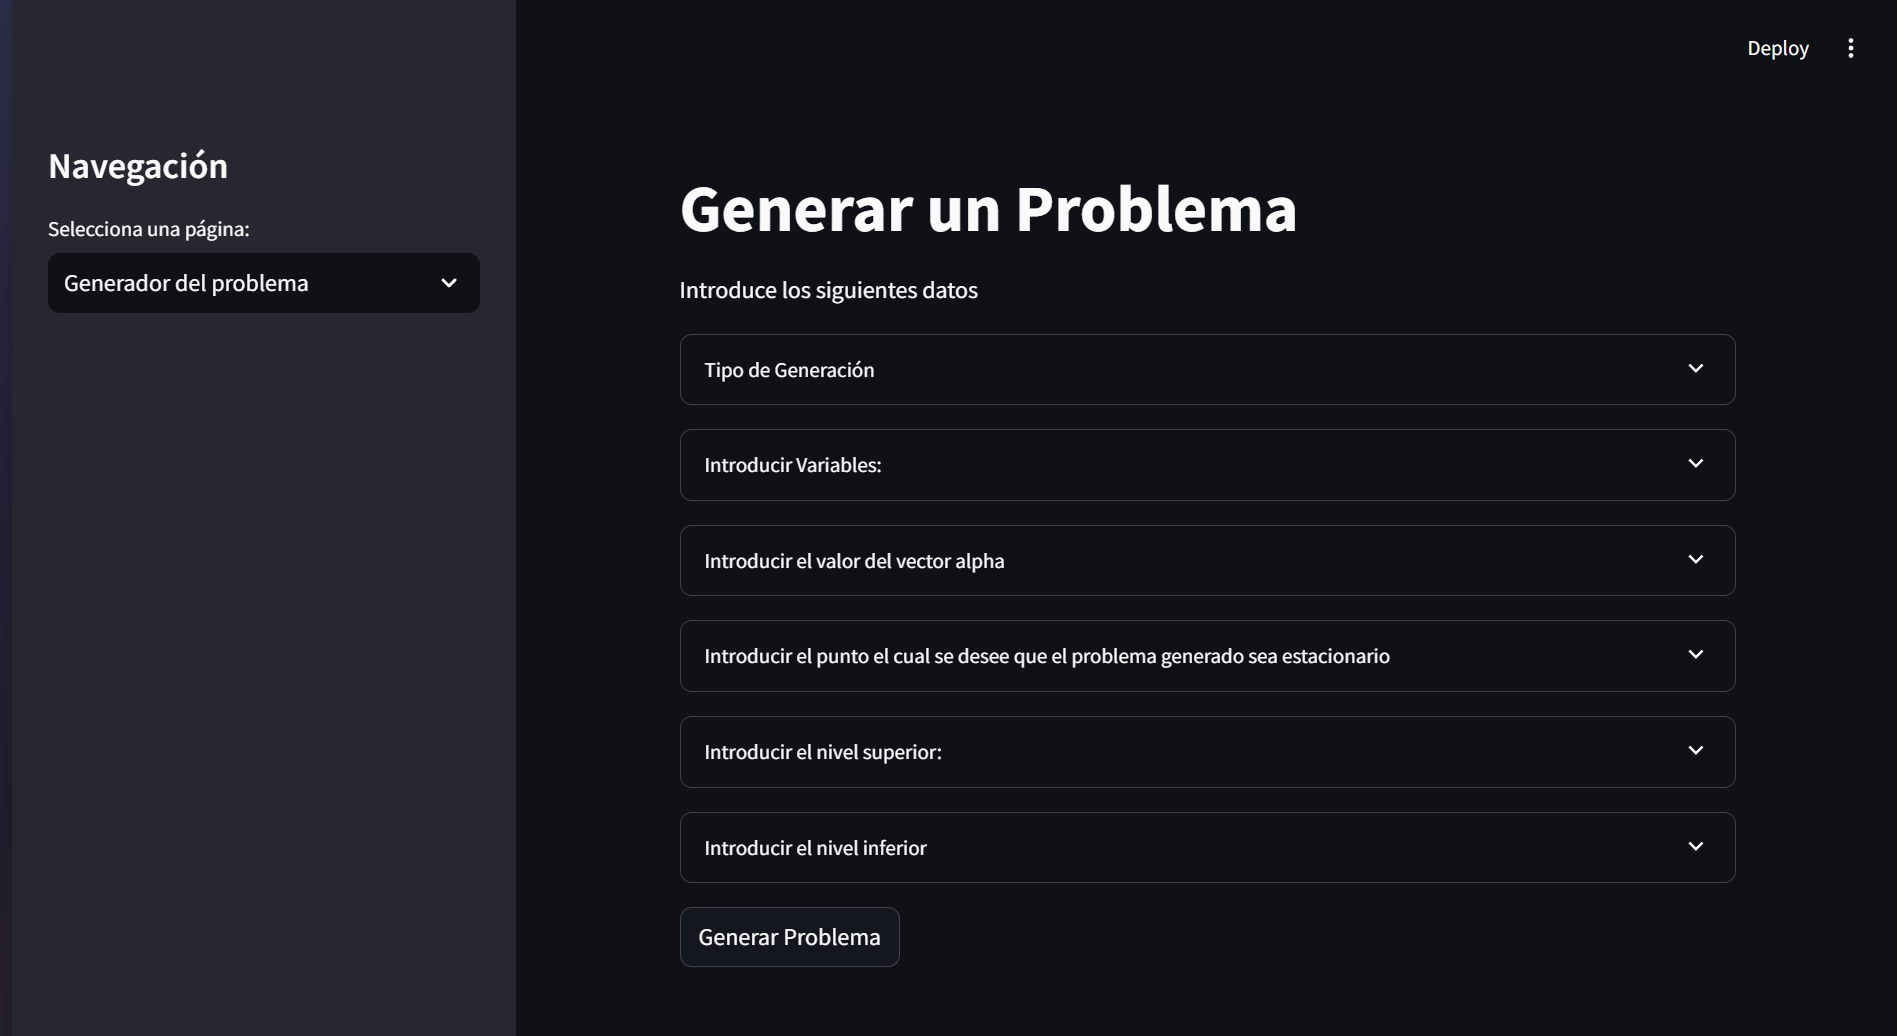
\includegraphics[width=\textwidth]{Graphics/front_streamlitpng.png}
    \caption{Pantalla principal de generación del problema}
    \label{fig:front_generator_page}
\end{figure}

\begin{figure}[H]
    \centering
    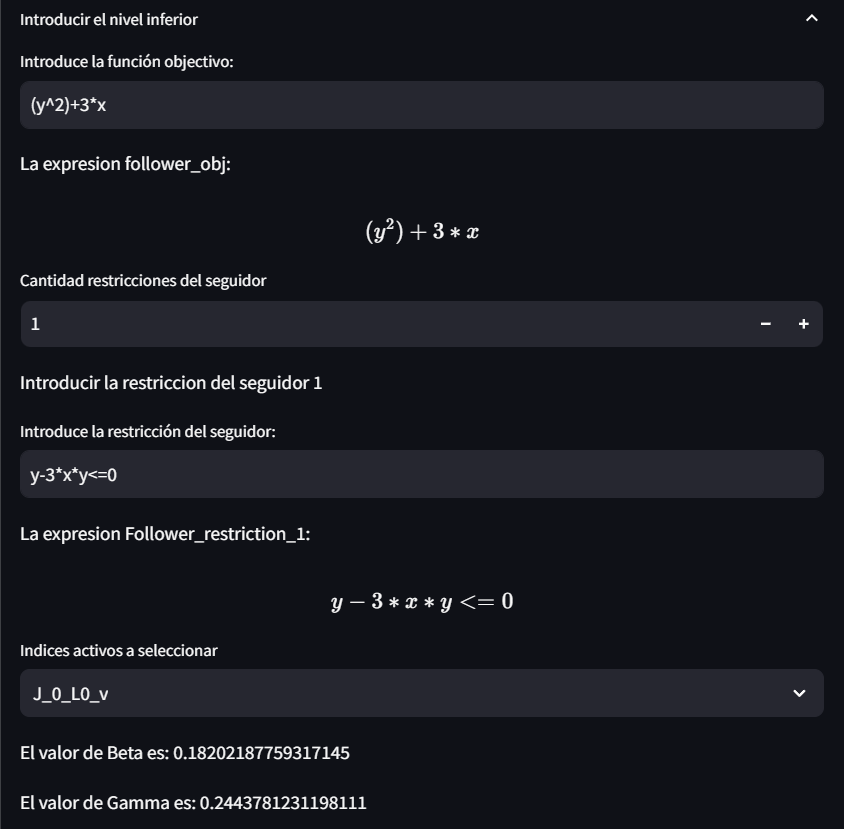
\includegraphics[width=\textwidth]{Graphics/Ejemplo_introducir_follower_rest.png}
    \caption{Ejemplo de generación de problema en punto Fuertemente Estacionario}
    \label{fig:example_strong_stationary_front_generator}
\end{figure}


\chapter{Experimentación}


En este capítulo se presenta la fase experimental basada en una selección de problemas de optimización binivel extraídos de la literatura especializada \cite{BolibTestProblems}. El estudio abarca tres categorías fundamentales de problemas: Lineales, Cuadráticos y No Convexos. La metodología experimental se desarrollará mediante la utilización de las bibliotecas de Julia para la identificación de mínimos locales, seguida de la perturbación de estos puntos mediante la introducción de valores aleatorios. A partir de estas modificaciones, se procederá a la generación de problemas estacionarios clasificados en 4 tipos específicos: $\alpha = 0$, C, M y fuerte

Los problemas modificados serán posteriormente evaluados utilizando algoritmos tradicionales implementados en Julia, con el objetivo de analizar su eficacia en relación al valor de la función objetivo del nivel superior. Este proceso permitirá determinar el impacto de las modificaciones realizadas y la robustez de los algoritmos frente a las variaciones introducidas.

Para garantizar un análisis exhaustivo y representativo, se han seleccionado un total de quince problemas de optimización binivel, distribuidos equitativamente entre las tres categorías mencionadas, asignando cinco problemas a cada una de ellas. Los problemas correspondientes a las categorías Lineales y Cuadráticos han sido extraídos de \cite{Floudas1999HandbookOT}, mientras que los problemas No Convexos provienen de \cite{BolibTestProblems}. Esta selección diversa permite una evaluación comprehensiva de las diferentes características y comportamientos de los problemas de optimización binivel bajo estudio.



\section{Modelación de la experimentación}
En esta sección se describe el proceso de experimentación, donde se toman las siguientes consideraciones. 
Todos los valores, han sido redondeados por exceso a dos cifras decimales. 
Los problemas escogidos para la experimentación son:

%Tabla con los problemas escogidos
\begin{table}[H]
\centering
\caption{Problemas Seleccionados}
\begin{tabular}{ | m{5cm} | m{5cm} | m{5cm} | }
  
  \hline
  \textbf{No Convexos} & \textbf{Lineales} & \textbf{Cuadráticos} \\
  \hline
  MitsosBarton2006Ex312 & ex9.1.1 & ex9.2.1 \\
  \hline
  MitsosBarton2006Ex313 & ex9.1.2 & ex9.2.2 \\
  \hline
  MitsosBarton2006Ex314 & ex9.1.8 & ex9.2.3\\
  \hline
  MitsosBarton2006Ex323 & ex9.1.9 & ex9.2.4\\
  \hline
  MorganPatrone2006a & ex9.1.10 & ex9.2.5 \\
  \hline
\end{tabular}
\end{table}

Inicialmente se computan óptimos de los problemas con los paquetes convencionales de Julia
cuya forma de resolver dependerá de la clase del problema. A continuación definiremos cada tipo de clase y como se obtienen los óptimos. 

% Definir problemas lineales

\begin{itemize}
    \item \textbf{Problemas Lineales y Cuadráticos :}\\
            Un problema binivel lineal es aquel en el cual los problemas del nivel superior e inferior son lineales, análogamente se define el problema cuadrático.
            % Escribir la definición matemática
            
            Con dicho problema se introducen los datos en la interfaz de \textbf{BilevelJuMP}, ver \cite{BilevelJump}, con el cual se utilizan 3 técnicas entre las ofrecidas por esta:
            \begin{itemize}
                \item \textbf{Big-M :} Con el optimizador High-Performance Solver for Linear Programming (HiGHS) y los valores $\text{primal big M} = 100, \quad \text{dual big M} = 100$.
                \item \textbf{SOS1 :} Con el optimizador Solving Constraint Integer Programs (SCIP).
                \item \textbf{ProductMode :} Con el optimizador Interior Point Optimizer (Ipopt).
            \end{itemize} 
            Cada uno de los resultados de evaluar el problema en cada forma anterior se guardan en un formato \textit{.xlsx}
            donde por cada optimizador se guardan los parámetros:
            \begin{itemize}
                \item Estatus del Primal, el cual define si es un punto factible o no.
                \item Estatus de la Finalización, si terminó porque encontró un óptimo o se estancó en un óptimo local.
                \item Valor de la función objetivo del nivel superior.
                \item El punto óptimo encontrado, en caso de ser hallado.
                \item El tiempo de ejecución.
            \end{itemize} 
            Posteriormente se analizan los resultados de dichos métodos, se selecciona el de mejor evaluación de la función objetivo.
    \item \textbf{Problemas No Convexos :}\\
            Al \textbf{BilevelJuMP} no contar con soporte para esta clase de problemas se utiliza \textbf{JuMP}, ver \cite{JuMPPaper}.
            Por ello se utiliza la reformulación KKT como la de \ref{eq:KKT_Optimista} y se procede a utilizar la interfaz brindada por este. Para el caso de las restricciones de 
            complementariedad se utiliza \textbf{Complementarity}, ver \cite{Complementarityjl}, con el optimizador Ipopt y análogo al caso anterior se extraen los mismos datos.
\end{itemize}


\subsubsection{Generación de los problemas}
Para la generación de los problemas, se toman los problemas seleccionados anteriormente con su punto óptimo calculado por las bibliotecas antes dichas, para ello mediante código de Julia se procede a generar los 4 tipos de problemas modificados: con \textit{$\alpha =0 $}, \textit{C-Estacionario}, \textit{M-Estacionario} y \textit{Fuertemente Estacionario}, mediante 
código de Julia para dichos experimentos. Cada experimento se realizará con semillas para poder replicarlos, cuya asignación se muestran en las tablas siguientes:



\begin{table}[h!]
\centering
\caption{Semillas utilizadas en problemas Lineales}
\begin{tabular}{ | m{5cm} | m{5cm} | m{5cm} | }
  
  \hline
  \textbf{No Convexos} & \textbf{Valor de la semilla para generar los problemas}  & \textbf{Valor de la semilla para hallar los óptimos de cada problema modificado} \\
  \hline
 ex9.1.1 & 20 & 6 \\
  \hline
 ex9.1.2 & 2 & 8\\
  \hline
   ex9.1.8 & 3& 9 \\
  \hline
  ex9.1.9 & 4 & 10\\
  \hline
 ex9.1.10 & 5 & 7 \\
  \hline
\end{tabular}
\end{table}


\begin{table}[h!]
    \centering
    \caption{Semillas utilizadas en problemas Cuadráticos}
    \begin{tabular}{ | m{5cm} | m{5cm} | m{5cm} | }
      
      \hline
      \textbf{No Convexos} & \textbf{Valor de la semilla para generar los problemas}  & \textbf{Valor de la semilla para hallar los óptimos de cada problema modificado} \\
      \hline
      ex9.2.1 & 11 &11 \\
      \hline
      ex9.2.2 & 12 &12 \\
      \hline
      ex9.2.3 & 13 &13\\
      \hline
      ex9.2.4 & 14 &14\\
      \hline
      ex9.2.5 & 15 &15\\
      \hline
    \end{tabular}
    \end{table}

    \begin{table}[h!]
        \centering
        \caption{Semillas utilizadas en problemas No Convexos}
        \begin{adjustbox}{max width=\textwidth}
        \begin{tabular}{ | m{5cm} | m{5cm} | m{5cm} | }
          
          \hline
          \textbf{No Convexos} & \textbf{Valor de la semilla para generar los problemas}  & \textbf{Valor de la semilla para hallar los óptimos de cada problema modificado} \\
          \hline
          MitsosBarton2006Ex312 & 6  & 1\\
          \hline
          MitsosBarton2006Ex313 & 7 & 2 \\
          \hline
          MitsosBarton2006Ex314 & 9 & 3\\
          \hline
          MitsosBarton2006Ex323 & 10 & 4\\
          \hline
          MorganPatrone2006a & 11 & 5 \\
          \hline
        \end{tabular}
     \end{adjustbox}
    \end{table}

    \section{Metodología de Generación y Experimentación}
    % Aclarar que son replicable
    % Aclarar que se divide en generar problemas, esos problemas guardarlos, después mandarlos a Julia a ver como rinden
    La experimentación consta de 3 partes fundamentales: generación del problema perturbado (para cumplir con cierta clase de estacionariedad en un punto dado), cómputo de óptimos del problema, análisis de los resultados.

    %
    Para la generación de los diferentes tipos de problemas perturbados utiliza semillas para la generación de los valores aleatorios para una replicación del mismo.
    La implementación sigue una sintaxis similar a la descrita en el capítulo anterior, dado que esta nueva implementación incorpora y extiende la anterior, pero permite 
    que con solo introducir un problema base se puedan generar los 4 tipos de problemas perturbados.
    
    El proceso de modificación de los puntos comienza con el problema original de entrada y el punto obtenido previamente. A cada componente de este punto se le añade un valor aleatorio en el intervalo $[1e-10, 5]$, obteniendo así el punto modificado $z^*_0$. Para los casos donde $\vec{\alpha}\neq \vec{0}$, se genera un vector aleatorio con componentes en el intervalo $[1e-10, 3]$. En cuanto a los conjuntos de índices activos de las $v_{j}s$, estos se distribuyen siguiendo una proporción específica: $1/2$ corresponde al tipo $J_1^v$ (\ref{J_0_lambda_0_level_inferior}), mientras que el $1/4$ restante se divide entre los tipos \ref{J_0_lambda_pos_level_inferior} y \ref{J_neg_lambda_0_level_inferior}.
    
    La selección de los multiplicadores $\lambda_j$ $\beta_j$ y $\gamma_j$ se realiza mediante la generación de valores aleatorios en el intervalo $[1e-2, 10]$ cuando estos no deben ser $0$. En los casos donde existen múltiples combinaciones posibles de multiplicadores con respecto a su igualdad a $0$, se utiliza una distribución uniforme discreta para la selección aleatoria.
    
    Cada problema generado se almacena en un archivo \textit{.xlsx} siguiendo la nomenclatura: \textit{(nombre del problema)\_(Tipo de punto estacionario)(generator)\_alpha\_((non\_zero) si $\alpha \neq 0$ y (zero) si $\alpha = 0$).xlsx}. Este archivo contiene la información completa del problema, incluyendo las expresiones de las funciones objetivo de ambos niveles con sus evaluaciones en el punto, las restricciones de ambos niveles con sus respectivos multiplicadores y tipos de índices activos, el punto $z^*_0$, los vectores $\vec{bf}$ y $\vec{BF}$, y el multiplicador $\vec{\alpha}$.
    
    La compilación y procesamiento posterior se realiza mediante un script de Python que utiliza las dependencias \textit{pandas} y \textit{sympy}. Este script procesa la información contenida en los archivos \textit{.xlsx} y genera scripts \textit{.jl} con el módulo de experimentación para la obtención de valores óptimos. La ejecución de estos scripts se gestiona mediante \textit{subprocess}, y los resultados se recopilan para identificar los casos más relevantes y generar tanto el código latex de cada problema modificado como las tablas de resultados correspondientes.
    
    %Análisis Comparativo de Algoritmos
    
    %Presentación de Resultados
    Los resultados seleccionados se presentan en tablas estructuradas que incluyen información fundamental para cada problema, hay una por cada tipo de problema y tipo de punto lo que hace una total de 12. Estas tablas contienen el nombre del problema original que fue modificado para alcanzar la estacionariedad de la clase deseada, el punto al cual se forzó ser estacionario de la clase requerida (asegurando que no pertenezca a un subconjunto de esta), la evaluación de la función objetivo en el punto estacionario, el punto óptimo identificado por los algoritmos de Julia, la evaluación de la función objetivo en este óptimo, el método seleccionado para su obtención y el tiempo requerido para su ejecución. Además al final de cada tipo de problema existe una tabla la cual por cada tipo de punto se pone un problema característico el cual obtuvo mejor evaluación de la función objetivo con respecto al del mejor óptimo.



\subsection{Problemas Lineales} 
  
\subsubsection{Tablas}
\begin{resultstablee}{Resultados de los problemas Lineal del tipo Alpha-Zero}
    
    \resultroww{ex9.1.1}{( 6.05, 6.85, 3.10,)}{18.59}{( 6.13, 6.85, -173.65,)}{-1820.0}{Highs-BigM (100,100)}{FEASIBLE-POINT}{OPTIMAL}{0.00046779663909999995} 
\resultroww{ex9.1.1}{( 6.05, 6.85, 3.10,)}{18.59}{( 6.13, 6.85, -1.19e+19,)}{-1.2384285244918673e+20}{ProductMode}{NEARLY-FEASIBLE-POINT}{ALMOST-LOCALLY-SOLVED}{0.018216050283636365} 
 \hline  
 \resultroww{ex9.1.10}{( 51.55, 18.10, 102.20, 0.20,)}{-0.48}{( 1.65, 34.73, 102.20, 100.00,)}{-240.0}{Highs-BigM (100,100)}{FEASIBLE-POINT}{OPTIMAL}{0.0005916887039552061} 
\resultroww{ex9.1.10}{( 51.55, 18.10, 102.20, 0.20,)}{-0.48}{( -1.01e+20, 3.37e+19, 676781.00, 2.02e+20,)}{-4.8528604996887255e+20}{ProductMode}{INFEASIBLE-POINT}{NORM-LIMIT}{0.09548243956603773} 
 \hline  
 \resultroww{ex9.1.2}{( 7.00, 8.95,)}{0.0}{( 7.00, 8.95,)}{0}{Highs-BigM (100,100)}{FEASIBLE-POINT}{OPTIMAL}{0.0005095908938271605} 
\resultroww{ex9.1.2}{( 7.00, 8.95,)}{0.0}{( 7.00, 8.95,)}{0}{SOS1}{FEASIBLE-POINT}{OPTIMAL}{0.0036491232397660818} 
\resultroww{ex9.1.2}{( 7.00, 8.95,)}{0.0}{( 7.00, 8.95,)}{0}{ProductMode}{FEASIBLE-POINT}{LOCALLY-SOLVED}{0.012145625483009709} 
 \hline  
 \resultroww{ex9.1.8}{( 4.50, 1.60, 6.10, 1.55,)}{0.0}{( -200.00, 0.00, -203.20, 201.25,)}{0}{Highs-BigM (100,100)}{FEASIBLE-POINT}{OPTIMAL}{0.0006034477299367704} 
\resultroww{ex9.1.8}{( 4.50, 1.60, 6.10, 1.55,)}{0.0}{( 5.14, 1.30, 5.82, 0.00,)}{0}{SOS1}{FEASIBLE-POINT}{OPTIMAL}{0.003330911396264176} 
\resultroww{ex9.1.8}{( 4.50, 1.60, 6.10, 1.55,)}{0.0}{( -3837804609426.00, 3837804592535.52, 7675609168177.35, 15351218387033.80,)}{0}{ProductMode}{INFEASIBLE-POINT}{OTHER-ERROR}{0.0392210034453125} 
 \hline  
 \resultroww{ex9.1.9}{( 4.78, 6.17,)}{3.98}{( 8.61, -1.48,)}{-2.9}{Highs-BigM (100,100)}{FEASIBLE-POINT}{OPTIMAL}{0.0004643262269} 
\resultroww{ex9.1.9}{( 4.78, 6.17,)}{3.98}{( 8.61, -1.48,)}{-2.9}{SOS1}{FEASIBLE-POINT}{OPTIMAL}{0.005123980320000001} 
\resultroww{ex9.1.9}{( 4.78, 6.17,)}{3.98}{( 4.79, 6.17,)}{3.98}{ProductMode}{FEASIBLE-POINT}{LOCALLY-SOLVED}{0.009638699485549133} 
 \hline  

 \end{resultstablee}   


 \begin{resultstablee}{Resultados de los problemas Lineal del tipo C-Estacionario}
    
    \resultroww{ex9.1.1}{( 6.05, 6.85, 3.10,)}{74.95}{( 0.00, 0.00, 0.00,)}{0.0}{Highs-BigM (100,100)}{NO-SOLUTION}{INFEASIBLE}{0.0004682440455} 
\resultroww{ex9.1.1}{( 6.05, 6.85, 3.10,)}{74.95}{( 6.25, 10.36, 6.60,)}{-27.94}{ProductMode}{INFEASIBLE-POINT}{LOCALLY-INFEASIBLE}{0.01053818123628692} 
 \hline  
 \resultroww{ex9.1.10}{( 51.55, 18.10, 102.20, 0.20,)}{0.0}{( 50.81, 17.80, 126.86, 163.97,)}{0}{Highs-BigM (100,100)}{FEASIBLE-POINT}{OPTIMAL}{0.0006909111494300806} 
\resultroww{ex9.1.10}{( 51.55, 18.10, 102.20, 0.20,)}{0.0}{( 53.73, 19.59, 0.00, -664.87,)}{0}{SOS1}{FEASIBLE-POINT}{OPTIMAL}{0.003464193543372658} 
\resultroww{ex9.1.10}{( 51.55, 18.10, 102.20, 0.20,)}{0.0}{( 50.81, 17.80, 126.75, 163.24,)}{0}{ProductMode}{FEASIBLE-POINT}{LOCALLY-SOLVED}{0.0068813606955922865} 
 \hline  
 \resultroww{ex9.1.2}{( 7.00, 8.95,)}{-533.33}{( 7.00, 8.95,)}{-533.62}{Highs-BigM (100,100)}{FEASIBLE-POINT}{OPTIMAL}{0.00036514324190000004} 
\resultroww{ex9.1.2}{( 7.00, 8.95,)}{-533.33}{( 7.00, 8.95,)}{-533.62}{SOS1}{FEASIBLE-POINT}{OPTIMAL}{0.0028385706895963617} 
\resultroww{ex9.1.2}{( 7.00, 8.95,)}{-533.33}{( 7.00, 8.95,)}{-533.62}{ProductMode}{FEASIBLE-POINT}{LOCALLY-SOLVED}{0.011949152739234449} 
 \hline  
 \resultroww{ex9.1.8}{( 4.50, 1.60, 6.10, 1.55,)}{0.0}{( 0.00, 0.00, 0.00, 0.00,)}{0}{Highs-BigM (100,100)}{NO-SOLUTION}{INFEASIBLE}{0.0004503267894} 
\resultroww{ex9.1.8}{( 4.50, 1.60, 6.10, 1.55,)}{0.0}{( 4.79, 1.52, -4.91, 0.00,)}{0}{SOS1}{FEASIBLE-POINT}{OPTIMAL}{0.003091181772136223} 
\resultroww{ex9.1.8}{( 4.50, 1.60, 6.10, 1.55,)}{0.0}{( 157622.80, -157616.49, -204903418.75, -19264423.52,)}{0}{ProductMode}{FEASIBLE-POINT}{LOCALLY-SOLVED}{0.006741560248313091} 
 \hline  
 \resultroww{ex9.1.9}{( 4.78, 6.17,)}{-359.91}{( 0.00, 0.00,)}{0.0}{Highs-BigM (100,100)}{NO-SOLUTION}{INFEASIBLE}{0.0005221321025021026} 
\resultroww{ex9.1.9}{( 4.78, 6.17,)}{-359.91}{( 4.78, 6.68,)}{-385.79}{ProductMode}{INFEASIBLE-POINT}{LOCALLY-INFEASIBLE}{0.005467831646608316} 
 \hline  
 \end{resultstablee} 


 
 \begin{resultstablee}{Resultados de los problemas Lineal del tipo M-Estacionario}
 
 \resultroww{ex9.1.1}{( 6.05, 6.85, 3.10,)}{-350.25}{( 0.00, 0.00, 0.00,)}{0.0}{Highs-BigM (100,100)}{NO-SOLUTION}{INFEASIBLE}{0.0006334388676526839} 
\resultroww{ex9.1.1}{( 6.05, 6.85, 3.10,)}{-350.25}{( 6.10, 2.56, 0.19,)}{-353.19}{ProductMode}{INFEASIBLE-POINT}{LOCALLY-INFEASIBLE}{0.009341708173831776} 
\hline  
\resultroww{ex9.1.10}{( 51.55, 18.10, 102.20, 0.20,)}{256.63}{( -561.59, -215.62, -247.16, -207.74,)}{255.12}{Highs-BigM (100,100)}{FEASIBLE-POINT}{OPTIMAL}{0.0007100866538461538} 
\resultroww{ex9.1.10}{( 51.55, 18.10, 102.20, 0.20,)}{256.63}{( -405840425249201.62, -154685870165387.44, -231326563895116.47, -137694383270963.31,)}{-440622026211.5}{ProductMode}{INFEASIBLE-POINT}{ITERATION-LIMIT}{0.659487631} 
\hline  
\resultroww{ex9.1.2}{( 7.00, 8.95,)}{-42.7}{( 0.00, 0.00,)}{0.0}{Highs-BigM (100,100)}{NO-SOLUTION}{INFEASIBLE}{0.0004965854824447335} 
\resultroww{ex9.1.2}{( 7.00, 8.95,)}{-42.7}{( 0.31, 0.13,)}{-1.87}{ProductMode}{INFEASIBLE-POINT}{LOCALLY-INFEASIBLE}{0.00501175204321608} 
\hline  
\resultroww{ex9.1.8}{( 4.50, 1.60, 6.10, 1.55,)}{-17.69}{( 0.00, 0.00, 0.00, 0.00,)}{0.0}{Highs-BigM (100,100)}{NO-SOLUTION}{INFEASIBLE}{0.00045952245730000003} 
\resultroww{ex9.1.8}{( 4.50, 1.60, 6.10, 1.55,)}{-17.69}{( -0.14, 0.43, -0.13, 0.12,)}{-0.83}{ProductMode}{INFEASIBLE-POINT}{LOCALLY-INFEASIBLE}{0.004769426563097514} 
\hline  
\resultroww{ex9.1.9}{( 4.78, 6.17,)}{0.0}{( 4.78, 6.16,)}{0}{Highs-BigM (100,100)}{FEASIBLE-POINT}{OPTIMAL}{0.0004206910923} 
\resultroww{ex9.1.9}{( 4.78, 6.17,)}{0.0}{( 4.78, 6.16,)}{0}{SOS1}{FEASIBLE-POINT}{OPTIMAL}{0.00354871923541963} 
\resultroww{ex9.1.9}{( 4.78, 6.17,)}{0.0}{( -99475.59, -82209.03,)}{0}{ProductMode}{FEASIBLE-POINT}{LOCALLY-SOLVED}{0.007394484687407407} 
\hline  

 
 
\end{resultstablee}

\begin{resultstablee}{Resultados de los problemas Lineal del tipo Fuertemente-Estacionario}
    
    \resultroww{ex9.1.1}{( 6.05, 6.85, 3.10,)}{-195.55}{( 6.14, 6.84, 3.11,)}{-195.39}{Highs-BigM (100,100)}{FEASIBLE-POINT}{OPTIMAL}{0.0017798902932761088} 
\resultroww{ex9.1.1}{( 6.05, 6.85, 3.10,)}{-195.55}{( 6.14, 6.84, 3.11,)}{-195.39}{SOS1}{FEASIBLE-POINT}{OPTIMAL}{0.005630886166854566} 
\resultroww{ex9.1.1}{( 6.05, 6.85, 3.10,)}{-195.55}{( 6.14, 6.84, 3.11,)}{-195.39}{ProductMode}{FEASIBLE-POINT}{LOCALLY-SOLVED}{0.00896522621005386} 
 \hline  
 \resultroww{ex9.1.10}{( 51.55, 18.10, 102.20, 0.20,)}{-17921.11}{( 0.00, 0.00, 0.00, 0.00,)}{0.0}{Highs-BigM (100,100)}{NO-SOLUTION}{INFEASIBLE}{0.0005715590879475077} 
\resultroww{ex9.1.10}{( 51.55, 18.10, 102.20, 0.20,)}{-17921.11}{( -151.11, 3.00, 39.70, -20.88,)}{-5686.3}{ProductMode}{INFEASIBLE-POINT}{LOCALLY-INFEASIBLE}{0.010776944681034482} 
 \hline  
 \resultroww{ex9.1.2}{( 7.00, 8.95,)}{-957.15}{( 0.00, 0.00,)}{0.0}{Highs-BigM (100,100)}{NO-SOLUTION}{INFEASIBLE}{0.0006340764801227152} 
\resultroww{ex9.1.2}{( 7.00, 8.95,)}{-957.15}{( 7.00, 2.20,)}{-325.17}{ProductMode}{INFEASIBLE-POINT}{LOCALLY-INFEASIBLE}{0.007307757475146198} 
 \hline  
 \resultroww{ex9.1.8}{( 4.50, 1.60, 6.10, 1.55,)}{-222.34}{( 0.00, 0.00, 0.00, 0.00,)}{0.0}{Highs-BigM (100,100)}{NO-SOLUTION}{INFEASIBLE}{0.0006772643256480219} 
\resultroww{ex9.1.8}{( 4.50, 1.60, 6.10, 1.55,)}{-222.34}{( -1180748808400.02, 46459818920.77, -1663916387913.37, 1630567769460.85,)}{-82526799750.46}{ProductMode}{INFEASIBLE-POINT}{LOCALLY-INFEASIBLE}{0.05180543995876288} 
 \hline  
 \resultroww{ex9.1.9}{( 4.78, 6.17,)}{-542.78}{( 4.78, 6.17,)}{-542.6}{Highs-BigM (100,100)}{FEASIBLE-POINT}{OPTIMAL}{0.00045500844910000005} 
\resultroww{ex9.1.9}{( 4.78, 6.17,)}{-542.78}{( 4.78, 6.17,)}{-542.6}{SOS1}{FEASIBLE-POINT}{OPTIMAL}{0.004884637435972629} 
\resultroww{ex9.1.9}{( 4.78, 6.17,)}{-542.78}{( 4.78, 6.17,)}{-542.6}{ProductMode}{FEASIBLE-POINT}{LOCALLY-SOLVED}{0.00781831336973479} 
 \hline  
 
    
    
 \end{resultstablee} 

 \begin{resultstable}{Problemas Lineal Seleccionados}
    \resultrow{$\alpha=0$}{ex9.1.1}{( 6.05, 6.85, 3.1,)}{18.59}{( -173.65,)}{-1820.0}{Highs-BigM (100,100)}
    \resultrow{C-Estacionario}{ex9.1.8}{( 4.50, 1.60, 6.10, 1.55,)}{0.0}{( 157622.80, -157616.49, -204903418.75, -19264423.52,)}{0}{ProductMode}
    \resultrow{M-Estacionario}{ex9.1.9}{( 4.78, 6.17,)}{0.0}{( -99475.59, -82209.03,)}{0}{ProductMode}
    \resultrow{Fuertemente-Estacionario}{ex9.1.1}{( 6.05, 6.85, 3.10,)}{-195.55}{( 6.14, 6.84, 3.11,)}{-195.39}{Highs-BigM (100,100)}
    \end{resultstable}

%region Resultados Lineales

%region Alpha-zero

\subsubsection{$\alpha =0$}

%Analisis
En los problemas de Alpha Zero, se mostró cierta complejidad para SOS1, el cual en algunos casos no pudo determinar puntos, mientras que Big-M logró completar los objetivos. 
Los puntos hallados en los problemas eran mayoritariamente distantes en sus componentes con respecto al punto estacionario original,  indicando que el posible valor óptimo no está en una vecindad del punto inicial, siendo la diferencia de componente a componente, tan grande como $1e+20$.
En términos generales de rendimiento, Big-M tuvo un excelente desempeño, seguido de SOS1 y por último de ProductMode. 
En este caso el problema que mayor mejora tuvo fue el ex9.1.1
%endregion

%region C-Estacionario
\subsubsection{C-Estacionario}
    
 En los problemas de C-Estacionario donde la evaluación del punto estacionario inicial es 0, no mejoró el valor de la función objetivo evaluada en el óptimo. El método Big-M tuvo problemas para hallar el óptimo, probablemente debido a los valores extremos de este.

 
 
    
%endregion   
 

\subsubsection{M-Estacionario}

 En los problemas de M-Estacionario, los algoritmos tuvieron grandes dificultades para encontrar el óptimo. 
 Los problemas ex9.1.10 y ex9.1.9 son los únicos en los que Julia halló puntos óptimos, en el primero halló un punto óptimo cuya evaluación es cercana a la del punto estacionario inicial aunque sin estar en una vecindad de este, el segundo halló mediante Big-M y SOS1 puntos óptimos que están en la vecindad del punto estacionario inicial y  ProductMode localizó un punto óptimo cuya evaluación es igual a la evaluación del punto estacionario inicial aunque este no se encuentra en una vecindad. ProductMode tuvo complicaciones para hallar los óptimos en este tipo de problemas.
 
  
\subsubsection{Fuertemente Estacionario}
    
 En los problemas de tipo Fuertemente Estacionario, los métodos de Julia presentaron complicaciones  en  ex9.1.1 y ex9.1.9 donde en ambos casos Big-M, SOS1 y ProductMode hallaron puntos óptimos en la vecindad del punto estacionario inicial.


%region Best Lineales
\subsubsection{Problemas relevantes de cada categoría de punto:}
 


    
%endregion
En los problemas analizados se evidencia que mientras más fuertes sean las condiciones de los puntos es más probable de hallar óptimos en la vecindad del punto original, 
así como también es probable que los algoritmos no logren encontrar un valor óptimo y terminen con puntos insatisfactibles.
El método SOS1 tuvo dificultades para obtener alguna solución, mientras que Big-M tuvo mayormente problemas asociados a sus valores extremos, teniendo ProductMode un comportamiento similar a este aunque con mayor tiempo de cómputo.
Además no existe caso en el que el valor objetivo halla sido peor que el valor inicial estacionario.
   

%endregion
% C-Estacionario

\subsection{Problemas Cuadráticos}


\begin{resultstablee}{Resultados de los problemas Cuadrático del tipo Alpha-Zero}
    	    
    \resultroww{ex9.2.1}{( 1.85, 4.65,)}{-106.29}{( 2.19, 5.31,)}{-108.96}{SOS1}{FEASIBLE-POINT}{OPTIMAL}{0.01085754318478261} 
\resultroww{ex9.2.1}{( 1.85, 4.65,)}{-106.29}{( 2.19, 5.31,)}{-108.96}{ProductMode}{FEASIBLE-POINT}{LOCALLY-SOLVED}{0.007574700737878789} 
 \hline  
 \resultroww{ex9.2.2}{( 14.45, 14.40,)}{-415.5}{( 14.45, 14.40,)}{-415.5}{SOS1}{FEASIBLE-POINT}{OPTIMAL}{0.002536806859319452} 
\resultroww{ex9.2.2}{( 14.45, 14.40,)}{-415.5}{( 14.45, 14.40,)}{-415.5}{ProductMode}{FEASIBLE-POINT}{LOCALLY-SOLVED}{0.00493924387734916} 
 \hline  
 \resultroww{ex9.2.3}{( 1.55, 2.70, -5.10, -8.65,)}{8.98}{( -3.85, 2.70, -5.10, -11.35,)}{30.31}{Highs-BigM (100,100)}{FEASIBLE-POINT}{OPTIMAL}{0.0014682835419126327} 
\resultroww{ex9.2.3}{( 1.55, 2.70, -5.10, -8.65,)}{8.98}{( -3.85, 2.70, -5.10, -11.35,)}{30.31}{SOS1}{FEASIBLE-POINT}{OPTIMAL}{0.006388017097186701} 
\resultroww{ex9.2.3}{( 1.55, 2.70, -5.10, -8.65,)}{8.98}{( -3.85, 2.70, -5.10, -11.35,)}{30.31}{ProductMode}{NEARLY-FEASIBLE-POINT}{ALMOST-LOCALLY-SOLVED}{0.01848814341697417} 
 \hline  
 \resultroww{ex9.2.4}{( 4.25, 4.85, 4.70,)}{-91.56}{( 0.15, 4.85, -4.70,)}{43.8}{SOS1}{FEASIBLE-POINT}{OPTIMAL}{0.0032146947907276237} 
\resultroww{ex9.2.4}{( 4.25, 4.85, 4.70,)}{-91.56}{( 0.15, 4.85, -4.70,)}{43.8}{ProductMode}{FEASIBLE-POINT}{LOCALLY-SOLVED}{0.004554985538742023} 
 \hline  
 \resultroww{ex9.2.5}{( 4.75, 4.05,)}{3.4}{( 4.75, 4.05,)}{3.4}{SOS1}{FEASIBLE-POINT}{OPTIMAL}{0.017031251261904762} 
\resultroww{ex9.2.5}{( 4.75, 4.05,)}{3.4}{( 4.75, 4.05,)}{3.4}{ProductMode}{FEASIBLE-POINT}{LOCALLY-SOLVED}{0.00521551028914405} 
 \hline      
 \end{resultstablee} 


 \begin{resultstablee}{Resultados de los problemas Cuadrático del tipo C-Estacionario}
    
    \resultroww{ex9.2.1}{( 1.85, 4.65,)}{-17.97}{( 1.85, 2.39,)}{16.72}{SOS1}{FEASIBLE-POINT}{OPTIMAL}{0.030418006612121212} 
\resultroww{ex9.2.1}{( 1.85, 4.65,)}{-17.97}{( 1.85, 2.39,)}{16.72}{ProductMode}{FEASIBLE-POINT}{LOCALLY-SOLVED}{0.04917132575490196} 
 \hline  
 \resultroww{ex9.2.2}{( 14.45, 14.40,)}{-1327.11}{( 14.48, 14.40,)}{-1327.01}{SOS1}{FEASIBLE-POINT}{OPTIMAL}{0.003636090177713037} 
\resultroww{ex9.2.2}{( 14.45, 14.40,)}{-1327.11}{( 14.48, 14.40,)}{-1327.01}{ProductMode}{FEASIBLE-POINT}{LOCALLY-SOLVED}{0.0051832394190871375} 
 \hline  
 \resultroww{ex9.2.3}{( 1.55, 2.70, -5.10, -8.65,)}{363.83}{( -0.18, 49.63, 5.89, 19.45,)}{-548.42}{Highs-BigM (100,100)}{FEASIBLE-POINT}{OPTIMAL}{0.0045629535242451965} 
\resultroww{ex9.2.3}{( 1.55, 2.70, -5.10, -8.65,)}{363.83}{( 32.97, -5.86, 15.95, 13.31,)}{-1201.53}{SOS1}{FEASIBLE-POINT}{OPTIMAL}{0.0051704202712215324} 
\resultroww{ex9.2.3}{( 1.55, 2.70, -5.10, -8.65,)}{363.83}{( -0.18, 49.63, 5.89, 19.45,)}{-548.42}{ProductMode}{FEASIBLE-POINT}{LOCALLY-SOLVED}{0.004764864257633587} 
 \hline  
 \resultroww{ex9.2.4}{( 4.25, 4.85, 4.70,)}{-33.88}{( -4.22, -0.13, -4.09,)}{11.48}{SOS1}{FEASIBLE-POINT}{OPTIMAL}{0.0038767353470178156} 
\resultroww{ex9.2.4}{( 4.25, 4.85, 4.70,)}{-33.88}{( -4.22, -0.13, -4.09,)}{11.48}{ProductMode}{FEASIBLE-POINT}{LOCALLY-SOLVED}{0.003738380746067416} 
 \hline  
 \resultroww{ex9.2.5}{( 4.75, 4.05,)}{-42.78}{( 4.43, 4.19,)}{-42.9}{SOS1}{FEASIBLE-POINT}{OPTIMAL}{0.011993493127098322} 
\resultroww{ex9.2.5}{( 4.75, 4.05,)}{-42.78}{( 4.43, 4.19,)}{-42.9}{ProductMode}{FEASIBLE-POINT}{LOCALLY-SOLVED}{0.003723685645786726} 
 \hline  
 \end{resultstablee} 

 \begin{resultstablee}{Resultados de los problemas Cuadrático del tipo M-Estacionario}
    
    \resultroww{ex9.2.1}{( 1.85, 4.65,)}{-41.57}{( 1.85, 4.61,)}{-41.63}{SOS1}{FEASIBLE-POINT}{OPTIMAL}{0.003688455623059867} 
\resultroww{ex9.2.1}{( 1.85, 4.65,)}{-41.57}{( 1.85, 4.61,)}{-41.63}{ProductMode}{FEASIBLE-POINT}{LOCALLY-SOLVED}{0.0146413623625731} 
 \hline  
 \resultroww{ex9.2.2}{( 14.45, 14.40,)}{-619.42}{( 11.02, 9.49,)}{-488.71}{SOS1}{FEASIBLE-POINT}{OPTIMAL}{0.019986648072} 
\resultroww{ex9.2.2}{( 14.45, 14.40,)}{-619.42}{( 11.02, 9.49,)}{-488.71}{ProductMode}{FEASIBLE-POINT}{LOCALLY-SOLVED}{0.0027599958350857778} 
 \hline  
 \resultroww{ex9.2.3}{( 1.55, 2.70, -5.10, -8.65,)}{405.85}{( 1.48, 2.65, -5.08, -8.66,)}{404.57}{Highs-BigM (100,100)}{FEASIBLE-POINT}{OPTIMAL}{0.001168006057492931} 
\resultroww{ex9.2.3}{( 1.55, 2.70, -5.10, -8.65,)}{405.85}{( 1.48, 2.65, -5.08, -8.66,)}{404.57}{SOS1}{FEASIBLE-POINT}{OPTIMAL}{0.0031234532765957446} 
\resultroww{ex9.2.3}{( 1.55, 2.70, -5.10, -8.65,)}{405.85}{( 1.48, 2.65, -5.08, -8.66,)}{404.57}{ProductMode}{FEASIBLE-POINT}{LOCALLY-SOLVED}{0.00878768395606327} 
 \hline  
 \resultroww{ex9.2.4}{( 4.25, 4.85, 4.70,)}{-53.06}{( -303.76, -14.82, -288.94,)}{43860.69}{SOS1}{FEASIBLE-POINT}{OPTIMAL}{0.006881493973829201} 
\resultroww{ex9.2.4}{( 4.25, 4.85, 4.70,)}{-53.06}{( -303.76, -14.82, -288.94,)}{43860.69}{ProductMode}{FEASIBLE-POINT}{LOCALLY-SOLVED}{0.004288314234536082} 
 \hline  
 \resultroww{ex9.2.5}{( 4.75, 4.05,)}{-123.02}{( 4.73, 4.06,)}{-123.3}{SOS1}{FEASIBLE-POINT}{OPTIMAL}{0.028344932163841808} 
\resultroww{ex9.2.5}{( 4.75, 4.05,)}{-123.02}{( 4.73, 4.06,)}{-123.3}{ProductMode}{FEASIBLE-POINT}{LOCALLY-SOLVED}{0.0050364884899193555} 
 \hline  
 \end{resultstablee} 

 \begin{resultstablee}{Resultados de los problemas Cuadrático del tipo Fuertemente-Estacionario}
    
    \resultroww{ex9.2.1}{( 1.85, 4.65,)}{-379.69}{( 1.85, 4.65,)}{-379.65}{SOS1}{FEASIBLE-POINT}{OPTIMAL}{0.008176077955810147} 
\resultroww{ex9.2.1}{( 1.85, 4.65,)}{-379.69}{( 1.85, 4.65,)}{-379.65}{ProductMode}{FEASIBLE-POINT}{LOCALLY-SOLVED}{0.005971634445639188} 
 \hline  
 \resultroww{ex9.2.2}{( 14.45, 14.40,)}{-2976.34}{( 14.45, 14.40,)}{-2976.34}{ProductMode}{INFEASIBLE-POINT}{LOCALLY-INFEASIBLE}{0.006671206622162884} 
 \hline  
 \resultroww{ex9.2.3}{( 1.55, 2.70, -5.10, -8.65,)}{293.57}{( -6.90, -7.39, 0.87, -12.87,)}{111.17}{Highs-BigM (100,100)}{FEASIBLE-POINT}{OPTIMAL}{0.0013926462687237028} 
\resultroww{ex9.2.3}{( 1.55, 2.70, -5.10, -8.65,)}{293.57}{( -6.90, -7.39, 0.87, -12.87,)}{111.17}{SOS1}{FEASIBLE-POINT}{OPTIMAL}{0.003255103333767927} 
\resultroww{ex9.2.3}{( 1.55, 2.70, -5.10, -8.65,)}{293.57}{( -6.90, -7.39, 0.87, -12.87,)}{111.17}{ProductMode}{FEASIBLE-POINT}{LOCALLY-SOLVED}{0.020168756826612906} 
 \hline  
 \resultroww{ex9.2.4}{( 4.25, 4.85, 4.70,)}{-23.39}{( -46.77, 0.00, -76.20,)}{3537.11}{ProductMode}{INFEASIBLE-POINT}{LOCALLY-INFEASIBLE}{0.006134994812039312} 
 \hline  
 \resultroww{ex9.2.5}{( 4.75, 4.05,)}{-197.17}{( -0.56, 4.83,)}{-236.14}{SOS1}{FEASIBLE-POINT}{OPTIMAL}{0.007121795407988588} 
\resultroww{ex9.2.5}{( 4.75, 4.05,)}{-197.17}{( -0.56, 4.83,)}{-236.14}{ProductMode}{FEASIBLE-POINT}{LOCALLY-SOLVED}{0.007361066086892489} 
 \hline  

 \end{resultstablee} 


    
\begin{resultstable}{Problemas Cuadrático Seleccionados}
    \resultrow{$\alpha=0$}{ex9.2.1}{( 1.85, 4.65,)}{-106.29}{( 2.19, 5.31,)}{-108.96}{ProductMode}
    \resultrow{C-Estacionario}{ex9.2.3}{( 1.55, 2.70, -5.10, -8.65,)}{363.83}{( 32.97, -5.86, 15.95, 13.31,)}{-1201.53}{SOS1}
    \resultrow{M-Estacionario}{ex9.2.3}{( 1.55, 2.70, -5.10, -8.65,)}{405.85}{( 1.48, 2.65, -5.08, -8.66,)}{404.57}{Highs-BigM (100,100)}
    \resultrow{Fuertemente-Estacionario}{ex9.2.3}{( 1.55, 2.70, -5.10, -8.65,)}{293.57}{( -6.90, -7.39, 0.87, -12.87,)}{111.17}{Highs-BigM (100,100)} 
    \end{resultstable}
    
%region Resultados Cuadraticos
\subsubsection{$\alpha =0$}
    	
         En los problemas ex9.2.3 y ex9.2.4, los métodos encontraron puntos cuyo valor de la función objetivo es considerablemente peor que el del punto estacionario inicial. 
         En estos casos, los puntos óptimos propuestos son los mismos, lo que sugiere que este tipo de punto puede causar perturbaciones en los métodos para hallar óptimos. 
         Los dos problemas restantes no lograron encontrar un valor óptimo considerablemente menor al del valor objetivo en el punto estacionario inicial. 
         Sin embargo, los métodos lograron obtener supuestos óptimos en todos los problemas.
    
\subsubsection{C-Estacionario}   

   
En estos tipos de puntos los problemas ex9.2.1 y ex.9.2.4 obtuvieron peor evaluación del óptimo propuesto que el del punto estacionario inicial en SOS1 y ProductMode, 
en ellos Big-M no pudo entregar ningún resultado. En el resto de problemas se obtuvieron puntos óptimos en vecindades cercanas y con evaluación cercana al punto estacionario original,
excepto en ex9.2.3 que los 3 métodos lograron encontrar puntos óptimos que aunque no se encuentran en la vecindad del punto estacionario inicial sus evaluaciones mejoran a la de este.


    
\subsubsection{M-Estacionario}
  
 En estos problemas no se obtuvo ninguna mejora significativa. 
 En los problemas ex9.2.2 y ex9.2.4, se encontró un punto distante del punto estacionario original, tanto componente a componente como en su evaluación. 
 El resto de los problemas obtuvieron puntos cercanos al original. 
 En todos los problemas, los métodos que devolvieron algún valor lograron encontrar un candidato a óptimo.
    
\subsubsection{Fuertemente Estacionario}
   
 En los problemas ex9.2.2 y ex9.2.4 no se lograron obtener puntos óptimos, mientras que en el ex9.2.3 se logró una mejora considerable en los tres métodos, 
 constatando que Big-M es el método más rápido de solución.

\subsubsection{Problemas relevantes de cada categoría de punto:}


En este tipo de problemas excepto en el caso fuertemente estacionario no se encontraron dificultades en los algoritmos para encontrar un punto óptimo. Existe una mejora entre los tipos de puntos con condiciones más fuertes respecto a que a que el óptimo hallado por Julia se encuentre en una vecindad del punto estacionario inicial. 

%endregion
\subsection{Problemas No Convexos}


\begin{resultstablee}{Resultados de los problemas No Convexo del tipo Alpha-Zero}
    
    \resultroww{MitsosBarton2006Ex312}{( 1.90, 0.15,)}{0.92}{( 1.90, 0.15,)}{0.91}{Reformulacion KKT}{FEASIBLE-POINT}{LOCALLY-SOLVED}{0.03566443956834532} 
    \hline  
    \resultroww{MitsosBarton2006Ex313}{( 1.05, 2.85,)}{-0.5}{( 1.05, 2.85,)}{-0.5}{Reformulacion KKT}{FEASIBLE-POINT}{LOCALLY-SOLVED}{0.03757509242424242} 
    \hline  
    \resultroww{MitsosBarton2006Ex314}{( 0.90, 2.70,)}{-8.4}{( 0.90, 2.70,)}{-8.4}{Reformulacion KKT}{FEASIBLE-POINT}{LOCALLY-SOLVED}{0.0474979219047619} 
    \hline  
    \resultroww{MitsosBarton2006Ex323}{( 1.94, 3.70,)}{60.69}{( -1.83, 3.70,)}{17.53}{Reformulacion KKT}{INFEASIBLE-POINT}{LOCALLY-INFEASIBLE}{0.045412499090909095} 
    \hline  
    \resultroww{MorganPatrone2006a}{( 2.85, 4.45,)}{3.27}{( 2.85, 4.45,)}{3.27}{Reformulacion KKT}{FEASIBLE-POINT}{LOCALLY-SOLVED}{0.044472833928571424} 
    \hline  
    
       
       
    \end{resultstablee} 
    \begin{resultstablee}{Resultados de los problemas No Convexo del tipo C-Estacionario}
    
        \resultroww{MitsosBarton2006Ex312}{( 1.90, 0.15,)}{1.27}{( 1.90, 0.15,)}{1.25}{Reformulacion KKT}{INFEASIBLE-POINT}{LOCALLY-INFEASIBLE}{0.022789461467889908} 
     \hline  
     \resultroww{MitsosBarton2006Ex313}{( 1.05, 2.85,)}{-6.15}{( 1.05, 1.10,)}{-2.02}{Reformulacion KKT}{FEASIBLE-POINT}{LOCALLY-SOLVED}{0.017918101449275362} 
     \hline  
     \resultroww{MitsosBarton2006Ex314}{( 0.90, 2.70,)}{-19.06}{( 0.90, 0.95,)}{-8.66}{Reformulacion KKT}{FEASIBLE-POINT}{LOCALLY-SOLVED}{0.018785589393939393} 
     \hline  
     \resultroww{MitsosBarton2006Ex323}{( 1.94, 3.70,)}{179.12}{( 1.94, 3.70,)}{179.08}{Reformulacion KKT}{FEASIBLE-POINT}{LOCALLY-SOLVED}{0.04403823539823009} 
     \hline  
     \resultroww{MorganPatrone2006a}{( 2.85, 4.45,)}{-1.8}{( 0.68, 0.00,)}{-0.43}{Reformulacion KKT}{INFEASIBLE-POINT}{LOCALLY-INFEASIBLE}{0.025443517435897435} 
     \hline  
     
        
        
     \end{resultstablee} 
     
     \begin{resultstablee}{Resultados de los problemas No Convexo del tipo M-Estacionario}
    

     \resultroww{MitsosBarton2006Ex312}{( 1.90, 0.15,)}{3.71}{( 1.90, -0.80,)}{4.02}{Reformulacion KKT}{INFEASIBLE-POINT}{LOCALLY-INFEASIBLE}{0.23159810909090908} 
     \hline  
     \resultroww{MitsosBarton2006Ex313}{( 1.05, 2.85,)}{-7.97}{( 1.05, 1.10,)}{-2.52}{Reformulacion KKT}{FEASIBLE-POINT}{LOCALLY-SOLVED}{0.017772621146953403} 
     \hline  
     \resultroww{MitsosBarton2006Ex314}{( 0.90, 2.70,)}{-12.1}{( 0.90, 0.95,)}{-6.5}{Reformulacion KKT}{FEASIBLE-POINT}{LOCALLY-SOLVED}{0.02129611379310345} 
     \hline  
     \resultroww{MitsosBarton2006Ex323}{( 1.94, 3.70,)}{9.32}{( 1.94, 3.50,)}{9.69}{Reformulacion KKT}{INFEASIBLE-POINT}{LOCALLY-INFEASIBLE}{0.048881390196078435} 
     \hline  
     \resultroww{MorganPatrone2006a}{( 2.85, 4.45,)}{-1.45}{( 2.85, -89783940.52,)}{-1.45}{Reformulacion KKT}{INFEASIBLE-POINT}{LOCALLY-INFEASIBLE}{0.08921844821428572} 
     \hline  
     
        
        
     \end{resultstablee}


     \begin{resultstablee}{Resultados de los problemas No Convexo del tipo Fuertemente-Estacionario}
    
        \resultroww{MitsosBarton2006Ex312}{( 1.90, 0.15,)}{2.72}{( 1.90, 0.00,)}{2.26}{Reformulacion KKT}{FEASIBLE-POINT}{LOCALLY-SOLVED}{0.023039427906976745} 
     \hline  
    \resultroww{MitsosBarton2006Ex313}{( 1.05, 2.85,)}{-7.89}{( 1.05, 1.10,)}{-2.86}{Reformulacion KKT}{FEASIBLE-POINT}{LOCALLY-SOLVED}{0.07522934179104478} 
     \hline  
     \resultroww{MitsosBarton2006Ex314}{( 0.90, 2.70,)}{-39.2}{( 0.90, 0.95,)}{-15.75}{Reformulacion KKT}{FEASIBLE-POINT}{LOCALLY-SOLVED}{0.015471115887850467} 
     \hline  
     \resultroww{MitsosBarton2006Ex323}{( 1.94, 3.70,)}{-421.1}{( 1.94, 3.64,)}{-415.75}{Reformulacion KKT}{INFEASIBLE-POINT}{LOCALLY-INFEASIBLE}{0.05190893125} 
     \hline  
     \resultroww{MorganPatrone2006a}{( 2.85, 4.45,)}{-85.51}{( 2.85, 4.45,)}{-85.56}{Reformulacion KKT}{FEASIBLE-POINT}{LOCALLY-SOLVED}{0.07928214603174603} 
     \hline  
    
     \end{resultstablee} 


    \begin{resultstable}{Problemas No Convexo Seleccionados}
    \resultrow{$\alpha=0$}{MitsosBarton2006Ex323}{( 1.94, 3.7,)}{60.69}{( 3.7, 3.7,)}{17.53}{Reformulacion KKT}
    \resultrow{C-Estacionario}{MitsosBarton2006Ex323}{( 1.94, 3.7,)}{179.12}{( 3.7, 3.7,)}{179.08}{Reformulacion KKT}
    \resultrow{M-Estacionario}{MitsosBarton2006Ex313}{( 1.05, 2.85,)}{-7.97}{( 1.05, 1.10,)}{-2.52}{Reformulacion KKT}
    \resultrow{Fuertemente-Estacionario}{MitsosBarton2006Ex312}{( 1.9, 0.15,)}{2.72}{( 0.0, 0.0,)}{2.26}{Reformulacion KKT}
    \end{resultstable}
%region Problemas No Convexos
\subsubsection{$\alpha =0$}

 En este tipo de puntos, las soluciones halladas por Julia coinciden con el punto inicial, excepto en el problema MitsosBarton2006Ex323.
    
\subsubsection{C-Estacionario}

 En este tipo de problemas, las soluciones halladas por Julia empeoran en los problemas MitsosBarton2006Ex313 y MitsosBarton2006Ex314, aun teniendo el valor de las variables del nivel superior iguales al punto estacionario inicial. Además, en MorganPatrone2006a no fue posible hallar el óptimo.
\subsubsection{M-Estacionario}
   

 En este tipo de puntos, solo obtuvieron solución los problemas MitsosBarton2006Ex313 y MitsosBarton2006Ex314, obteniendo en ambos casos peores resultados del valor óptimo hallado por Julia en comparación con el valor del punto estacionario inicial, aunque los puntos coinciden en las variables del nivel superior.
    
\subsubsection{Fuertemente Estacionario}
 

 En este tipo de puntos, excepto en el problema MitsosBarton2006Ex323,
 se obtuvieron puntos óptimos, 
 los cuales solo mejoran levemente su valor en MitsosBarton2006Ex312. 
 Además, en todos los casos, los valores de las variables del nivel superior coinciden.
     

\subsubsection{Problemas relevantes de cada categoría de punto:}

    Después de analizar los puntos en este tipo de problemas, los resultados brindan información que sugiere que, mientras más fuertes son las condiciones del punto, los algoritmos no encuentran puntos óptimos mejores que el estacionario inicial. Esto parece deberse a que, por la propia reformulación del problema, es más probable que no se pueda optimizar correctamente el problema del nivel inferior. Además, la tendencia indica que, mientras más fuertes sean las condiciones del punto, es más probable que las variables del nivel superior coincidan en el punto óptimo hallado por Julia y el punto estacionario inicial.
%endregion   


\subsection{Análisis de los resultados}


El análisis de los experimentos realizados en este capítulo permite observar distintos comportamientos según el tipo de problema analizado.
%Lineales 
En los problemas lineales, se evidenció que, a medida que se imponen condiciones más fuertes en los puntos, aumenta la probabilidad de hallar óptimos en la vecindad del punto original. 
Sin embargo, estas mismas condiciones también incrementan la posibilidad de que los algoritmos no logren encontrar una solución óptima y terminen en puntos insatisfactibles. 
En particular, el método SOS1 presentó dificultades para obtener alguna solución, mientras que el método Big-M mostró problemas asociados a valores extremos. 
Un comportamiento similar se observó en ProductMode, aunque este último requirió un mayor tiempo de cómputo. 
Cabe destacar que en ningún caso el valor objetivo fue peor que el valor inicial estacionario.  

% Cuadráticos
En los problemas cuadráticos, los algoritmos en general no presentaron dificultades para encontrar puntos óptimos, salvo en los casos de condiciones fuertemente estacionarias. 
Se observó una mejora en la coincidencia entre el punto óptimo y el punto estacionario inicial cuando las condiciones eran más estrictas. 
No obstante, en el caso de condiciones fuertemente estacionarias, esta tendencia podría deberse a la naturaleza de estos problemas, 
lo que sugiere que los métodos implementados en Julia podrían enfrentar dificultades en dichos escenarios. 
 
% No convexos
En el caso de los problemas no convexos, los resultados indican que, a medida que las condiciones del punto se fortalecen, 
los algoritmos tienden a no encontrar puntos óptimos superiores al estacionario inicial. 
Esto parece estar relacionado con la propia reformulación del problema, 
que dificulta la optimización del nivel inferior. 
Además, se observó una tendencia en la que, al aumentar la fortaleza de las condiciones del punto, 
es más probable que las variables del nivel superior coincidan entre el punto óptimo hallado por Julia y 
el punto estacionario inicial.  

En conclusión, los resultados de los experimentos muestran que la fortaleza de las condiciones impuestas 
sobre los puntos tiene un impacto significativo en el desempeño de los algoritmos de optimización. 
Cada tipo de problema presenta comportamientos diferenciados, lo que sugiere la necesidad de considerar 
cuidadosamente estas condiciones al aplicar métodos de optimización en distintos contextos.


\backmatter

\begin{conclusions}
    

    %Explicar que se hizo
    En esta tesis se desarrolló un algoritmo para la generación de problemas de optimización binivel con características específicas de estacionariedad en puntos determinados. El mismo tiene la capacidad de modificar problemas originales para garantizar la factibilidad y estacionariedad en puntos dados, aprovechando las capacidades del lenguaje de programación Julia, que destaca por su alto rendimiento computacional y sintaxis adaptada a problemas de optimización.
    
    % Explicar como fue la experimentación
    La experimentación se llevó a cabo sobre tres categorías fundamentales de problemas: lineales, cuadráticos y no convexos. El proceso experimental comenzó con la obtención de puntos mínimos utilizando bibliotecas establecidas como BilevelJuMP y JuMP. Posteriormente, se generaron problemas estacionarios mediante la adición de componentes aleatorias a estos puntos para cada clase de problema definida.
    
    % Que se comparó
    Los problemas modificados fueron sometidos nuevamente a algoritmos tradicionales implementados en Julia para evaluar su efectividad frente a los puntos estacionarios generados. Se realizó un análisis comparativo destacando los casos más relevantes de cada categoría de puntos estacionarios, considerando la evaluación de la función objetivo del nivel superior en el punto donde se garantizó la estacionariedad, contrastándola con los resultados obtenidos por las bibliotecas convencionales.
    

            
        
\end{conclusions}

\begin{recomendations}
        % Recomendaciones
        Como resultado de la investigación realizada, se han identificado varias líneas de trabajo futuro que permitirían expandir y mejorar los resultados obtenidos. En primer lugar, se recomienda ampliar el alcance de la experimentación numérica para incluir una mayor diversidad de problemas de optimización binivel. Esta expansión permitiría validar la robustez y versatilidad del algoritmo propuesto en diferentes contextos y escenarios de aplicación.
    
        En segunda instancia, se sugiere profundizar en la investigación sobre la implementación del algoritmo desarrollado como criterio de parada en nuevos métodos de optimización binivel. Esta línea de investigación podría contribuir significativamente al desarrollo de algoritmos más eficientes y confiables, mejorando la capacidad de detectar y verificar puntos estacionarios durante el proceso de optimización.
        
        Finalmente, se propone el desarrollo de una interfaz gráfica más intuitiva y funcional que facilite la generación automática de puntos según el tipo de estacionariedad requerida. Esta mejora en la usabilidad del software permitiría que usuarios con diferentes niveles de experiencia puedan aprovechar las capacidades del algoritmo de manera más efectiva, ampliando así su aplicabilidad práctica en diversos campos de estudio.
\end{recomendations}

\printbibliography[heading=bibintoc]

\begin{appendices}

\section{Tablas de resultados}
\begin{resultstablee}{Resultados de los problemas lineales del tipo Alpha-Zero}
    
    \resultroww{ex9.1.1}{( 6.05, 6.85, 3.10,)}{18.59}{( 6.13, 6.85, -173.65,)}{-1820.0}{Highs-BigM (100,100)}{FEASIBLE-POINT}{OPTIMAL}{0.00046779663909999995} 
\resultroww{ex9.1.1}{( 6.05, 6.85, 3.10,)}{18.59}{( 6.13, 6.85, -1.19e+19,)}{-1.2384285244918673e+20}{ProductMode}{NEARLY-FEASIBLE-POINT}{ALMOST-LOCALLY-SOLVED}{0.018216050283636365} 
 \hline  
 \resultroww{ex9.1.10}{( 51.55, 18.10, 102.20, 0.20,)}{-0.48}{( 1.65, 34.73, 102.20, 100.00,)}{-240.0}{Highs-BigM (100,100)}{FEASIBLE-POINT}{OPTIMAL}{0.0005916887039552061} 
\resultroww{ex9.1.10}{( 51.55, 18.10, 102.20, 0.20,)}{-0.48}{( -1.01e+20, 3.37e+19, 676781.00, 2.02e+20,)}{-4.8528604996887255e+20}{ProductMode}{INFEASIBLE-POINT}{NORM-LIMIT}{0.09548243956603773} 
 \hline  
 \resultroww{ex9.1.2}{( 7.00, 8.95,)}{0.0}{( 7.00, 8.95,)}{0}{Highs-BigM (100,100)}{FEASIBLE-POINT}{OPTIMAL}{0.0005095908938271605} 
\resultroww{ex9.1.2}{( 7.00, 8.95,)}{0.0}{( 7.00, 8.95,)}{0}{SOS1}{FEASIBLE-POINT}{OPTIMAL}{0.0036491232397660818} 
\resultroww{ex9.1.2}{( 7.00, 8.95,)}{0.0}{( 7.00, 8.95,)}{0}{ProductMode}{FEASIBLE-POINT}{LOCALLY-SOLVED}{0.012145625483009709} 
 \hline  
 \resultroww{ex9.1.8}{( 4.50, 1.60, 6.10, 1.55,)}{0.0}{( -200.00, 0.00, -203.20, 201.25,)}{0}{Highs-BigM (100,100)}{FEASIBLE-POINT}{OPTIMAL}{0.0006034477299367704} 
\resultroww{ex9.1.8}{( 4.50, 1.60, 6.10, 1.55,)}{0.0}{( 5.14, 1.30, 5.82, 0.00,)}{0}{SOS1}{FEASIBLE-POINT}{OPTIMAL}{0.003330911396264176} 
\resultroww{ex9.1.8}{( 4.50, 1.60, 6.10, 1.55,)}{0.0}{( -3837804609426.00, 3837804592535.52, 7675609168177.35, 15351218387033.80,)}{0}{ProductMode}{INFEASIBLE-POINT}{OTHER-ERROR}{0.0392210034453125} 
 \hline  
 \resultroww{ex9.1.9}{( 4.78, 6.17,)}{3.98}{( 8.61, -1.48,)}{-2.9}{Highs-BigM (100,100)}{FEASIBLE-POINT}{OPTIMAL}{0.0004643262269} 
\resultroww{ex9.1.9}{( 4.78, 6.17,)}{3.98}{( 8.61, -1.48,)}{-2.9}{SOS1}{FEASIBLE-POINT}{OPTIMAL}{0.005123980320000001} 
\resultroww{ex9.1.9}{( 4.78, 6.17,)}{3.98}{( 4.79, 6.17,)}{3.98}{ProductMode}{FEASIBLE-POINT}{LOCALLY-SOLVED}{0.009638699485549133} 
 \hline  
 \label{result:linear_alpha_zero}
 \end{resultstablee}  
 

 \begin{resultstablee}{Resultados de los problemas lineales del tipo C-Estacionario}
    
    \resultroww{ex9.1.1}{( 6.05, 6.85, 3.10,)}{74.95}{( 0.00, 0.00, 0.00,)}{0.0}{Highs-BigM (100,100)}{NO-SOLUTION}{INFEASIBLE}{0.0004682440455} 
\resultroww{ex9.1.1}{( 6.05, 6.85, 3.10,)}{74.95}{( 6.25, 10.36, 6.60,)}{-27.94}{ProductMode}{INFEASIBLE-POINT}{LOCALLY-INFEASIBLE}{0.01053818123628692} 
 \hline  
 \resultroww{ex9.1.10}{( 51.55, 18.10, 102.20, 0.20,)}{0.0}{( 50.81, 17.80, 126.86, 163.97,)}{0}{Highs-BigM (100,100)}{FEASIBLE-POINT}{OPTIMAL}{0.0006909111494300806} 
\resultroww{ex9.1.10}{( 51.55, 18.10, 102.20, 0.20,)}{0.0}{( 53.73, 19.59, 0.00, -664.87,)}{0}{SOS1}{FEASIBLE-POINT}{OPTIMAL}{0.003464193543372658} 
\resultroww{ex9.1.10}{( 51.55, 18.10, 102.20, 0.20,)}{0.0}{( 50.81, 17.80, 126.75, 163.24,)}{0}{ProductMode}{FEASIBLE-POINT}{LOCALLY-SOLVED}{0.0068813606955922865} 
 \hline  
 \resultroww{ex9.1.2}{( 7.00, 8.95,)}{-533.33}{( 7.00, 8.95,)}{-533.62}{Highs-BigM (100,100)}{FEASIBLE-POINT}{OPTIMAL}{0.00036514324190000004} 
\resultroww{ex9.1.2}{( 7.00, 8.95,)}{-533.33}{( 7.00, 8.95,)}{-533.62}{SOS1}{FEASIBLE-POINT}{OPTIMAL}{0.0028385706895963617} 
\resultroww{ex9.1.2}{( 7.00, 8.95,)}{-533.33}{( 7.00, 8.95,)}{-533.62}{ProductMode}{FEASIBLE-POINT}{LOCALLY-SOLVED}{0.011949152739234449} 
 \hline  
 \resultroww{ex9.1.8}{( 4.50, 1.60, 6.10, 1.55,)}{0.0}{( 0.00, 0.00, 0.00, 0.00,)}{0}{Highs-BigM (100,100)}{NO-SOLUTION}{INFEASIBLE}{0.0004503267894} 
\resultroww{ex9.1.8}{( 4.50, 1.60, 6.10, 1.55,)}{0.0}{( 4.79, 1.52, -4.91, 0.00,)}{0}{SOS1}{FEASIBLE-POINT}{OPTIMAL}{0.003091181772136223} 
\resultroww{ex9.1.8}{( 4.50, 1.60, 6.10, 1.55,)}{0.0}{( 157622.80, -157616.49, -204903418.75, -19264423.52,)}{0}{ProductMode}{FEASIBLE-POINT}{LOCALLY-SOLVED}{0.006741560248313091} 
 \hline  
 \resultroww{ex9.1.9}{( 4.78, 6.17,)}{-359.91}{( 0.00, 0.00,)}{0.0}{Highs-BigM (100,100)}{NO-SOLUTION}{INFEASIBLE}{0.0005221321025021026} 
\resultroww{ex9.1.9}{( 4.78, 6.17,)}{-359.91}{( 4.78, 6.68,)}{-385.79}{ProductMode}{INFEASIBLE-POINT}{LOCALLY-INFEASIBLE}{0.005467831646608316} 
 \hline  
 \label{result:linear_c_estacionario}
 \end{resultstablee} 

 
  
 \begin{resultstablee}{Resultados de los problemas lineales del tipo M-Estacionario}
 
    \resultroww{ex9.1.1}{( 6.05, 6.85, 3.10,)}{-350.25}{( 0.00, 0.00, 0.00,)}{0.0}{Highs-BigM (100,100)}{NO-SOLUTION}{INFEASIBLE}{0.0006334388676526839} 
   \resultroww{ex9.1.1}{( 6.05, 6.85, 3.10,)}{-350.25}{( 6.10, 2.56, 0.19,)}{-353.19}{ProductMode}{INFEASIBLE-POINT}{LOCALLY-INFEASIBLE}{0.009341708173831776} 
   \hline  
   \resultroww{ex9.1.10}{( 51.55, 18.10, 102.20, 0.20,)}{256.63}{( -561.59, -215.62, -247.16, -207.74,)}{255.12}{Highs-BigM (100,100)}{FEASIBLE-POINT}{OPTIMAL}{0.0007100866538461538} 
   \resultroww{ex9.1.10}{( 51.55, 18.10, 102.20, 0.20,)}{256.63}{( -405840425249201.62, -154685870165387.44, -231326563895116.47, -137694383270963.31,)}{-440622026211.5}{ProductMode}{INFEASIBLE-POINT}{ITERATION-LIMIT}{0.659487631} 
   \hline  
   \resultroww{ex9.1.2}{( 7.00, 8.95,)}{-42.7}{( 0.00, 0.00,)}{0.0}{Highs-BigM (100,100)}{NO-SOLUTION}{INFEASIBLE}{0.0004965854824447335} 
   \resultroww{ex9.1.2}{( 7.00, 8.95,)}{-42.7}{( 0.31, 0.13,)}{-1.87}{ProductMode}{INFEASIBLE-POINT}{LOCALLY-INFEASIBLE}{0.00501175204321608} 
   \hline  
   \resultroww{ex9.1.8}{( 4.50, 1.60, 6.10, 1.55,)}{-17.69}{( 0.00, 0.00, 0.00, 0.00,)}{0.0}{Highs-BigM (100,100)}{NO-SOLUTION}{INFEASIBLE}{0.00045952245730000003} 
   \resultroww{ex9.1.8}{( 4.50, 1.60, 6.10, 1.55,)}{-17.69}{( -0.14, 0.43, -0.13, 0.12,)}{-0.83}{ProductMode}{INFEASIBLE-POINT}{LOCALLY-INFEASIBLE}{0.004769426563097514} 
   \hline  
   \resultroww{ex9.1.9}{( 4.78, 6.17,)}{0.0}{( 4.78, 6.16,)}{0}{Highs-BigM (100,100)}{FEASIBLE-POINT}{OPTIMAL}{0.0004206910923} 
   \resultroww{ex9.1.9}{( 4.78, 6.17,)}{0.0}{( 4.78, 6.16,)}{0}{SOS1}{FEASIBLE-POINT}{OPTIMAL}{0.00354871923541963} 
   \resultroww{ex9.1.9}{( 4.78, 6.17,)}{0.0}{( -99475.59, -82209.03,)}{0}{ProductMode}{FEASIBLE-POINT}{LOCALLY-SOLVED}{0.007394484687407407} 
   \hline  
   
    
    \label{result:linear_m_estacionario}
   \end{resultstablee}

   \begin{resultstablee}{Resultados de los problemas lineales del tipo Fuertemente-Estacionario}
    
    \resultroww{ex9.1.1}{( 6.05, 6.85, 3.10,)}{-195.55}{( 6.14, 6.84, 3.11,)}{-195.39}{Highs-BigM (100,100)}{FEASIBLE-POINT}{OPTIMAL}{0.0017798902932761088} 
\resultroww{ex9.1.1}{( 6.05, 6.85, 3.10,)}{-195.55}{( 6.14, 6.84, 3.11,)}{-195.39}{SOS1}{FEASIBLE-POINT}{OPTIMAL}{0.005630886166854566} 
\resultroww{ex9.1.1}{( 6.05, 6.85, 3.10,)}{-195.55}{( 6.14, 6.84, 3.11,)}{-195.39}{ProductMode}{FEASIBLE-POINT}{LOCALLY-SOLVED}{0.00896522621005386} 
 \hline  
 \resultroww{ex9.1.10}{( 51.55, 18.10, 102.20, 0.20,)}{-17921.11}{( 0.00, 0.00, 0.00, 0.00,)}{0.0}{Highs-BigM (100,100)}{NO-SOLUTION}{INFEASIBLE}{0.0005715590879475077} 
\resultroww{ex9.1.10}{( 51.55, 18.10, 102.20, 0.20,)}{-17921.11}{( -151.11, 3.00, 39.70, -20.88,)}{-5686.3}{ProductMode}{INFEASIBLE-POINT}{LOCALLY-INFEASIBLE}{0.010776944681034482} 
 \hline  
 \resultroww{ex9.1.2}{( 7.00, 8.95,)}{-957.15}{( 0.00, 0.00,)}{0.0}{Highs-BigM (100,100)}{NO-SOLUTION}{INFEASIBLE}{0.0006340764801227152} 
\resultroww{ex9.1.2}{( 7.00, 8.95,)}{-957.15}{( 7.00, 2.20,)}{-325.17}{ProductMode}{INFEASIBLE-POINT}{LOCALLY-INFEASIBLE}{0.007307757475146198} 
 \hline  
 \resultroww{ex9.1.8}{( 4.50, 1.60, 6.10, 1.55,)}{-222.34}{( 0.00, 0.00, 0.00, 0.00,)}{0.0}{Highs-BigM (100,100)}{NO-SOLUTION}{INFEASIBLE}{0.0006772643256480219} 
\resultroww{ex9.1.8}{( 4.50, 1.60, 6.10, 1.55,)}{-222.34}{( -1180748808400.02, 46459818920.77, -1663916387913.37, 1630567769460.85,)}{-82526799750.46}{ProductMode}{INFEASIBLE-POINT}{LOCALLY-INFEASIBLE}{0.05180543995876288} 
 \hline  
 \resultroww{ex9.1.9}{( 4.78, 6.17,)}{-542.78}{( 4.78, 6.17,)}{-542.6}{Highs-BigM (100,100)}{FEASIBLE-POINT}{OPTIMAL}{0.00045500844910000005} 
\resultroww{ex9.1.9}{( 4.78, 6.17,)}{-542.78}{( 4.78, 6.17,)}{-542.6}{SOS1}{FEASIBLE-POINT}{OPTIMAL}{0.004884637435972629} 
\resultroww{ex9.1.9}{( 4.78, 6.17,)}{-542.78}{( 4.78, 6.17,)}{-542.6}{ProductMode}{FEASIBLE-POINT}{LOCALLY-SOLVED}{0.00781831336973479} 
 \hline  
 \label{result:linear_fuertemente_estacionario}
 \end{resultstablee} 


 %\begin{resultstable}{Problemas lineales seleccionados}
 %   \resultrow{$\alpha=0$}{ex9.1.1}{( 6.05, 6.85, 3.1,)}{18.59}{( -173.65,)}{-1820.0}{Highs-BigM (100,100)}
 %   \resultrow{C-Estacionario}{ex9.1.8}{( 4.50, 1.60, 6.10, 1.55,)}{0.0}{( 157622.80, -157616.49, -204903418.75, -19264423.52,)}{0}{ProductMode}
 %   \resultrow{M-Estacionario}{ex9.1.9}{( 4.78, 6.17,)}{0.0}{( -99475.59, -82209.03,)}{0}{ProductMode}
 %   \resultrow{Fuertemente-Estacionario}{ex9.1.1}{( 6.05, 6.85, 3.10,)}{-195.55}{( 6.14, 6.84, 3.11,)}{-195.39}{Highs-BigM (100,100)}
 %   \label{result:linear_resultados_seleccionados}
\%end{resultstable}

\begin{resultstablee}{Resultados de los problemas cuadráticos del tipo Alpha-Zero}
    	    
    \resultroww{ex9.2.1}{( 1.85, 4.65,)}{-106.29}{( 2.19, 5.31,)}{-108.96}{SOS1}{FEASIBLE-POINT}{OPTIMAL}{0.01085754318478261} 
\resultroww{ex9.2.1}{( 1.85, 4.65,)}{-106.29}{( 2.19, 5.31,)}{-108.96}{ProductMode}{FEASIBLE-POINT}{LOCALLY-SOLVED}{0.007574700737878789} 
 \hline  
 \resultroww{ex9.2.2}{( 14.45, 14.40,)}{-415.5}{( 14.45, 14.40,)}{-415.5}{SOS1}{FEASIBLE-POINT}{OPTIMAL}{0.002536806859319452} 
\resultroww{ex9.2.2}{( 14.45, 14.40,)}{-415.5}{( 14.45, 14.40,)}{-415.5}{ProductMode}{FEASIBLE-POINT}{LOCALLY-SOLVED}{0.00493924387734916} 
 \hline  
 \resultroww{ex9.2.3}{( 1.55, 2.70, -5.10, -8.65,)}{8.98}{( -3.85, 2.70, -5.10, -11.35,)}{30.31}{Highs-BigM (100,100)}{FEASIBLE-POINT}{OPTIMAL}{0.0014682835419126327} 
\resultroww{ex9.2.3}{( 1.55, 2.70, -5.10, -8.65,)}{8.98}{( -3.85, 2.70, -5.10, -11.35,)}{30.31}{SOS1}{FEASIBLE-POINT}{OPTIMAL}{0.006388017097186701} 
\resultroww{ex9.2.3}{( 1.55, 2.70, -5.10, -8.65,)}{8.98}{( -3.85, 2.70, -5.10, -11.35,)}{30.31}{ProductMode}{NEARLY-FEASIBLE-POINT}{ALMOST-LOCALLY-SOLVED}{0.01848814341697417} 
 \hline  
 \resultroww{ex9.2.4}{( 4.25, 4.85, 4.70,)}{-91.56}{( 0.15, 4.85, -4.70,)}{43.8}{SOS1}{FEASIBLE-POINT}{OPTIMAL}{0.0032146947907276237} 
\resultroww{ex9.2.4}{( 4.25, 4.85, 4.70,)}{-91.56}{( 0.15, 4.85, -4.70,)}{43.8}{ProductMode}{FEASIBLE-POINT}{LOCALLY-SOLVED}{0.004554985538742023} 
 \hline  
 \resultroww{ex9.2.5}{( 4.75, 4.05,)}{3.4}{( 4.75, 4.05,)}{3.4}{SOS1}{FEASIBLE-POINT}{OPTIMAL}{0.017031251261904762} 
\resultroww{ex9.2.5}{( 4.75, 4.05,)}{3.4}{( 4.75, 4.05,)}{3.4}{ProductMode}{FEASIBLE-POINT}{LOCALLY-SOLVED}{0.00521551028914405} 
 \hline  
 \label{result:cuadraticos_alpha_zero}    
 \end{resultstablee} 




 \begin{resultstablee}{Resultados de los problemas cuadráticos del tipo C-Estacionario}
    
    \resultroww{ex9.2.1}{( 1.85, 4.65,)}{-17.97}{( 1.85, 2.39,)}{16.72}{SOS1}{FEASIBLE-POINT}{OPTIMAL}{0.030418006612121212} 
\resultroww{ex9.2.1}{( 1.85, 4.65,)}{-17.97}{( 1.85, 2.39,)}{16.72}{ProductMode}{FEASIBLE-POINT}{LOCALLY-SOLVED}{0.04917132575490196} 
 \hline  
 \resultroww{ex9.2.2}{( 14.45, 14.40,)}{-1327.11}{( 14.48, 14.40,)}{-1327.01}{SOS1}{FEASIBLE-POINT}{OPTIMAL}{0.003636090177713037} 
\resultroww{ex9.2.2}{( 14.45, 14.40,)}{-1327.11}{( 14.48, 14.40,)}{-1327.01}{ProductMode}{FEASIBLE-POINT}{LOCALLY-SOLVED}{0.0051832394190871375} 
 \hline  
 \resultroww{ex9.2.3}{( 1.55, 2.70, -5.10, -8.65,)}{363.83}{( -0.18, 49.63, 5.89, 19.45,)}{-548.42}{Highs-BigM (100,100)}{FEASIBLE-POINT}{OPTIMAL}{0.0045629535242451965} 
\resultroww{ex9.2.3}{( 1.55, 2.70, -5.10, -8.65,)}{363.83}{( 32.97, -5.86, 15.95, 13.31,)}{-1201.53}{SOS1}{FEASIBLE-POINT}{OPTIMAL}{0.0051704202712215324} 
\resultroww{ex9.2.3}{( 1.55, 2.70, -5.10, -8.65,)}{363.83}{( -0.18, 49.63, 5.89, 19.45,)}{-548.42}{ProductMode}{FEASIBLE-POINT}{LOCALLY-SOLVED}{0.004764864257633587} 
 \hline  
 \resultroww{ex9.2.4}{( 4.25, 4.85, 4.70,)}{-33.88}{( -4.22, -0.13, -4.09,)}{11.48}{SOS1}{FEASIBLE-POINT}{OPTIMAL}{0.0038767353470178156} 
\resultroww{ex9.2.4}{( 4.25, 4.85, 4.70,)}{-33.88}{( -4.22, -0.13, -4.09,)}{11.48}{ProductMode}{FEASIBLE-POINT}{LOCALLY-SOLVED}{0.003738380746067416} 
 \hline  
 \resultroww{ex9.2.5}{( 4.75, 4.05,)}{-42.78}{( 4.43, 4.19,)}{-42.9}{SOS1}{FEASIBLE-POINT}{OPTIMAL}{0.011993493127098322} 
\resultroww{ex9.2.5}{( 4.75, 4.05,)}{-42.78}{( 4.43, 4.19,)}{-42.9}{ProductMode}{FEASIBLE-POINT}{LOCALLY-SOLVED}{0.003723685645786726} 
 \hline
 \label{result:cuadraticos_c_estacionario}  
 \end{resultstablee} 



 \begin{resultstablee}{Resultados de los problemas cuadráticos del tipo M-Estacionario}
    
    \resultroww{ex9.2.1}{( 1.85, 4.65,)}{-41.57}{( 1.85, 4.61,)}{-41.63}{SOS1}{FEASIBLE-POINT}{OPTIMAL}{0.003688455623059867} 
\resultroww{ex9.2.1}{( 1.85, 4.65,)}{-41.57}{( 1.85, 4.61,)}{-41.63}{ProductMode}{FEASIBLE-POINT}{LOCALLY-SOLVED}{0.0146413623625731} 
 \hline  
 \resultroww{ex9.2.2}{( 14.45, 14.40,)}{-619.42}{( 11.02, 9.49,)}{-488.71}{SOS1}{FEASIBLE-POINT}{OPTIMAL}{0.019986648072} 
\resultroww{ex9.2.2}{( 14.45, 14.40,)}{-619.42}{( 11.02, 9.49,)}{-488.71}{ProductMode}{FEASIBLE-POINT}{LOCALLY-SOLVED}{0.0027599958350857778} 
 \hline  
 \resultroww{ex9.2.3}{( 1.55, 2.70, -5.10, -8.65,)}{405.85}{( 1.48, 2.65, -5.08, -8.66,)}{404.57}{Highs-BigM (100,100)}{FEASIBLE-POINT}{OPTIMAL}{0.001168006057492931} 
\resultroww{ex9.2.3}{( 1.55, 2.70, -5.10, -8.65,)}{405.85}{( 1.48, 2.65, -5.08, -8.66,)}{404.57}{SOS1}{FEASIBLE-POINT}{OPTIMAL}{0.0031234532765957446} 
\resultroww{ex9.2.3}{( 1.55, 2.70, -5.10, -8.65,)}{405.85}{( 1.48, 2.65, -5.08, -8.66,)}{404.57}{ProductMode}{FEASIBLE-POINT}{LOCALLY-SOLVED}{0.00878768395606327} 
 \hline  
 \resultroww{ex9.2.4}{( 4.25, 4.85, 4.70,)}{-53.06}{( -303.76, -14.82, -288.94,)}{43860.69}{SOS1}{FEASIBLE-POINT}{OPTIMAL}{0.006881493973829201} 
\resultroww{ex9.2.4}{( 4.25, 4.85, 4.70,)}{-53.06}{( -303.76, -14.82, -288.94,)}{43860.69}{ProductMode}{FEASIBLE-POINT}{LOCALLY-SOLVED}{0.004288314234536082} 
 \hline  
 \resultroww{ex9.2.5}{( 4.75, 4.05,)}{-123.02}{( 4.73, 4.06,)}{-123.3}{SOS1}{FEASIBLE-POINT}{OPTIMAL}{0.028344932163841808} 
\resultroww{ex9.2.5}{( 4.75, 4.05,)}{-123.02}{( 4.73, 4.06,)}{-123.3}{ProductMode}{FEASIBLE-POINT}{LOCALLY-SOLVED}{0.0050364884899193555} 
 \hline  
 \label{result:cuadraticos_m_estacionario}
 \end{resultstablee} 





 \begin{resultstablee}{Resultados de los problemas cuadráticos del tipo Fuertemente-Estacionario}
    
    \resultroww{ex9.2.1}{( 1.85, 4.65,)}{-379.69}{( 1.85, 4.65,)}{-379.65}{SOS1}{FEASIBLE-POINT}{OPTIMAL}{0.008176077955810147} 
\resultroww{ex9.2.1}{( 1.85, 4.65,)}{-379.69}{( 1.85, 4.65,)}{-379.65}{ProductMode}{FEASIBLE-POINT}{LOCALLY-SOLVED}{0.005971634445639188} 
 \hline  
 \resultroww{ex9.2.2}{( 14.45, 14.40,)}{-2976.34}{( 14.45, 14.40,)}{-2976.34}{ProductMode}{INFEASIBLE-POINT}{LOCALLY-INFEASIBLE}{0.006671206622162884} 
 \hline  
 \resultroww{ex9.2.3}{( 1.55, 2.70, -5.10, -8.65,)}{293.57}{( -6.90, -7.39, 0.87, -12.87,)}{111.17}{Highs-BigM (100,100)}{FEASIBLE-POINT}{OPTIMAL}{0.0013926462687237028} 
\resultroww{ex9.2.3}{( 1.55, 2.70, -5.10, -8.65,)}{293.57}{( -6.90, -7.39, 0.87, -12.87,)}{111.17}{SOS1}{FEASIBLE-POINT}{OPTIMAL}{0.003255103333767927} 
\resultroww{ex9.2.3}{( 1.55, 2.70, -5.10, -8.65,)}{293.57}{( -6.90, -7.39, 0.87, -12.87,)}{111.17}{ProductMode}{FEASIBLE-POINT}{LOCALLY-SOLVED}{0.020168756826612906} 
 \hline  
 \resultroww{ex9.2.4}{( 4.25, 4.85, 4.70,)}{-23.39}{( -46.77, 0.00, -76.20,)}{3537.11}{ProductMode}{INFEASIBLE-POINT}{LOCALLY-INFEASIBLE}{0.006134994812039312} 
 \hline  
 \resultroww{ex9.2.5}{( 4.75, 4.05,)}{-197.17}{( -0.56, 4.83,)}{-236.14}{SOS1}{FEASIBLE-POINT}{OPTIMAL}{0.007121795407988588} 
\resultroww{ex9.2.5}{( 4.75, 4.05,)}{-197.17}{( -0.56, 4.83,)}{-236.14}{ProductMode}{FEASIBLE-POINT}{LOCALLY-SOLVED}{0.007361066086892489} 
 \hline  
\label{result:cuadraticos_fuertmente_estacionario}
 \end{resultstablee} 


 %\begin{resultstable}{Problemas cuadráticos seleccionados}
 %   \resultrow{$\alpha=0$}{ex9.2.1}{( 1.85, 4.65,)}{-106.29}{( 2.19, 5.31,)}{-108.96}{ProductMode}
 %   \resultrow{C-Estacionario}{ex9.2.3}{( 1.55, 2.70, -5.10, -8.65,)}{363.83}{( 32.97, -5.86, 15.95, 13.31,)}{-1201.53}{SOS1}
 %   \resultrow{M-Estacionario}{ex9.2.3}{( 1.55, 2.70, -5.10, -8.65,)}{405.85}{( 1.48, 2.65, -5.08, -8.66,)}{404.57}{Highs-BigM (100,100)}
 %   \resultrow{Fuertemente-Estacionario}{ex9.2.3}{( 1.55, 2.70, -5.10, -8.65,)}{293.57}{( -6.90, -7.39, 0.87, -12.87,)}{111.17}{Highs-BigM (100,100)} 
 %   \label{result:cuadraticos_seleccionados}
 %   \end{resultstable}

\begin{resultstablee}{Resultados de los problemas No Convexo del tipo Alpha-Zero}
   
\resultroww{MitsosBarton2006Ex312}{( 1.90, 0.15,)}{0.92}{( 1.90, 0.15,)}{0.91}{Reformulacion KKT}{FEASIBLE-POINT}{LOCALLY-SOLVED}{0.03566443956834532} 
\hline  
\resultroww{MitsosBarton2006Ex313}{( 1.05, 2.85,)}{-0.5}{( 1.05, 2.85,)}{-0.5}{Reformulacion KKT}{FEASIBLE-POINT}{LOCALLY-SOLVED}{0.03757509242424242} 
\hline  
\resultroww{MitsosBarton2006Ex314}{( 0.90, 2.70,)}{-8.4}{( 0.90, 2.70,)}{-8.4}{Reformulacion KKT}{FEASIBLE-POINT}{LOCALLY-SOLVED}{0.0474979219047619} 
\hline  
\resultroww{MitsosBarton2006Ex323}{( 1.94, 3.70,)}{60.69}{( -1.83, 3.70,)}{17.53}{Reformulacion KKT}{INFEASIBLE-POINT}{LOCALLY-INFEASIBLE}{0.045412499090909095} 
\hline  
\resultroww{MorganPatrone2006a}{( 2.85, 4.45,)}{3.27}{( 2.85, 4.45,)}{3.27}{Reformulacion KKT}{FEASIBLE-POINT}{LOCALLY-SOLVED}{0.044472833928571424} 
\hline  

\label{result:no_convexos_alpha_zero}
\end{resultstablee} 

\begin{resultstablee}{Resultados de los problemas No Convexo del tipo C-Estacionario}
    
    \resultroww{MitsosBarton2006Ex312}{( 1.90, 0.15,)}{1.27}{( 1.90, 0.15,)}{1.25}{Reformulacion KKT}{INFEASIBLE-POINT}{LOCALLY-INFEASIBLE}{0.022789461467889908} 
 \hline  
 \resultroww{MitsosBarton2006Ex313}{( 1.05, 2.85,)}{-6.15}{( 1.05, 1.10,)}{-2.02}{Reformulacion KKT}{FEASIBLE-POINT}{LOCALLY-SOLVED}{0.017918101449275362} 
 \hline  
 \resultroww{MitsosBarton2006Ex314}{( 0.90, 2.70,)}{-19.06}{( 0.90, 0.95,)}{-8.66}{Reformulacion KKT}{FEASIBLE-POINT}{LOCALLY-SOLVED}{0.018785589393939393} 
 \hline  
 \resultroww{MitsosBarton2006Ex323}{( 1.94, 3.70,)}{179.12}{( 1.94, 3.70,)}{179.08}{Reformulacion KKT}{FEASIBLE-POINT}{LOCALLY-SOLVED}{0.04403823539823009} 
 \hline  
 \resultroww{MorganPatrone2006a}{( 2.85, 4.45,)}{-1.8}{( 0.68, 0.00,)}{-0.43}{Reformulacion KKT}{INFEASIBLE-POINT}{LOCALLY-INFEASIBLE}{0.025443517435897435} 
 \hline  
 \label{result:no_convexos_c_estacionario}
 \end{resultstablee} 



 \begin{resultstablee}{Resultados de los problemas No Convexo del tipo M-Estacionario}
    

    \resultroww{MitsosBarton2006Ex312}{( 1.90, 0.15,)}{3.71}{( 1.90, -0.80,)}{4.02}{Reformulacion KKT}{INFEASIBLE-POINT}{LOCALLY-INFEASIBLE}{0.23159810909090908} 
    \hline  
    \resultroww{MitsosBarton2006Ex313}{( 1.05, 2.85,)}{-7.97}{( 1.05, 1.10,)}{-2.52}{Reformulacion KKT}{FEASIBLE-POINT}{LOCALLY-SOLVED}{0.017772621146953403} 
    \hline  
    \resultroww{MitsosBarton2006Ex314}{( 0.90, 2.70,)}{-12.1}{( 0.90, 0.95,)}{-6.5}{Reformulacion KKT}{FEASIBLE-POINT}{LOCALLY-SOLVED}{0.02129611379310345} 
    \hline  
    \resultroww{MitsosBarton2006Ex323}{( 1.94, 3.70,)}{9.32}{( 1.94, 3.50,)}{9.69}{Reformulacion KKT}{INFEASIBLE-POINT}{LOCALLY-INFEASIBLE}{0.048881390196078435} 
    \hline  
    \resultroww{MorganPatrone2006a}{( 2.85, 4.45,)}{-1.45}{( 2.85, -89783940.52,)}{-1.45}{Reformulacion KKT}{INFEASIBLE-POINT}{LOCALLY-INFEASIBLE}{0.08921844821428572} 
    \hline  
    \label{result:no_convexos_m_estacionario}  
    \end{resultstablee}



    \begin{resultstablee}{Resultados de los problemas No Convexo del tipo Fuertemente-Estacionario}
    
        \resultroww{MitsosBarton2006Ex312}{( 1.90, 0.15,)}{2.72}{( 1.90, 0.00,)}{2.26}{Reformulacion KKT}{FEASIBLE-POINT}{LOCALLY-SOLVED}{0.023039427906976745} 
     \hline  
    \resultroww{MitsosBarton2006Ex313}{( 1.05, 2.85,)}{-7.89}{( 1.05, 1.10,)}{-2.86}{Reformulacion KKT}{FEASIBLE-POINT}{LOCALLY-SOLVED}{0.07522934179104478} 
     \hline  
     \resultroww{MitsosBarton2006Ex314}{( 0.90, 2.70,)}{-39.2}{( 0.90, 0.95,)}{-15.75}{Reformulacion KKT}{FEASIBLE-POINT}{LOCALLY-SOLVED}{0.015471115887850467} 
     \hline  
     \resultroww{MitsosBarton2006Ex323}{( 1.94, 3.70,)}{-421.1}{( 1.94, 3.64,)}{-415.75}{Reformulacion KKT}{INFEASIBLE-POINT}{LOCALLY-INFEASIBLE}{0.05190893125} 
     \hline  
     \resultroww{MorganPatrone2006a}{( 2.85, 4.45,)}{-85.51}{( 2.85, 4.45,)}{-85.56}{Reformulacion KKT}{FEASIBLE-POINT}{LOCALLY-SOLVED}{0.07928214603174603} 
     \hline  
    \label{result:no_convexos_fuertemente_estacionario}
     \end{resultstablee} 


     %\begin{resultstable}{Problemas No Convexo Seleccionados}
     %   \resultrow{$\alpha=0$}{MitsosBarton2006Ex323}{( 1.94, 3.7,)}{60.69}{( 3.7, 3.7,)}{17.53}{Reformulacion KKT}
     %   \resultrow{C-Estacionario}{MitsosBarton2006Ex323}{( 1.94, 3.7,)}{179.12}{( 3.7, 3.7,)}{179.08}{Reformulacion KKT}
     %   \resultrow{M-Estacionario}{MitsosBarton2006Ex313}{( 1.05, 2.85,)}{-7.97}{( 1.05, 1.10,)}{-2.52}{Reformulacion KKT}
     %   \resultrow{Fuertemente-Estacionario}{MitsosBarton2006Ex312}{( 1.9, 0.15,)}{2.72}{( 0.0, 0.0,)}{2.26}{Reformulacion KKT}
     %   \label{result:no_convexos_seleccionados}
    %\end{resultstable}

    
%%\include{Problems/Lineales/9.1.1}
%\include{Problems/Lineales/9.1.2}
%\include{Problems/Lineales/9.1.3}
%\include{Problems/Lineales/9.1.4}
%\include{Problems/Lineales/9.1.5}

\input{Problems/Lineales/9.1.1}
\input{Problems/Lineales/9.1.2}
\input{Problems/Lineales/9.1.8}
\input{Problems/Lineales/9.1.9}
\input{Problems/Lineales/9.1.10}
%\include{Problems/Lineales/9.1.1}
%\include{Problems/Lineales/9.1.2}
%\include{Problems/Lineales/9.1.3}
%\include{Problems/Lineales/9.1.4}
%\include{Problems/Lineales/9.1.5}

\input{Problems/Lineales/9.1.1}
\input{Problems/Lineales/9.1.2}
\input{Problems/Lineales/9.1.8}
\input{Problems/Lineales/9.1.9}
\input{Problems/Lineales/9.1.10}
%\include{Problems/Lineales/9.1.1}
%\include{Problems/Lineales/9.1.2}
%\include{Problems/Lineales/9.1.3}
%\include{Problems/Lineales/9.1.4}
%\include{Problems/Lineales/9.1.5}

\input{Problems/Lineales/9.1.1}
\input{Problems/Lineales/9.1.2}
\input{Problems/Lineales/9.1.8}
\input{Problems/Lineales/9.1.9}
\input{Problems/Lineales/9.1.10}

    
    


\end{appendices}

\end{document}